  \documentclass[11pt]{article}

%\usepackage{setspace}
%\documentclass[final,leqno]{siamltex}
\usepackage{smoothing_paper}



\usepackage[section]{placeins}
\usepackage{tabularx,ragged2e,booktabs,caption}

%%%%%%%%%%%%%%%%%%%%%%%%%%%%%%%%chiheb commands

\interfootnotelinepenalty=10000
%%%%%%%%%%%%%%%%%
\newcommand{\ie}{\emph{i.e.}}
\newcommand{\eg}{\emph{e.g.}}
\newcommand{\cf}{\emph{cf.}}
\newcommand{\prob}[1]{\mathrm{P}\left(#1\right)}
\newcommand{\expt}[1]{\mathrm{E}\left[#1\right]}
\newcommand{\expth}[1]{\hat{\mathrm{E}}\left[#1\right]}



\newcommand{\rset}{\mathbb{R}}
\newcommand{\nset}{\mathbb{N}}
\newcommand{\zset}{\mathbb{Z}}



\newcommand{\PERIOD}{.}
\newcommand{\COMMA}{,}
\newcommand{\BIGSPACE}{\,\,\,\,\,\,\,}



\newcommand{\Ordo}[1]{{\mathcal{O}}\left(#1\right)}
\newcommand{\ordo}[1]{{o}\left(#1\right)}

%%%%%%%%%%%%%%%%%%%%%%%%%%%%%%%%%%%%%%%%%%%%%%%%%%%%%%%%%%%%%%%%%%%%%%%%
%%
%% DO WE RELLY NEED THE FOLLOWING??

%%  new margin
%%%%%%%%%%%%%%%%%%%%%%%%%%%%%%%%%%%%%%%%%%%
\pagestyle{plain}                                                      %%
%%%%%%%%%% EXACT 1in MARGINS %%%%%%%                                   %%
\setlength{\textwidth}{6.5in}     %%                                   %%
\setlength{\oddsidemargin}{0in}   %%   
\setlength{\evensidemargin}{0in}  %%        
\setlength{\textheight}{8.5in}    %%       
\setlength{\topmargin}{-0.2in}    %%   
\setlength{\headheight}{0in}      %%    
\setlength{\headsep}{0in}         %%                   
\setlength{\footskip}{.5in}       %%                       
%%%%%%%%%%%%%%%%%%%%%%%%%%%%%%%%%%%%                                   %%
\newcommand{\required}[1]{\section*{\hfil #1\hfil}}                    %%
\renewcommand{\refname}{\hfil References Cited\hfil}                   %%

\def\SMALLSKIP{\smallskip}
\def\MEDSKIP{\medskip}
\def\BIGSKIP{\bigskip}

%%
%%%%%%%%%%%%%%%%%%%%%%%%%%%%%%%%%%%%%%%%%%%%%%%%%%%%%%%%%%%%%%%%%%%%%

\makeatletter
\def\BState{\State\hskip-\ALG@thistlm}
\makeatother



%%%%%%%%%%%%%%%%%%%%%%%%%%%%%%%%%%%%%%%%

\title{Hierarchical adaptive sparse  grids for option pricing under the rough Bergomi model} 



\author{Christian Bayer\thanks{
 Weierstrass Institute for Applied Analysis and Stochastics (WIAS),
 Berlin, Germany.}
        \and Chiheb Ben Hammouda\thanks{King Abdullah University of Science and Technology (KAUST), Computer, Electrical and Mathematical Sciences \& Engineering Division (CEMSE), Thuwal $23955-6900$, Saudi Arabia ({\tt chiheb.benhammouda@kaust.edu.sa}).} 
\and  Raul Tempone\thanks{King Abdullah University of Science and Technology (KAUST), Computer, Electrical and Mathematical Sciences \& Engineering Division (CEMSE), Thuwal $23955-6900$, Saudi Arabia ({\tt raul.tempone@kaust.edu.sa}).} \thanks{Alexander von Humboldt Professor in Mathematics for Uncertainty Quantification, RWTH Aachen University, Germany.}}

%\doublespacing
\begin{document}
\maketitle

\begin{abstract}
	
The rough Bergomi (rBergomi) model, introduced recently in  \cite{bayer2016pricing}, is a promising rough volatility model in quantitative finance. This new model exhibits consistent results with the empirical fact of implied volatility surfaces being essentially time-invariant. This model also has  the  ability to capture the term structure of skew observed in equity markets. In the absence of analytical European option pricing methods for the model, and due to the non-Markovian nature of the fractional driver, the prevalent option is to use Monte Carlo (MC) simulation for pricing. Despite recent advances in the MC method in this context, pricing under the rBergomi model is still a time-consuming task. To overcome this issue, \red{we design a novel,  alternative, hierarchical approach, based on adaptive sparse grids quadrature, specifically using the same construction as   multi-index stochastic collocation (MISC) \cite{haji2016multi}}, coupled with Brownian bridge construction and Richardson extrapolation. By uncovering the available regularity,  our hierarchical method demonstrates substantial computational gains with respect to the standard MC method, \red{when reaching} a sufficiently small error tolerance in the price estimates across different parameter constellations, even for very small values of the Hurst  parameter. Our work opens a new research direction in this field, i.e. to investigate the performance of  methods  other than Monte Carlo for pricing and calibrating under the rBergomi model.

\

\textbf{Keywords} Rough volatility, Monte Carlo, Adaptive sparse grids, Brownian bridge construction, Richardson extrapolation.

\textbf{2010 Mathematics Subject Classification} 	91G60, 	91G20, 65C05, 65D30, 65D32.  
\end{abstract}






%\pagestyle{myheadings}
\thispagestyle{plain}

\setcounter{tocdepth}{1}


 \section{Introduction}
Modeling the volatility to be stochastic, rather than deterministic as in the Black-Scholes model, enables quantitative analysts to  explain certain phenomena observed in option price data, in particular the implied volatility smile. However, this family of models has a  main drawback in failing  to capture the true steepness of the implied volatility smile close to maturity. Jumps can be added to stock price models to overcome this undesired feature, for instance by modeling the stock price process as an exponential L\'evy process. However, the addition of jumps to stock price processes remains controversial \cite{christensen2014fact,bajgrowicz2015jumps}. 



Motivated by the statistical analysis of realized volatility by Gatheral, Jaisson and Rosenbaum \cite{gatheral2018volatility} and the theoretical results on implied volatility    \cite{alos2007short,fukasawa2011asymptotic}, rough stochastic volatility has emerged as a new paradigm in quantitative finance, overcoming the observed limitations of  diffusive stochastic volatility models. In these models, the trajectories of the volatility  have lower H\"older regularity than the trajectories of standard Brownian motion \cite{bayer2016pricing,gatheral2018volatility}. In fact, they are based on fractional Brownian motion (fBm), which  is a centered Gaussian process, whose covariance structure depends on  the so-called Hurst parameter, $H$ (we refer to  \cite{mandelbrot1968fractional,coutin07introduction,biagini2008stochastic} for more details regarding the fBm processes). In the rough volatility case, where $0<H<1/2$, the fBm has negatively correlated increments and rough sample paths.   Gatheral, Jaisson, and Rosenbaum \cite{gatheral2018volatility}  empirically demonstrate the advantages of such models. For instance, they show that the log-volatility in practice has a similar behavior to  fBm with the Hurst exponent $H \approx 0.1$ at any reasonable time scale (see also  \cite{gatheral2014volatility_2}).  These results were confirmed  by Bennedsen, Lunde and Pakkanen \cite{bennedsen2016decoupling}, who studied over a thousand individual US equities and showed that $H$ lies in $(0,1/2)$ for each equity. Other  works \cite{bennedsen2016decoupling,bayer2016pricing,gatheral2018volatility} showed further benefits of  such rough volatility models over  standard stochastic volatility models,   in terms of explaining crucial phenomena  observed in  financial markets.
 
One of the first rough volatility models is the rough Bergomi (rBergomi) model, developed by Bayer, Friz and Gatheral \cite{bayer2016pricing}. This model showed   consistent behavior with the stylized fact of implied volatility surfaces being essentially time-invariant. It was also observed that this model is able to capture the term structure of skew observed in equity markets. The construction of the rBergomi model was performed by  moving from a physical to a pricing measure and by simulating prices under that model to fit  the implied volatility surface well in the case of the S\&P $500$ index with few parameters. The model may be seen as a non-Markovian extension of the Bergomi variance curve model \cite{bergomi2005smile}.
 
Despite the promising features of the rBergomi model, pricing  and hedging under such a model still constitutes a challenging and time-consuming task due  to the non-Markovian nature of the fractional driver.  In fact, the standard numerical pricing methods, such as: PDE discretization schemes, asymptotic expansions and transform
methods, although efficient in the case of diffusion, are not easily  carried over to the rough setting. Furthermore,  due to the lack of Markovianity and affine structure, conventional analytical pricing methods  do not apply. To the best of our knowledge, the only prevalent method for pricing  options under such models is Monte Carlo (MC) simulation. In particular,  recent advances in simulation methods for the rBergomi model and different variants of pricing methods based on  MC under such a model   have been proposed in \cite{bayer2016pricing,bayer2017regularity,bennedsen2017hybrid,mccrickerd2018turbocharging,jacquier2018vix}.  For instance, in \cite{mccrickerd2018turbocharging}, the authors employ a novel composition of variance reduction methods. When pricing under the rBergomi model, they achieved substantial computational gains  over the standard MC method.  Greater   analytical understanding of option pricing and implied volatility under this model has been achieved  in \cite{jacquier2017pathwise,forde2017asymptotics,bayer2018short}.  It is crucial to note that hierarchical variance reduction methods, such
as Multi-level Monte Carlo (MLMC), are inefficient in this context, because of the poor behavior of the strong error, that is of the order of $H$ \cite{neuenkirch2016order}.

Despite the recent advances in the MC method, pricing under the rBergomi model is still a time-consuming task. To overcome this issue,  we design  a novel fast option pricer in this work,  based on a  hierarchical adaptive sparse grids quadrature\footnote{For simplification, in the remaining of this work, we will use MISC to refer to the hierarchical adaptive sparse grids quadrature based on multi-index stochastic collocation (MISC) \cite{haji2016multi} construction.}, specifically using the same construction as   multi-index stochastic collocation (MISC) \cite{haji2016multi}, coupled with Brownian bridge construction and Richardson extrapolation, for options whose underlyings  follow the rBergomi model.  To use adaptive sparse grids quadrature for our purposes, we  solve two main issues that constitute the two stages of our newly designed method. In the first stage, we smoothen the integrand by using the conditional expectation as was proposed in \cite{romano1997contingent}, in the context of Markovian stochastic volatility  models, and in \cite{bayersmoothing}, in the context of basket options.   In a second stage, we apply  MISC, to solve the integration problem. In this stage, we apply two transformations before using the MISC method, to overcome the issue of facing a high-dimensional integrand due to the discretization scheme used for simulating the rBergomi dynamics. Given that MISC benefits from anisotropy, the first transformation consists of applying a hierarchical  path generation method, based on Brownian
bridge (Bb) construction, with the aim of reducing the effective dimension. The second transformation consists of applying Richardson extrapolation to reduce the bias, which in turn reduces the needed number of time steps in the coarsest level to achieve a certain error tolerance and consequently  the maximum number of dimensions needed for the integration problem. We emphasize that we are interested in  the pre-asymptotic regime (corresponding to a small number of time steps), and  the use of Richardson extrapolation is justified by our observed experimental results in that regime,  which suggest, in particular, that we have convergence of order one for the weak error. Although we do not claim that the observed rates will scale well in the asymptotic regime, we did observe that the pre-asymptotic regime is enough to get sufficiently accurate estimates for the option prices. Furthermore, we emphasize that no proper weak error analysis has been done in the rough volatility context. 

Our first contribution is that we design a novel alternative approach based on adaptive sparse grid quadrature, in contrast to the aforementioned studies such as \cite{mccrickerd2018turbocharging}. Given that the only prevalent option in this context is to use different variants of the MC method, our work opens a new  research direction in this field, i.e.  to investigate the performance of methods other than MC for pricing and calibrating under the rBergomi model. Our second contribution is that we reduce the computational cost  through bias reduction by using Richardson extrapolation. Finally, assuming one targets price estimates with a sufficiently small  error tolerance, our proposed method demonstrates substantial computational gains  over the standard MC method, even for very small values of  $H$. We show  these gains through our numerical experiments for  different parameter constellations. However, we do not claim that these gains will hold in the asymptotic regime, which requires higher accuracy. Furthermore,  in this work, we limit ourselves to comparing our novel proposed method against the standard MC. A more systematic comparison with the variant of MC proposed in \cite{mccrickerd2018turbocharging}  can be carried out in future but has not been included in this work. Another potential direction of future research may also investigate the performance of quasi-Monte Carlo (QMC) for such problems.


The outline of this paper is as follows: We start in Section \ref{sec:Problem setting} by  introducing  the pricing framework that we are considering in this study. We provide some details about the rBergomi model, option pricing under this model and the simulation scheme used to simulate asset prices following the rBergomi dynamics. Then, in Section \ref{sec:Details our approach and error bounds}, we explain the different building blocks that constitute our proposed method, which are basically MISC, Brownian bridge construction, and Richardson extrapolation. Finally, in Section \ref{sec:Numerical tests}, we show the results obtained through the different numerical experiments conducted across different parameter constellations for the rBergomi model. The reported results show the high potential of our proposed method in this context.






 \section{Problem setting}\label{sec:Problem setting}

In this section, we introduce the pricing framework that we are considering in this work. We start  by giving some details for the rBergomi model proposed in \cite{bayer2016pricing}. We then derive the formula of the price of a European call option under the rBergomi model, in Section \ref{sec:Option pricing under rBergomi model}. This section corresponds  to the first stage of our approach, that is the analytical smoothing step. Finally, we explain  some details about the hybrid scheme that we use to simulate the dynamics of asset prices under the rBergomi model.

\subsection{The rBergomi model}\label{sec:The rBergomi model}

We use  the rBergomi model for the price process $S_t$ as defined in  \cite{bayer2016pricing}, normalized to $r=0$, which is defined by

\begin{align}\label{eq:rBergomi_model1}
	dS_t = \sqrt{v_t} S_t dZ_t, \nonumber \\
	v_t = \xi_0(t) \exp\left( \eta \widetilde{W}_t^H - \frac{1}{2} \eta^2 t^{2H} \right),
\end{align}
where the Hurst parameter $0 < H < 1$  and  $\eta>0$. We refer to $v_t$ as the variance process, and $\xi_0(t) = \expt{v_t}$ is  the forward variance curve.  Here, $\widetilde{W}^H $ is a certain Riemann-Liouville fBm
process,  defined by
\begin{align}\label{eq:Volterra process}
	\widetilde{W}_t^H = \int_0^t K^H(t,s) dW_s^1, \quad t \ge 0 \COMMA
\end{align}
where the kernel $K^H : \rset_+ \times \rset_+ \rightarrow \rset_+$ is
\begin{align*}
 \quad K^H(t,s) = \sqrt{2H} (t-s)^{H - 1/2},\quad \forall \: 0 \le s \le t.
\end{align*}

%We note that the map $s \rightarrow K^H(s,t)$ belongs to $L^2$, so
%that the stochastic integral \eqref{eq:Volterra process} is well defined.
 $\widetilde{W}^H $ is a centered, locally $(H-\epsilon)$- H\"older continuous, Gaussian process with $\text{Var}\left[\widetilde{W}^H_t \right] = t^{2H}$, and a dependence structure defined by 
 \begin{equation*}
 \expt{\widetilde{W}^H_u  \widetilde{W}^H_v}=u^{2H} G\left(\frac{v}{u} \right),\quad v >u \COMMA
 \end{equation*}
 where for $x \ge 1$ and $\gamma=\frac{1}{2}-H$
 
  \begin{equation*}
G(x)=2H \int_{0}^1 \frac{ds}{(1-s)^{\gamma} (x-s)^{\gamma}}.
 \end{equation*}
 

$W^1, Z$ denote two \emph{correlated} standard Brownian motions with correlation $\rho \in [-1,1]$, so that we can write
\begin{align*}
	Z:=\rho	W^1+ \bar{\rho}W^\perp = \rho W^1+\sqrt{1-\rho^2} W^\perp,
\end{align*}
where $(W^1,W^\perp)$ are two independent standard Brownian motions.
Therefore, the solution to \eqref{eq:rBergomi_model1}, with $S(0)=S_0$, can be written as 

\begin{align}\label{eq:rBergomi_model}
	S_t&= S_0  \operatorname{exp}\left( \int_{0}^{t} \sqrt{v(s)} dZ(s)- \frac{1}{2} \int_{0}^{t} v(s) ds   \right),\quad S_0>0 \nonumber\\
	v_u&=\xi_0(u) \operatorname{exp}\left( \eta \widetilde{W}_u^H- \frac{\eta^2}{2} u^{2H} \right), \quad \xi_0>0 \PERIOD
\end{align}


The filtration $(\mathcal{F}_t)_{t\ge 0}$ can here be taken as the one generated by the two-dimensional Brownian motion $(W^1,W^\perp)$ under the risk neutral measure $\mathbb{Q}$, resulting in  a filtered probability space $(\Omega,\mathcal{F}, \mathcal{F}_t,\mathbb{Q})$. The stock price process $S$ is clearly then a local
$(\mathcal{F}_t)_{t\ge 0}$-martingale and a supermartingale, therefore integrable.  We shall henceforth use the notation $\expt{.} = E^{\mathbb{Q}}\left[. \mid \mathcal{F}_0\right]$ unless we state otherwise.








\subsection{Option pricing under the rBergomi model}\label{sec:Option pricing under rBergomi model}

We are interested in pricing European call options under the rBergomi model. Assuming $S_0 = 1$, and using the conditioning argument on the $\sigma$-algebra generated by $W^1$ (an argument first used by \cite{romano1997contingent} in the context of Markovian stochastic volatility  models), we can  show that the call price is given by

\begin{align}\label{BS_formula_rbergomi}
	C_{\text{RB}}\left( T, K \right) &= \text{E}\left[ \left(S_T - K \right)^+ \right]  \nonumber\\
	&=\expt{\expt{(S_T-K)^+ \mid \sigma(W^1(t) ,t \le T)}}\nonumber \\
	&=\text{E}\left[C_{\text{BS}}\left( S_0 = \operatorname{exp}\left(\rho \int_0^T \sqrt{v_t} dW_t^1 - \frac{1}{2}
	\rho^2 \int_0^T v_t dt\right),\ k = K, \ \sigma^2 = (1-\rho^2)
	\int_0^T v_t dt \right) \right],
\end{align}
where $C_{\text{BS}}(S_0,k,\sigma^2)$ denotes the Black-Scholes call price, for initial spot price $S_0$, strike price $k$ and volatility $\sigma^2$.

To show \eqref{BS_formula_rbergomi}, we use the orthogonal decomposition of $S_t$ into $S_{t}^1$ and $S_{t}^2$, where

\begin{align*}
	S_t^1:=\mathcal{E}\{ \rho \int_{0}^{t}  \sqrt{v_s} dW_s^1\}, \: S_t^2:= \mathcal{E}\{ \sqrt{1-\rho^2} \int_{0}^{t}  \sqrt{v_s} dW_s^\perp  \}	,
\end{align*}

and $\mathcal{E}(.)$ denotes the stochastic exponential \footnote{For a continuous semimartingale $Z$, the
stochastic exponential is defined as $\mathcal{E}(Z)_t:=\exp\left(Z_t-Z_0- \frac{1}{2} [Z]_t  \right)$.}; then we obtain by conditional log-normality
\begin{align*}
	\log S_t \mid \mathcal{F}_t^1 \sim \mathcal{N}\left( \log S_t^1-\frac{1}{2} (1-\rho^2) \int_{0}^{t} v_s ds , (1-\rho^2) \int_{0}^{t} v_s ds \right),
\end{align*} 

where $\mathcal{F}_t^1= \sigma\{ W_s^1: s\le t\}$. Therefore, we obtain \eqref{BS_formula_rbergomi}.



We point out that the analytical smoothing, based on conditioning, performed in \eqref{BS_formula_rbergomi} enables us to uncover the available regularity, and hence  get a smooth, analytic integrand inside the expectation. Therefore, applying sparse quadrature techniques becomes an adequate option for computing the call price as we will investigate later. A similar conditioning was used in \cite{mccrickerd2017turbocharging} but for variance reduction purposes.

\subsection{Simulation of the rBergomi model}\label{sec:Simulation of the rBergomi model}

One of the numerical challenges encountered in the simulation of the rBergomi dynamics  is the computation of the terms  $\int_{0}^{T} \sqrt{v_t} dW_t^1$ and $V=\int_{0}^{T} v_t dt$ as in \eqref{BS_formula_rbergomi}, mainly because of the singularity of the Volterra kernel $K^H(s,t)$ at the diagonal $s = t$. In fact,  one needs to jointly simulate the two-dimensional Gaussian process $(W_t^1, \widetilde{W}^H_t: 0 \le t \le T)$, resulting in $W^1_{t_1},\dots, W_{t_N}$ and $\widetilde{W}^H_{t_1},\dots, \widetilde{W}^H_{t_N}$ along a given time grid $t_1 <\dots < t_N$. In the literature, there are essentially three possible ways to achieve this:
 \begin{enumerate}
 	\item[i)] \textbf{Simple Euler discretization}: Euler discretization of the integral \eqref{eq:Volterra process}, defining $\widetilde{W}^H$, together with classical simulation of increments of $W^1$. This is inefficient because the integral is singular and adaptivity probably does not help, as the singularity moves with time. For this method, we need an $N$-dimensional random Gaussian input vector to produce one (approximate, inaccurate) sample of $W^1_{t_1},\dots, W^1_{t_N}, \widetilde{W}^H_{t_1},\dots, \widetilde{W}_{t_N}$.
 	
 	\item[ii)] \textbf{Covariance based approach}: Given that $W^1_{t_1},\dots, W^1_{t_N}, \widetilde{W}^H_{t_1},\dots, \widetilde{W}_{t_N}$ together forms a ($2N$)-dimensional Gaussian random vector with computable covariance matrix. One can use Cholesky decomposition of the covariance matrix to produce exact samples of $W^1_{t_1},\dots, W^1_{t_N}, \widetilde{W}^H_{t_1},\dots, \widetilde{W}_{t_N}$, but unlike the first way, we need $2 \times N$-dimensional Gaussian random vector as
 	input. This method is exact but slow (see  \cite{bayer2016pricing} and Section $4$ in \cite{bayer2017short} for more details about this scheme). The simulation  requires $\Ordo{N^2}$ flops. 
 	
 	\item[iii)]  \textbf{The hybrid scheme of \cite{bennedsen2017hybrid}}: This scheme uses a different approach, which is essentially based on  Euler discretization as the first way but crucially improved by moment
 	matching for the singular term in the left point rule. It is also
 	inexact in the sense that samples produced here do not exactly have the distribution of $W^1_{t_1},\dots, W^1_{t_N}, \widetilde{W}^H_{t_1},\dots, \widetilde{W}_{t_N}$, however they are much more accurate then samples produced from method $(i)$, but much faster than method $(ii)$. As in method $(ii)$, in this case, we need a $2 \times N$-dimensional Gaussian random input vector to produce one
 	sample of $W^1_{t_1},\dots, W^1_{t_N}, \widetilde{W}^H_{t_1},\dots, \widetilde{W}_{t_N}$. 
 \end{enumerate}
In this work, we adopt approach  $(iii)$ for the simulation of the rBergomi asset price. As explained in \cite{bennedsen2017hybrid}, the scheme discretize $\widetilde{W}^H$ process into Wiener integrals of power functions and a Riemann sum, appearing from approximating the kernel by power functions near the origin and step functions elsewhere (see \eqref{eq:Hybrid_scheme}). We utilize the first order variant $(\kappa=1) $ of the hybrid scheme, which is based on the following approximation

\begin{equation}\label{eq:Hybrid_scheme}
\widetilde{W}^H_{\frac{i}{N}} \approx \bar{W}^H_{\frac{i}{N}}:= \sqrt{2H} \left(\int_{\frac{i-1}{N}}^{\frac{i}{N}} \left(\frac{i}{N} -s\right)^{H-\frac{1}{2}} dW_u^1+\sum_{k=2}^{i} \left(\frac{b_k}{N}\right)^{H-\frac{1}{2}} \left(W_{\frac{i-(k-1)}{N}}^1-W_{\frac{i-k}{N}}^1\right)\right) \COMMA
\end{equation}
where $N$ is the number of time steps and 
$$ b_k:=\left(\frac{k^{H+\frac{1}{2}}-(k-1)^{H+\frac{1}{2} }}{H+\frac{1}{2}}\right)^{\frac{1}{H-\frac{1}{2}}} \PERIOD$$

The sum in \eqref{eq:Hybrid_scheme} requires the most computational effort in the simulation. Given that \eqref{eq:Hybrid_scheme} can be seen as discrete convolution  (see \cite{bennedsen2017hybrid}), we employ the fast Fourier transform to evaluate it, which results in  $\Ordo{N \log N}$ floating point operations.


We note that the variates $\bar{W}_0^{H},\bar{W}_1^{H},\dots,\bar{W}_{\frac{[Nt]}{N}}^{H}$ are  generated by sampling $[Nt]$ i.i.d draws from a $(\kappa+1)$-dimensional Gaussian distribution and computing a discrete convolution. We denote these pairs  of Gaussian random variables from now on by $(\mathbf{W}^{(1)},\mathbf{W}^{(2)})$.



\section{Details of our hierarchical method}\label{sec:Details our approach and error bounds}

We recall that our goal is to compute the expectation in \eqref{BS_formula_rbergomi}. In fact, as seen in Section \ref{sec:Simulation of the rBergomi model}, we need   $2N$-dimensional Gaussian inputs for the used  hybrid  scheme ($N$ is the number of time steps in  the time grid), namely
\begin{itemize}
	\item $\mathbf{W}^{(1)}=\{W^{(1)}_i\}_{i=1}^N$: The $N$ Gaussian random variables that are defined in Section  \ref{sec:The rBergomi model}.
	\item $\mathbf{W}^{(2)}=\{W^{(2)}_j\}_{j=1}^N$: \red{An artificially} introduced $N$ Gaussian random variables that are used for left-rule points in the hybrid scheme, as explained in Section  \ref{sec:Simulation of the rBergomi model}.
\end{itemize}

We can rewrite \eqref{BS_formula_rbergomi} as 

\red{
\begin{align}\label{BS_formula_rbergomi_2}
C_{\text{RB}}\left( T, K \right)&=\text{E}\left[C_{\text{BS}}\left( S_0 = \operatorname{exp}\left(\rho \int_0^T \sqrt{v_t} dW_t^1 - \frac{1}{2}
\rho^2 \int_0^T v_t dt\right),\ k = K, \ \sigma^2 = (1-\rho^2)
\int_0^T v_t dt \right) \right], \nonumber \\
&\approx \int_{\rset^{2N}} C_{BS} \left(G(\mathbf{W}^{(1)},\mathbf{W}^{(2)})\right) \rho_{N}(\mathbf{W}^{(1)})  \rho_{N}(\mathbf{W}^{(2)}) d\mathbf{W}^{(1)} d\mathbf{W}^{(2)}:=C_{RB}^{N},
\end{align}
}
where $G$  maps  $2N$ independent standard Gaussian random inputs to the parameters fed to Black-Scholes formula, and  $\rho_N$ is the multivariate Gaussian density, given by 

\begin{equation*}\label{eq: multivariate gaussian distribution}
\rho_N(\mathbf{z})=\frac{1}{(2 \pi)^{N/2}} e^{-\frac{1}{2} \mathbf{z}^T \mathbf{z}} \PERIOD
\end{equation*} 

Therefore, the initial integration problem that we are solving lives in $2N$-dimensional space, which becomes very large as the number of time steps $N$, used in the hybrid scheme, increases.


Our approach of approximating the expectation in \eqref{BS_formula_rbergomi_2} is based on MISC, proposed in \cite{haji2016multi}. We describe the  MISC method in our context in Section \ref{sec:Details of the MISC}.  To make an effective use of MISC, we  first apply two transformations to overcome the issue of facing a high dimensional integrand due to the discretization scheme used for simulating the rBergomi dynamics. The first transformation consists of applying a hierarchical  path generation method, based on Brownian
bridge (Bb) construction, with the aim of reducing the effective dimension as  described  in Section \ref{sec:Brwonian bridge construction}. The second transformation consists of applying Richardson extrapolation to reduce the bias, resulting in reducing  the maximum number of dimensions needed for the integration problem. Details about  Richardson extrapolation  are provided in Section \ref{sec:Richardson extrapolation}.




If we denote by $\mathcal{E}_{\text{tot}}$ the total error of approximating the  expectation in \eqref{BS_formula_rbergomi} using the MISC estimator, $Q_N$, then we have a natural error decomposition
\begin{align}\label{eq:total_error}
\mathcal{E}_{\text{tot}} & \le \abs{C_{\text{RB}}-C_{\text{RB}}^N}+\abs{C_{\text{RB}}^N-Q_{N}}\nonumber\\
  & \le \mathcal{E}_B(N)+ \mathcal{E}_Q(\text{TOL}_{\text{MISC}},N),
\end{align}
where  $\mathcal{E}_Q$ is the quadrature error, $\mathcal{E}_B$  is the bias, and $C_{\text{RB}}^N$ is the biased price computed with $N$ time steps as given by \eqref{BS_formula_rbergomi_2}.

\subsection{The MISC method}\label{sec:Details of the MISC}

We assume that we want to approximate the expected value $\text{E}[f(Y)]$ of an analytic function $f\colon \Gamma \to \rset$ using a tensorization of quadrature formulas over $\Gamma$.

To introduce simplified notations, we start with the one-dimensional case. Let us denote by $\beta$ a non negative integer, referred to as a ``stochastic discretization level", and by $m: \nset \rightarrow \nset$  a strictly increasing function with $m(0)=0$ and $m(1)=1$, that we call  ``level-to-nodes function". At level $\beta$, we consider a set of $m(\beta)$ distinct quadrature points in $\rset$, $\mathcal{H}^{m(\beta)}=\{y^1_\beta,y^2_\beta,\dots,y_\beta^{m(\beta)}\} \subset \rset$, and a set of quadrature weights, $\boldsymbol{\omega}^{m(\beta)}=\{\omega^1_\beta,\omega^2_\beta,\dots,\omega_\beta^{m(\beta)}\}$. We also let $C^0(\rset)$ be the set of real-valued continuous functions over $\rset$. We then define the quadrature operator as

\red{
\begin{equation}
Q^{m(\beta)}:C^0(\rset) \rightarrow \rset, \quad Q^{m(\beta)}[f]= \sum_{j=1}^{m(\beta)} f(y^j_\beta) \omega_\beta^j.
\end{equation}

}



In our case, we have in \eqref{BS_formula_rbergomi_2} a multi-variate integration problem with,  $f=C_{\text{BS}}\circ G$, $\mathbf{Y}=(\mathbf{W}^{(1)},\mathbf{W}^{(2)})$, and  $\Gamma=\rset^{2N}$, in the previous notations.  Therefore,  we define for any multi-index $\boldsymbol{\beta} \in \nset^{2N}$

\red{
$$Q^{m(\boldsymbol{\beta})}: \Gamma \rightarrow \rset,\quad  Q^{m(\boldsymbol{\beta})}= \bigotimes_{n = 1}^{2N} Q^{m(\beta_n)} \COMMA $$
}

where the $n$-th quadrature operator is understood to act only on the $n$-th variable of $f$. Practically, we obtain the value of $Q^{m(\boldsymbol{\beta})}[f]$  by using the grid $\mathcal{T}^{m(\boldsymbol{\beta})}= \prod_{n = 1}^{2N}  \mathcal{H}^{m(\beta_n)}$, with cardinality $\#\mathcal{T}^{m(\boldsymbol{\beta})}=\prod_{n=1}^{2N} m (\beta_n)$, and computing

\red{
$$ Q^{m(\boldsymbol{\beta})}[f]= \sum_{j=1}^{\#\mathcal{T}^{m(\boldsymbol{\beta})}} f(\hat{y}_j) \bar{\omega}_j \COMMA$$
}

where $\hat{y}_j \in \mathcal{T}^{m(\boldsymbol{\beta})}$ and $\bar{\omega}_j$ are  products of weights of the univariate quadrature rules. To simplify notation, hereafter, we replace  $Q^{m(\boldsymbol{\beta})}$ by $Q^{\boldsymbol{\beta}}$.

\begin{remark}
We note that the quadrature points are chosen to optimize the convergence properties of the quadrature error.  For instance, in our context, since we are dealing with Gaussian densities, using Gauss-Hermite quadrature points is the appropriate choice.
\end{remark}

A direct approximation $\expt{f[\mathbf{Y}]} \approx Q^{\boldsymbol{\beta}}[f]$ is not an appropriate option  due to the well-known ``curse of dimensionality". We use MISC, which is a hierarchical adaptive sparse grids quadrature strategy that uses  stochastic discretizations  and classic sparsification approach to obtain an effective approximation scheme for $\expt{f}$. 

 For the sake
of concreteness, in our setting, we are left with a $2N$-dimensional Gaussian random input, which is chosen independently, resulting in  $2N$ numerical parameters for MISC, which we use as the basis of the multi-index construction. For a multi-index $\boldsymbol{\beta} = (\beta_n)_{n=1}^{2N} \in \mathbb{N}^{2N}$, we denote  by
$Q_N^{\boldsymbol{\beta}}$,   the result of approximating \eqref{BS_formula_rbergomi_2} with a number of quadrature points  in the $i$-th dimension equal to  $m(\beta_i)$. We further define the set of
differences $\Delta Q_N^{\boldsymbol{\beta}}$ as follows: for a single index $1 \le i \le 2N$,
let




\begin{equation}
\Delta_i Q_N^{\boldsymbol{\beta}} \coloneqq \left\{ 
\aligned 
 Q_N^{\boldsymbol{\beta}} &- Q_N^{\boldsymbol{\beta}'}  \text{, with } \boldsymbol{\beta}' =\boldsymbol{\beta} - e_i, \text{ if } \boldsymbol{\beta}_i>0 \\
 Q_N^{\boldsymbol{\beta}} &, \quad  \text{ otherwise}
\endaligned
\right.
\end{equation}
where $e_i$ denotes the $i$th $2N$-dimensional unit vector. Then, $\Delta
Q_N^{\boldsymbol{\beta}}$ is defined as
\begin{equation}
\Delta Q_N^{\boldsymbol{\beta}} \coloneqq \left( \prod_{i=1}^{2N} \Delta_i \right) Q_N^{\boldsymbol{\beta}}.
\end{equation}
For instance, when $N = 1$, then 
\begin{multline*}
	\Delta Q_1^{\boldsymbol{\beta}} = \Delta_2 \Delta_1 Q_1^{(\beta_1, \beta_2)} = \Delta_2\left( Q_1^{(\beta_1,
		\beta_2)} - Q_1^{(\beta_1-1,\beta_2)} \right) = \Delta_2 Q_1^{(\beta_1,
		\beta_2)} - \Delta_2 Q_1^{(\beta_1-1,\beta_2)} 
	\\= Q_1^{(\beta_1, \beta_2)} - Q_1^{(\beta_1, \beta_2-1)} - Q_1^{(\beta_1-1, \beta_2)} + Q_1^{(\beta_1-1, \beta_2-1)}.
\end{multline*}

\red{Given the definition of $C_{RB}^{N}$ by \eqref{BS_formula_rbergomi_2}, we have the telescoping property
\begin{equation}
C_{RB}^{N}=Q_N^\infty = \sum_{\beta_1=0}^\infty \cdots \sum_{\beta_{2N} = 0}^\infty \Delta
Q_N^{(\beta_1, \ldots, \beta_{2N})} = \sum_{\boldsymbol{\beta} \in \mathbb{N}^{2N}} \Delta Q_N^{\boldsymbol{\beta}}.
\end{equation}
}

 The MISC estimator used for approximating \eqref{BS_formula_rbergomi_2}, and using a set of multi-indices $\mathcal{I}\subset \nset^{2N}$ is given by
\begin{equation*}
	Q_N^{\mathcal{I}} \coloneqq \sum_{\boldsymbol{\beta} \in \mathcal{I}} \Delta Q_N^{\boldsymbol{\beta}}.
\end{equation*}

The quadrature error in this  case  is given by
\begin{equation}\label{eq:quadrature error}
	\mathcal{E}_Q(\text{TOL}_{\text{MISC}},N) =\abs{Q_N^\infty - Q_N^\mathcal{I}} \le \sum_{\boldsymbol{\beta} \in \mathbb{N}^{2N} \setminus
		\mathcal{I}} \abs{\Delta Q_N^{\boldsymbol{\beta}}}.
\end{equation}

\red{
We define the work contribution, $\Delta \mathcal{W}_{\boldsymbol{\beta}}$, to be the computational cost  required to add  $\Delta Q_N^{\boldsymbol{\beta}}$ to $Q^{\mathcal{I}}_N$, and the error contribution, $\Delta E_{\boldsymbol{\beta}}$, to be  a measure of how much the quadrature error, defined in \eqref{eq:quadrature error}, would decrease once $\Delta Q_N^{\boldsymbol{\beta}}$  has been added to  $Q^{\mathcal{I}}_N$, that is 


\begin{align}\label{eq:Work_error_contributions}
\Delta \mathcal{W}_{\boldsymbol{\beta}} &= \text{Work}[Q^{\mathcal{I} \cup \{\boldsymbol{\beta}\}}_N]-\text{Work}[Q^{\mathcal{I}}_N] \nonumber\\
\Delta E_{\boldsymbol{\beta}} &= \abs{Q^{\mathcal{I} \cup \{\boldsymbol{\beta}\}}_N-Q^{\mathcal{I}}_N}.
\end{align}



 The  construction of the optimal  $\mathcal{I}$ will be done by profit thresholding, that is, for a certain threshold value $\bar{T}$, and a profit of a hierarchical surplus defined by
 \begin{equation*}
 P_{\boldsymbol{\beta}}= \frac{\abs{\Delta E_{\boldsymbol{\beta}}}}{\Delta\mathcal{W}_{\boldsymbol{\beta}}},
 \end{equation*}
  the optimal index set  $\mathcal{I}$  for MISC  is given by 
 $\mathcal{I}=\{\boldsymbol{\beta}: P_{\boldsymbol{\beta}}	 \ge \bar{T}\}$.

}

\begin{remark}
	The choice of the hierarchy of quadrature points, $m(\boldsymbol{\beta})$, is flexible in the MISC algorithm and can be fixed by the user, depending on the convergence properties of the problem at hand. For instance, for the sake of reproducibility, in our numerical experiments we used a linear hierarchy: $m(\beta)=4 (\beta-1)+1,\: 1 \le \beta $, for results of parameter set $1$ in Table \ref{table:Reference solution, using MC with $500$ time steps, of Call option price under rBergomi model, for different parameter constellation.}. For the remaining parameter sets in Table  \ref{table:Reference solution, using MC with $500$ time steps, of Call option price under rBergomi model, for different parameter constellation.}, we used a geometric hierarchy: $m(\beta)=2^{\beta-1}+1, \:1 \le \beta $.
\end{remark} 

\red{
\begin{remark}
As emphasized in \cite{haji2016multi}, one important requirement to get the optimal performance of MISC method is to check  the error convergence, defined by \eqref{eq:Work_error_contributions},  of first and mixed differences operators. We checked this requirement in all our numerical experiments, and for illustration, we show in Figures\ref{fig:first_diff_comp_K_1_H_002} and \ref{fig:second_diff_comp_K_1_H_002}, the error convergence of first and second order differences for the case of parameter set $2$ in Table \ref{table:Reference solution, using MC with $500$ time steps, of Call option price under rBergomi model, for different parameter constellation.}.  These plots show that: i) $\Delta \text{E}_{\boldsymbol{\beta}}$ decreases exponentially fast with respect to $\beta_i$, and ii) $\Delta \text{E}_{\boldsymbol{\beta}}$ has a  product structure since  we  observe  a faster error decay for second differences compared to corresponding first differences operators.
\end{remark} 
}

\begin{figure}[h!]
	\centering
	\begin{subfigure}{.4\textwidth}
		\centering
		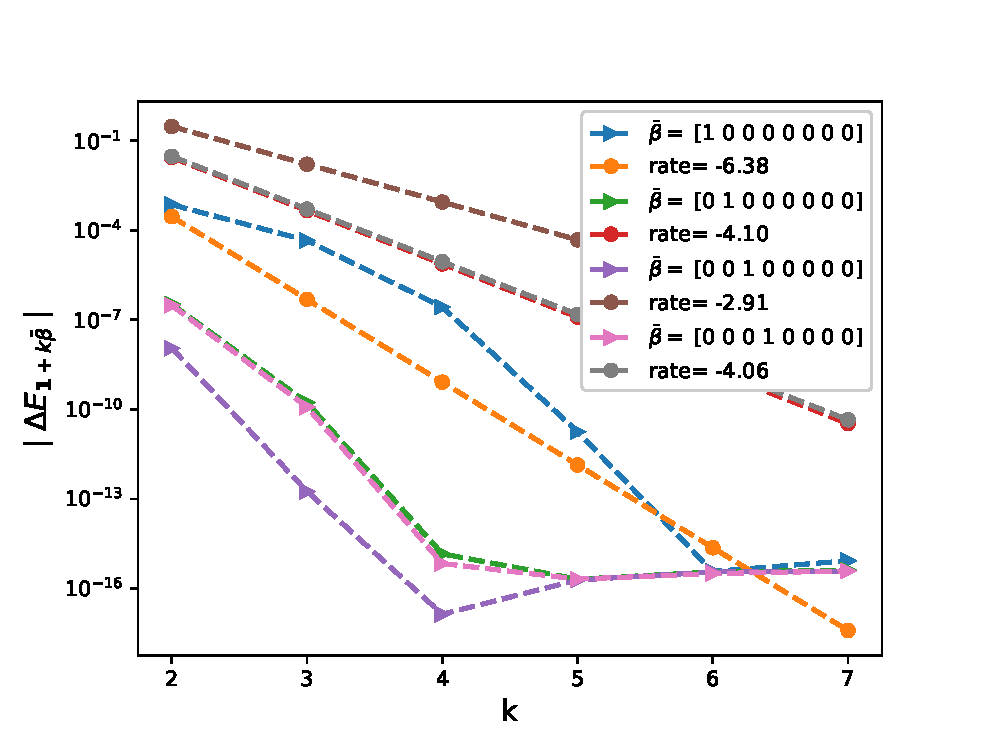
\includegraphics[width=1\linewidth]{./figures/rBergomi_mixed_error_rates/without_change_measure/N_4/H_002/first_difference_rbergomi_4steps_H_002_K_1_totally_hierarch_with_rate_W1}
		\caption{}
		\label{fig:sub3}
	\end{subfigure}%
	\begin{subfigure}{.4\textwidth}
		\centering
		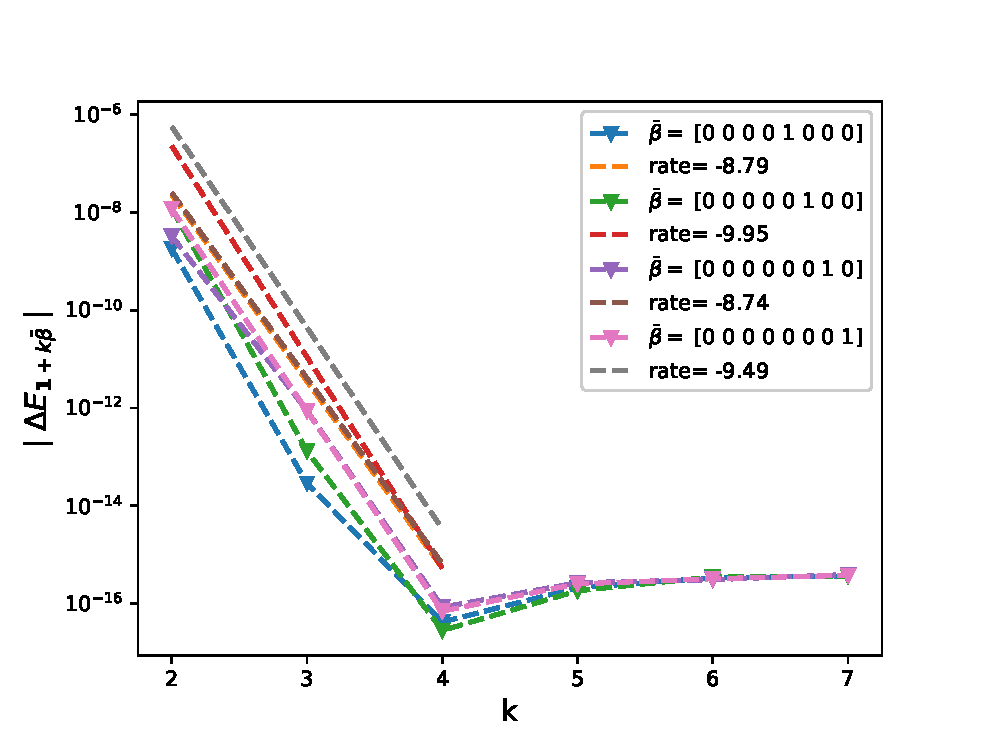
\includegraphics[width=1\linewidth]{./figures/rBergomi_mixed_error_rates/without_change_measure/N_4/H_002/first_difference_rbergomi_4steps_H_002_K_1_totally_hierarch_with_rate_W2}
		\caption{}
		\label{fig:sub4}
	\end{subfigure}
	
	
	
	\caption{The rate of error convergence of first order differences $\abs{\Delta \text{E}_{\boldsymbol{\beta}}}$ \eqref{eq:Work_error_contributions} ($\boldsymbol{\beta}=\mathbf{1}+k \bar{\boldsymbol{\beta}}$) with respect to $\mathbf{W}^{(1)}$ (a)  and  with respect to $\mathbf{W}^{(2)}$ (b), for parameter set $2$ in Table \ref{table:Reference solution, using MC with $500$ time steps, of Call option price under rBergomi model, for different parameter constellation.}. The number of quadrature points used in the $i$-th dimension is $N_i=2^{\beta_i-1}+1$. }
	\label{fig:first_diff_comp_K_1_H_002}
\end{figure}


\begin{figure}[h!]
	\centering
	\begin{subfigure}{.4\textwidth}
		\centering
		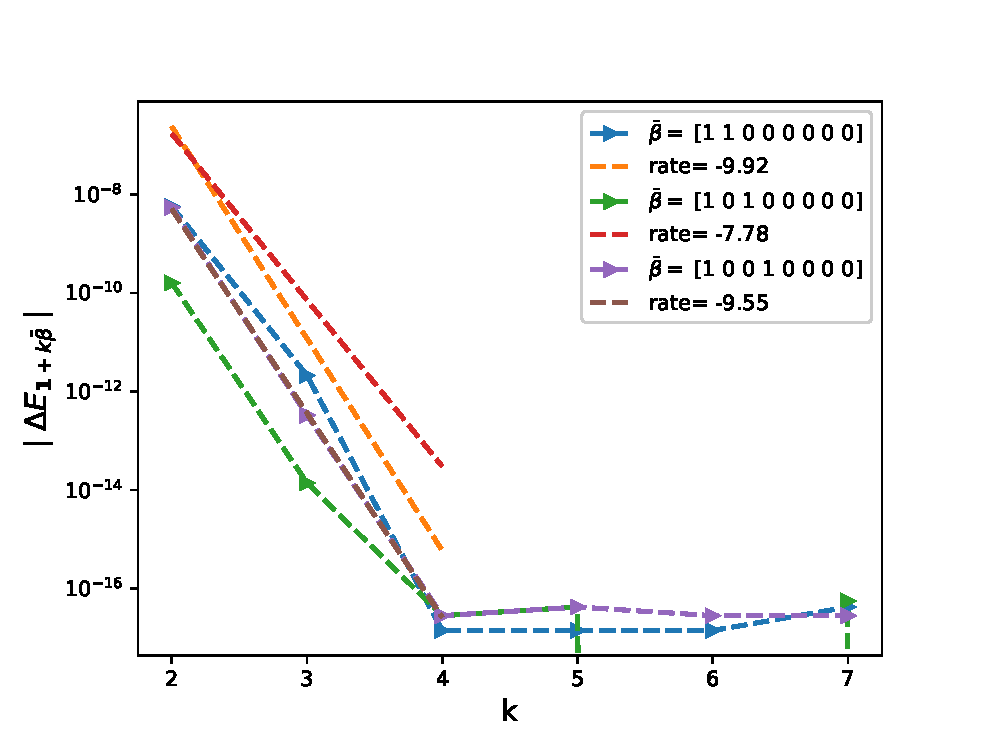
\includegraphics[width=1\linewidth]{./figures/rBergomi_mixed_error_rates/without_change_measure/N_4/H_002/mixed_difference_order2_rbergomi_4steps_H_002_K_1_totally_hierarch_with_rate_W1}
		\caption{}
		\label{fig:sub3}
	\end{subfigure}%
	\begin{subfigure}{.4\textwidth}
		\centering
		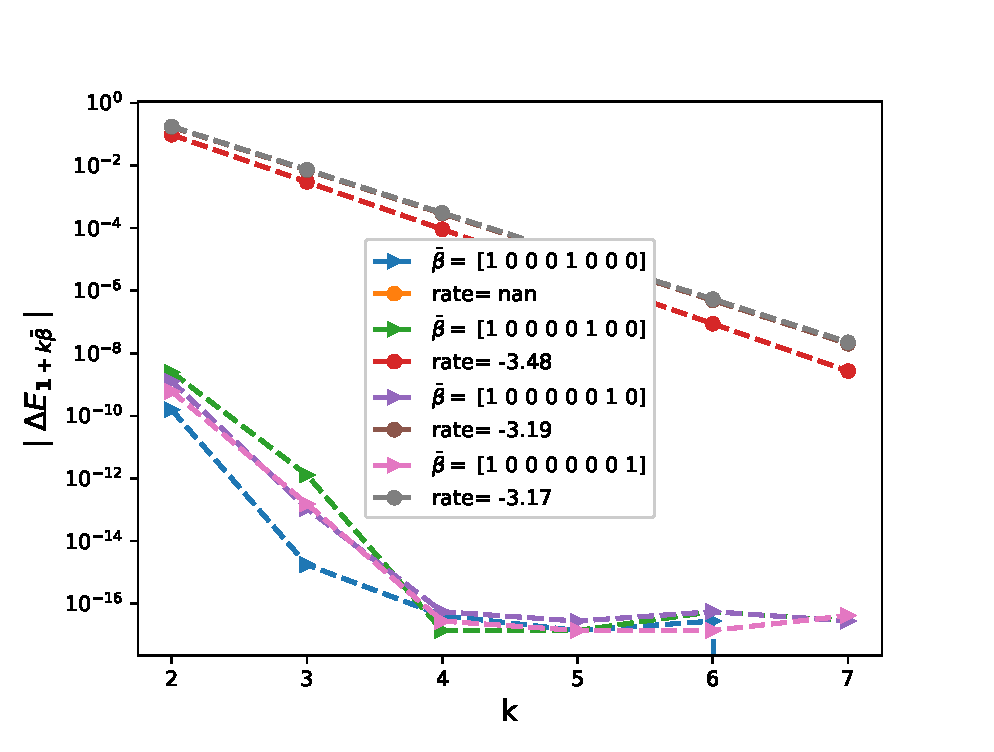
\includegraphics[width=1\linewidth]{./figures/rBergomi_mixed_error_rates/without_change_measure/N_4/H_002/mixed_difference_order2_rbergomi_4steps_H_002_K_1_totally_hierarch_with_rate_W2}
		\caption{}
		\label{fig:sub4}
	\end{subfigure}
	
	\caption{The rate of error convergence of  second order differences $\abs{\Delta \text{E}_{\boldsymbol{\beta}}}$ \eqref{eq:Work_error_contributions}  ($\boldsymbol{\beta}=\mathbf{1}+k \bar{\boldsymbol{\beta}}$) with respect to $\mathbf{W}^{(1)}$ (a)  and  with respect to $\mathbf{W}^{(2)}$ (b), for parameter set $2$ in Table \ref{table:Reference solution, using MC with $500$ time steps, of Call option price under rBergomi model, for different parameter constellation.}. The number of quadrature points used in the $i$-th dimension is $N_i=2^{\beta_i-1}+1$.}
	\label{fig:second_diff_comp_K_1_H_002}
\end{figure}

\FloatBarrier

%
%\begin{remark}
%	In this paper, we limited ourselves to designing a novel alternative method  based on hierarchical adaptive sparse grids quadrature for computing option prices under the rBergomi model. Giving the significant performance gains of our novel designed algorithm, we expect that designing a method based on QMC can bring similar or more gains as  our approach.
%\end{remark}



\subsection{Brownian bridge construction}\label{sec:Brwonian bridge construction}
In the literature of adaptive sparse grids and  QMC, several hierarchical path generation methods (PGMs) or transformation methods have been proposed to reduce the effective dimension. Among these transformations, we cite  the Brownian
bridge (Bb)  construction \cite{morokoff1994quasi,moskowitz1996smoothness,caflisch1997valuation}, the principal component analysis (PCA)  \cite{acworth1998comparison} and the linear transformation (LT) \cite{imai2004minimizing}.

In our context, the Brownian motion on a time discretization can be constructed either sequentially using a standard random walk construction or hierarchically using   other hierarchical PGMs as listed above. For our purposes, to make an effective use of MISC, which profits from anisotropy, we use the Bb construction since it produces  dimensions with different importance for MISC, contrary to random walk procedure for which all the dimensions of the stochastic space have equal importance.  This transformation  reduces the effective dimension  of the problem and as a consequence accelerates the MISC procedure by reducing the computational cost.


Let us denote $\{t_i\}_{i=0}^{N}$ the grid of time steps. Then the Bb construction \cite{glasserman2004monte} consists of the following: given a past value $B_{t_i}$ and a future value $B_{t_k}$, the value $B_{t_j}$ (with $t_i < t_j < t_k$) can be generated according to 
\begin{equation}
B_{t_j}=(1-\rho) B_{t_i}+\rho B_{t_k}+ \sqrt{\rho (1-\rho)(k-i) \Delta t} z, \: z \sim \mathcal{N}(0,1) \COMMA
\end{equation}
where $\rho=\frac{j-i}{k-i}$.  


%In particular, if $N$ is a power of $2$, then given $B_0=0$, Bb generates the Brownian motion at times $T, T/2,T/4,3T/4,\dots$ according
%\begin{align}\label{eq:BB construction}
%	B_T&=\sqrt{T}z_1\nonumber\\
%	B_{T/2}&= \frac{1}{2}(B_{0}+B_{T})+\sqrt{T/4}z_2= \frac{\sqrt{T}}{2} z_1+\frac{\sqrt{T}}{2} z_2\nonumber\\
%	B_{T/4}&=\frac{1}{2} (B_{0}+B_{T/2})+\sqrt{T/8}z_3= \frac{\sqrt{T}}{4} z_1+\frac{\sqrt{T}}{4} z_2+\sqrt{T/8}z_3\nonumber\\
%	\vdots \nonumber\\
%\end{align}
%where $\{z_j\}_{j=1}^{N}$ are independent standard normal variables.  In Bb construction scheme given by \eqref{eq:BB construction}, the most important values that determine the large scale structure of Brownian motion are the first components of $\mathbf{z} = (z_1,\dots,z_N)$.



%\begin{remark}
%In this paper, we chose to couple Brownian bridge construction with the MISC solver to reduce the effective dimension, since it is the less costly option in terms of computational work and the easiest to implement. We did not investigate the performance of MISC when coupling it with other hierarchical path generations method such as PCA or LT, which could be left as a future work that looks for the optimal PGM to couple with MISC in this context.
%\end{remark}
%


\subsection{Richardson extrapolation}\label{sec:Richardson extrapolation}


Another transformation that we coupled with MISC is Richardson extrapolation \cite{talay1990expansion}. In fact, applying level $K_\text{R}$ (level of extrapolation) of Richardson extrapolation reduces dramatically the bias and as a consequence reduces the  number of time steps $N$ needed in the coarsest level to achieve a certain error tolerance. This means basically that Richardson extrapolation directly reduces  the total dimension of the integration problem for achieving some error tolerance.


We  recall that the Euler scheme has weak order one so that

\begin{align}\label{Euler_weak_error}
	\abs{\expt{f(\hat{X}_T^h)}-\expt{f(X_T)} }  \leq C h
\end{align}

for some constant $C$, all sufficiently small $h$ and suitably smooth $f$. It can be easily  shown that  \eqref{Euler_weak_error} can be improved to


\begin{align}\label{Euler_weak_error_strenghten}
	\expt{f(\hat{X}_T^h)}= \expt{f(X_T)} + c h +\Ordo{h^2} \COMMA
\end{align}


where $c$ depends on $f$. 

Applying \eqref{Euler_weak_error_strenghten} with discretization step $2h$, we  obtain

\begin{align}\label{Euler_weak_error_strenghten_2h}
	\expt{f(\hat{X}_T^{2h})}= \expt{f(X_T)} + 2 c h +\Ordo{h^2} \COMMA
\end{align}

implying

\begin{align}\label{Richardson_extrapol}
	2 \expt{f(\hat{X}_T^{2h})}- \expt{f(\hat{X}_T^{h})} =\expt{f(X_T)} + \Ordo{h^2} \COMMA
\end{align}

For higher levels of extrapolations, we use the following: Let us denote by $h_J=h_0 2^{-J}$ the grid sizes (where $h_0$ is the coarsest grid size), by $K_\text{R}$ the level of the Richardson extrapolation, and by $I(J,K_\text{R})$ the approximation of $\expt{f((X_T)}$ by terms up to level $K_\text{R}$ (leading to a weak error of order $K_\text{R}$), then we have the following recursion 

\begin{align}
I(J,K_\text{R})=\frac{2^{K_\text{R}}\left[I(J,K_\text{R}-1)-I(J-1,K_\text{R}-1)\right]}{2^{K_\text{R}}-1},\quad J=1,2,\dots, K_\text{R}=1,2,\dots
\end{align}


\red{
\begin{remark}
We emphasize that through our work, we are interested in the pre-asymptotic regime (small number of time steps), and the use of Richardson extrapolation is justified by our observed experimental results in that regime (see Section \ref{sec:Weak error plots_no_change}),  which in, in particular, show an order one of convergence for the weak error. Although, we do not claim that the observed rates will scale well in the asymptotic regime, we observed that the pre-asymptotic regime is enough to get sufficiently accurate estimates for the option prices. 
\end{remark}
}





%\section{Details of Cholesky scheme coupled with hierarchical reresentation}\label{sec:Details of Cholesky scheme coupled with hierarchical reresentation}
%
%Let us denote by the matrix $A$, the computable covariance matrix of  $ \widetilde{W}^H_{t_1},\dots, \widetilde{W}_{t_N},W^1_{t_1},\dots, W^1_{t_N}$.  We can use Cholesky decomposition of $A$ to produce exact samples of $W^1_{t_1},\dots, W^1_{t_N}, \widetilde{W}^H_{t_1},\dots, \widetilde{W}_{t_N}$.

In fact let us denote by $L$ the triangular matrix resulting from Cholesky decomposition such that 
\[
L=
\left(
\begin{array}{c|c}
L_1& 0 \\
L_2 & L_3
\end{array}
\right),
\]
where $L_1, L_2,L_3$ are $N \times N$ matrices.

Then, given  a $2 N$-dimensional Gaussian random input vector, $\mathbf{X}=(X_1, \dots,X_N, X_{N+1}, \dots, X_{2N})$, we have

\begin{align}
\mathbf{W}^{(1)}=L_3 \mathbf{X}_{N+1:2N}, \quad \widetilde{\mathbf{W}}= 
\left(
\begin{array}{c}
L_1 \\
L_2 
\end{array}
\right) \mathbf{X}.
\end{align}
On the other hand, let us assume that we can construct $\mathbf{W}^{(1)}$ hierarchically  through  Brownian bridge construction defined by the linear mapping given by the matrix $G$, then given a $ N$-dimensional Gaussian random input vector, $\mathbf{Z}^\prime$, we can write
\begin{align*}
\mathbf{W}^{(1)}=G  \mathbf{Z}^\prime \COMMA
\end{align*}
and consequently
\begin{align*}
 \mathbf{X}_{N+1:2N}= L_3^{-1} G  \mathbf{Z}^\prime \PERIOD
\end{align*}
Therefore, given a $2 N$-dimensional Gaussian random input vector, $\mathbf{Z}=(\mathbf{Z}^\prime,\mathbf{Z}^{\prime \prime})$, we define our hierarchical representation by
\begin{align}\label{eq: Construction}
\mathbf{X}=\left(
\begin{array}{c|c}
0 & I_{N} \\
L_3^{-1} G & 0
\end{array}
\right) \mathbf{Z}.
\end{align}

We need to make sure that $\mathbf{X}$  have Gaussian distribution as an outcome of the construction \eqref{eq: Construction}. Consequently, we need to compute carefully $L_3^{-1}$.



\textbf{TO-DO $1$}: Implement the appropriate Cholesky scheme, taking into account the above construction, and check if the hierarchical construction is giving good results.




% \section{MISC error estimate}\label{sec:MISC error estimate}
%As discussed, potential ways of estimating the quadrature error are presented below.
\subsection{First way: Similar to the one implemented by Joakim}
I think this way is almost similar to the one implemented by Joakim. He may correct me if I missed some things.

In our case, once we fix $N$, we define from \eqref{BS_formula_rbergomi_2}
\begin{equation*}
F^N=C_{\text{BS}}(G(\mathbf{W}^{(1)},\mathbf{W}^{(2)})) \PERIOD
\end{equation*}
We introduce the set $C^0(\rset)$ of real-valued continuous functions over $\rset$, and the subspace of polynomials of degree at most $q$ over $\rset$, $\mathbb{P}^q(\rset) \subset C^0(\rset)$. Next,
we consider a sequence of univariate Lagrangian interpolant operators in each dimension $Y_n$ ($1 \le n \le 2N$), that is, $\{U_n^{m(\beta_n)}\}_{\beta_n \in \nset_+}$ (we refer to the value $\beta_n$ as the interpolation level). Each interpolant is built over a set of $m(\beta_n)$ collocation points, $\mathcal{H}^{m(\beta_n)}=\{y^1_n,y^2_n,\dots,y^{m(\beta_n)}_n\} \subset \rset$, thus, the interpolant yields a polynomial approximation,
\begin{equation*}
U^{m(\beta_n)}:C^0(\rset) \rightarrow \mathbb{P}^{m(\beta_n)-1}(\rset), \quad U^{m(\beta_n)}[F^N](y_n)= \sum_{j=1}^{m(\beta_n)} \left( f(y^j_n) \prod_{k=1;k \neq j}^{m(\beta_n)} \frac{y_n-y_n^k}{y_n^j-y_n^k}\right) \PERIOD
\end{equation*}
The $2N$-variate Lagrangian interpolant can then be built by a tensorization of univariate interpolants: denote by $C^0(\rset^{2N})$ the space of real-valued $2N$-variate continuous functions over $\rset^{2N}$ and by $\mathbb{P}^{\mathbf{q}}(\rset^{2N}) = \otimes_{n=1}^{2N} \mathbb{P}^{\mathbf{q}_n}(\rset)$ the subspace of polynomials of degree at most $q_n$ over $\rset$, with $\mathbf{q}=(q_1,\dots,q_{2N})\in  \nset^{2N}$, and consider a multi-index $\boldsymbol{\beta} \in \nset^{2N}_+$ assigning the interpolation level in each direction, $y_n$, then  the multivariate interpolant can then be written as
$$U^{m(\boldsymbol{\beta})}: C^0(\rset^{2N}) \rightarrow \mathbb{P}^{m(\boldsymbol{\beta})-1}(\rset^{2N}) ,\quad  U^{m(\boldsymbol{\beta})}[F^N](\mathbf{y})= \bigotimes_{n = 1}^{2N} U^{m(\beta_n)} [F^N](\mathbf{y}) \PERIOD $$
Given this construction, we can define the ASGQ interpolant  for approximating $F^N$, using a set of multi indices $\mathcal{I} \in \nset^{2N}$ as
\begin{equation}
I^{\mathcal{I}}[F^N]= \sum_{\boldsymbol{\beta} \in \mathcal{I}} \Delta U_N^{\boldsymbol{\beta}} \COMMA
\end{equation}
where 
\begin{equation*}
\Delta_i U_N^{\boldsymbol{\beta}} = \left\{ 
\aligned 
 U_N^{\boldsymbol{\beta}} &- U_N^{\boldsymbol{\beta}'}  \text{, with } \boldsymbol{\beta}' =\boldsymbol{\beta} - e_i, \text{ if } \boldsymbol{\beta}_i>0 \\
 U_N^{\boldsymbol{\beta}} &, \quad  \text{ otherwise,}
\endaligned
\right.
\end{equation*}
where $e_i$ denotes the $i$th $2N$-dimensional unit vector. Then, $\Delta
U_N^{\boldsymbol{\beta}}$ is defined as
\begin{equation*}
\Delta U_N^{\boldsymbol{\beta}} = \left( \prod_{i=1}^{2N} \Delta_i \right) U_N^{\boldsymbol{\beta}}.
\end{equation*}
We define the interpolation error induced by ASGQ as
\begin{equation}
e_{N}= F^N-I^{\mathcal{I}}[F^N] \PERIOD
\end{equation}
One can have a bound on the interpolation error of ASGQ, $e_{N}$, by tensorizing one dimensional error estimates, and  then simply integrate that bound to get the ASGQ  error, $\mathcal{E}_Q(\text{TOL}_{\text{ASGQ}},N)$, defined in \eqref{eq:total_error_ASGQ}. However, we think that this will  not lead to a sharp error estimate for ASGQ. Another strategy for estimating the ASGQ  error, is to estimate $\expt{e_N}$ using MC by sampling directly $e_N$ (what I think Jaokim code is doing actually) .

If we define $Y=F^N+(Q_N^{\mathcal{I}}-I^{\mathcal{I}}[F^N])$ (where $Q_N^{\mathcal{I}}$ is the ASGQ  estimator), then we have
\begin{align}\label{eq:Control_variate}
\expt{Y}&=\expt{F^N}\nonumber\\
Var[Y]&=Var[e_N]< Var[\mathcal{A}_{\text{MC}}]\COMMA
\end{align}
where $\mathcal{A}_{\text{MC}}$ is the MC estimator for $\expt{F^N}$.

\eqref{eq:Control_variate} shows that ASGQ can be seen as a control variate for MC estimator and consequently as a powerful variance reduction tool.

This way of estimating the quadrature error comes with the disadvantage of exciting the strong error which has a poor behavior in our context resulting maybe to having a non-sharp error estimate. In fact, by the central limit theorem, we expect that
\begin{align}\label{eq:CLT_interpol_errror}
\abs{\expt{e_N}}&=\abs{\int \underbrace{F^N-I^{\mathcal{I}}[F^N](y)}_{Y(y)} dy}\nonumber\\
&\approx \frac{C_\alpha}{\sqrt{M}} \sqrt{\text{Var(Y)}}\PERIOD
\end{align}
In our context of the rBergomi model we know that the strong error is of order $H$, that is we expect to have $\text{Var(Y)}=\Ordo{h^H}$ ($h$ is the mesh size and $H$ is the Hurst parameter which is of order $\approx 0.1$. As a consequence, it may be that using this way will not provide a sharp enough error estimate for the quadrature error!

\subsection{Second way}
To avoid exciting the strong error when estimating the quadrature error and just act on the weak error, we can use a second way that is inspired of randomized QMC. In fact, we suggest to use a randomized version of ASGQ where the randomization involves randomized rotation and scaling for quadrature rules since we deal with unbounded domains and Hermite quadrature rule. Although this comes with the advantage of just acting on the weak error, it has the issue of reducing anisotropy which is a main feature for a good performance of ASGQ.

We can formulate this more in case the first way fail!

\subsection{Third way}
One can learn the error curve as a way to reduce the extra burden that comes
from estimating the ASGQ error but this not yet formulated yet. I will try to formulate it if the two previous options fail!

  \section{Numerical experiments}\label{sec:Numerical tests}


\subsection{Summary of the numerical results}

We conduct our experiments for $5$ different parameters  sets as presented in tables \ref{table:Reference solution, using MC with $500$ time steps, of Call option price under rBergomi model, for different parameter constellation.}. 

In Section \ref{sec:Weak error plots_no_change}, we estimate the weak error  (Bias) for the different parameter constellations, for $2$ scenarios involving with/without  Richardson extrapolation. The conclusions of this section are: 
\begin{itemize}
	\item Without Richardson extrapolation: For all cases except parameters set $4$, we get a weak error of order $\Delta t$, with different  constants. Interestingly, we see that the case of parameters set $4$ (see table \ref{table:Reference solution, using MC with $500$ time steps, of Call option price under rBergomi model, for different parameter constellation.}) has a weak error rate of order around $0.4$ but with a small constant. 
	
		\item With Richardson extrapolation: For all reported cases (sets  $1,2,3$ in table \ref{table:Reference solution, using MC with $500$ time steps, of Call option price under rBergomi model, for different parameter constellation.}), we get an improvement for weak error in terms of the rate and constants compared to the case without Richardson extrapolation.
\end{itemize}

\begin{remark}
We emphasize that the reported weak rates correspond to the pre-asymptotic regime that we are interested in. We are not interested on estimating the rates specifically but rather a sufficient precise estimate of the weak error (Bias), $\mathcal{E}_B(N)$, for different time steps $N$, in order to get the biased MC  solution for a given discretization, that we denoted $Q^N(\infty)$ in Section \ref{sec:Details of the MISC}.  For a fixed discretization, the corresponding biased solution will be set as a reference solution to the MISC solver in order to estimate the quadrature error $\mathcal{E}_Q(TOL_{\text{MISC}},N)$.	
\end{remark}

In Section \ref{sec:Comparing different  errors and complexity for MC and MISC}, we show tables and plots reporting  the different errors involved in MC method (bias and statistical error), related to the plots in Section \ref{sec:Weak error plots_no_change}, and in MISC (Quadrature error). We do this for each case of parameter set. The quadrature error (see \eqref{eq:quadrature error}) is computed by subtracting the MISC solution from the biased solution, computed with sufficiently large  number of samples (to kill the statistical error). Given that both methods, MC and MISC, have the same bias,  the computational time of MC and MISC is compared such that the statistical error is almost equal to the stable quadrature error produced by MISC.

 The conclusions of this section are: 


	\begin{enumerate}
		
		
		\item [i)] For the case of set $1$ (See Section \ref{sec:Case of set 1 parameters}), MISC coupled with Richardson extrapolation  is $3$ times faster than MC coupled with Richardson extrapolation, to achieve a total relative error around $8\%$  (see  tables(\ref{Total  error of MISC and MC to compute Call option price of the different tolerances for different number of time steps. Case set $1$ parameters, with Richardson extrapolation(level $1$). The numbers between parentheses are the corresponding absolute errors.}, \ref{Comparsion of the computational time of  MC and MISC, using Richardson extrapolation (level $1$), used to compute Call option price of rBergomi model for different number of time steps. Case set $1$ parameters})). This gain is improved when applying level $2$ Richardson extrapolation. In fact,  MISC coupled with Richardson extrapolation (level $2$) is $4$ times faster than MC coupled with Richardson extrapolation (level $2$), to achieve a total relative error around $0.5\%$ (see  tables  ( \ref{Total  error of MISC and MC to compute Call option price of the different tolerances for different number of time steps. Case set $1$ parameters, with Richardson extrapolation(level $2$). The numbers between parentheses are the corresponding absolute errors.}, \ref{Comparsion of the computational time of  MC and MISC, using Richardson extrapolation (level $2$), used to compute Call option price of rBergomi model for different number of time steps. Case set $1$ parameters})).  Applying Richardson extrapolation brought a significant improvement for MISC (compare tables (\ref{Total error of MISC and MC to compute Call option price of the different tolerances for different number of time steps. Case set 1, without Richardson extrapolation. The numbers between parentheses are the corresponding absolute errors.},\ref{Comparison of the computational time of  MC and MISC, used to compute Call option price of rBergomi model for different number of time steps. Case set1}) (no Richardson), tables (\ref{Total  error of MISC and MC to compute Call option price of the different tolerances for different number of time steps. Case set $1$ parameters, with Richardson extrapolation(level $1$). The numbers between parentheses are the corresponding absolute errors.}, \ref{Comparsion of the computational time of  MC and MISC, using Richardson extrapolation (level $1$), used to compute Call option price of rBergomi model for different number of time steps. Case set $1$ parameters}) (Richardson (level $1$)) and  tables ((\ref{Total  error of MISC and MC to compute Call option price of the different tolerances for different number of time steps. Case set $1$ parameters, with Richardson extrapolation(level $2$). The numbers between parentheses are the corresponding absolute errors.}, \ref{Comparsion of the computational time of  MC and MISC, using Richardson extrapolation (level $2$), used to compute Call option price of rBergomi model for different number of time steps. Case set $1$ parameters})) (Richardson (level $2$)), also see  figure \ref{fig:Complexity plot for  MISC for Case set $1$ parameters, comparison}).
		
			\item [ii)] For the case of set $2$ (See Section \ref{sec:Case of set $2$ parameters_linear}), MISC coupled with Richardson extrapolation is $19$ times faster than MC coupled with Richardson extrapolation, to achieve a total relative error around $8\%$ and $4$ times faster than MC, to achieve total relative error around $2\%$ (see tables (\ref{Total  error of MISC and MC to compute Call option price of the different tolerances for different number of time steps. Case set $2$ parameters, with Richardson extrapolation(level $1$). The numbers between parentheses are the corresponding absolute errors,relative},\ref{Comparsion of the computational time of  MC and MISC, using Richardson extrapolation (level $1$), used to compute Call option price of rBergomi model for different number of time steps. Case set $2$ parameters,linear})). This gain is improved when applying level $2$ Richardson extrapolation. In fact,  MISC coupled with Richardson extrapolation (level $2$) is $17$ times faster than MC coupled with Richardson extrapolation (level $2$), to achieve a total relative error below  $1\%$ (see  tables (\ref{Total  error of MISC and MC to compute Call option price of the different tolerances for different number of time steps. Case set $2$ parameters, with Richardson extrapolation(level $2$). The numbers between parentheses are the corresponding absolute errors,linear}, \ref{Comparsion of the computational time of  MC and MISC, using Richardson extrapolation (level $2$), used to compute Call option price of rBergomi model for different number of time steps. Case set $2$ parameters,linear})). Applying Richardson extrapolation brought a significant improvement for MISC (compare tables (\ref{Total error of MISC and MC to compute Call option price of the different tolerances for different number of time steps. Case $K=1$, $H=0.07$, without Richardson extrapolation. The numbers between parentheses are the corresponding absolute errors,linear}, \ref{Comparsion of the computational time of  MC and MISC, used to compute Call option price of rBergomi model for different number of time steps. Case $K=1, H=0.07$, linear}) (no Richardson), tables (\ref{Total  error of MISC and MC to compute Call option price of the different tolerances for different number of time steps. Case set $2$ parameters, with Richardson extrapolation(level $1$). The numbers between parentheses are the corresponding absolute errors,relative},\ref{Comparsion of the computational time of  MC and MISC, using Richardson extrapolation (level $1$), used to compute Call option price of rBergomi model for different number of time steps. Case set $2$ parameters,linear}) (Richardson (level $1$)) and  tables  (\ref{Total  error of MISC and MC to compute Call option price of the different tolerances for different number of time steps. Case set $2$ parameters, with Richardson extrapolation(level $2$). The numbers between parentheses are the corresponding absolute errors,linear}, \ref{Comparsion of the computational time of  MC and MISC, using Richardson extrapolation (level $2$), used to compute Call option price of rBergomi model for different number of time steps. Case set $2$ parameters,linear}) (Richardson (level $2$))).
		
		
		
		
			\item [iii)]  For the case of set $3$ (See Section \ref{sec:Case of set 3 parameters}), MISC is  $35$ times faster than MC, to achieve  a total relative error below $1\%$ and $8$ times faster than MC, to achieve a total relative error around $0.1\%$ (see figure \ref{fig:Complexity plot for MC and MISC for Case set $3$ parameters} and tables (\ref{Comparsion of the computational time of  MC and MISC, used to compute Call option price of rBergomi model for different number of time steps. Case set3}, \ref{Total error of MISC and MC to compute Call option price of the different tolerances for different number of time steps. Case set 3, without Richardson extrapolation. The numbers between parentheses are the corresponding absolute errors.})). Using Richardson extrapolation brought an improvement in terms of the  complexity constant compared to using simple MISC (See figure \ref{fig:Complexity plot for  MISC for case set $3$ parameters, comparison} and tables (\ref{Total  error of MISC and MC to compute Call option price of the different tolerances for different number of time steps. Case set $3$ parameters, with Richardson extrapolation(level $1$). The numbers between parentheses are the corresponding absolute errors.}, \ref{Comparsion of the computational time of  MC and MISC, using Richardson extrapolation (level $1$), used to compute Call option price of rBergomi model for different number of time steps. Case set $3$ parameters})).
				
	 	\item [iv)] For the case of set $4$ (See Section \ref{sec:Case of set 4 parameters}), MISC is  $141$ times faster than MC, to achieve a total relative error below $1\%$ (see figure \ref{fig:Complexity plot for MC and MISC for case set $4$ parameters} and tables (\ref{Comparsion of the computational time of  MC and MISC, used to compute Call option price of rBergomi model for different number of time steps. Case set4}, \ref{Total error of MISC and MC to compute Call option price of the different tolerances for different number of time steps. Case set 4, without Richardson extrapolation. The numbers between parentheses are the corresponding absolute errors.})).
		
	\item [v)] For the case of set $5$ (See Section \ref{sec:Case of set 5 parameters}), MISC is  $220$ times faster than MC, to achieve a total relative error below $6\%$ and $16$ times faster than MC, to achieve total relative error around $2\%$  (see figure \ref{fig:Complexity plot for MC and MISC for Case set $5$ parameters} and tables (\ref{Comparsion of the computational time of  MC and MISC, used to compute Call option price of rBergomi model for different number of time steps. Case set5}, \ref{Total error of MISC and MC to compute Call option price of the different tolerances for different number of time steps. Case set 5, without Richardson extrapolation. The numbers between parentheses are the corresponding absolute errors.})).
		
	\end{enumerate}

	
	











\subsection{Weak error plots} \label{sec:Weak error plots_no_change}
In this section, we include the results of weak errors for the different parameters sets as in table \ref{table:Reference solution, using MC with $500$ time steps, of Call option price under rBergomi model, for different parameter constellation.}, with and without Richardson extrapolation.  We considered a number of time steps $N \in \{2,4,8,16\}$.  The options are priced in terms of the moneyness $K$, where $K$ is the strike price.  The reference solution was computed with $N=500$ time steps (reported in table \ref{table:Reference solution, using MC with $500$ time steps, of Call option price under rBergomi model, for different parameter constellation.}). We note that the weak errors plotted here correspond to relative errors. We show in table \ref{table:Reference solution, using MC with $500$ time steps, of Call option price under rBergomi model, for different parameter constellation.} the different parameter constellations that we consider to report our results for MC and MISC.



\begin{table}[!h]
	\centering
	\begin{tabular}{l*{2}{c}r}
		Parameters            & Reference solution    \\
	Set $1$:	$H=0.43, K=1,S_0=1, \rho=-0.9, \eta=1.9,\xi=0.235^2$   & $\underset{(5.7e-05)}{0.0712074}$  \\	
			Set $2$:	$H=0.07, K=1,S_0=1, \rho=-0.9, \eta=1.9,\xi=0.235^2$   & $\underset{(7.9e-05)}{0.0790852}$  \\	

				Set $3$:	$H=0.02, K=1,,S_0=1, \rho=-0.7, \eta=0.4,\xi=0.1$   & $\underset{(1.3e-04)}{0.1247563}$  \\
					Set $4$:	$H=0.02, K=0.8,S_0=1, \rho=-0.7, \eta=0.4,\xi=0.1$   & $\underset{(5.6e-04)}{0.2407117}$  \\
						Set $5$:	$H=0.02, K=1.2,S_0=1, \rho=-0.7, \eta=0.4,\xi=0.1$   & $\underset{(2.5e-04)}{0.0568394}$  \\
		\hline
	\end{tabular}
	\caption{Reference solution, using MC with $500$ time steps and $M=10^6$, of call option price under rBergomi model, for different parameter constellation.  The numbers between parentheses correspond to the statistical errors.}
	\label{table:Reference solution, using MC with $500$ time steps, of Call option price under rBergomi model, for different parameter constellation.}
\end{table}
\FloatBarrier


\subsubsection{Without Richardson extrapolation}
From figures (\ref{fig:Weak_rate_set1_set_2_without_rich},\ref{fig:Weak_rate_H_002_without_rich_K_1_K_08},\ref{fig:Weak_rate_H_002_without_rich_K_12}), we see that for all cases  except parameters set $4$, we get a weak error of order $\Delta t$, with different  constants. Interestingly, we see that the case of parameters set $4$ (see table \ref{table:Reference solution, using MC with $500$ time steps, of Call option price under rBergomi model, for different parameter constellation.}) has a weak error rate of order around $0.4$ but with a small constant. The upper and lower bounds are $95\%$ confidence intervals.


\begin{figure}[h!]
	\centering
	\begin{subfigure}{.4\textwidth}
		\centering
		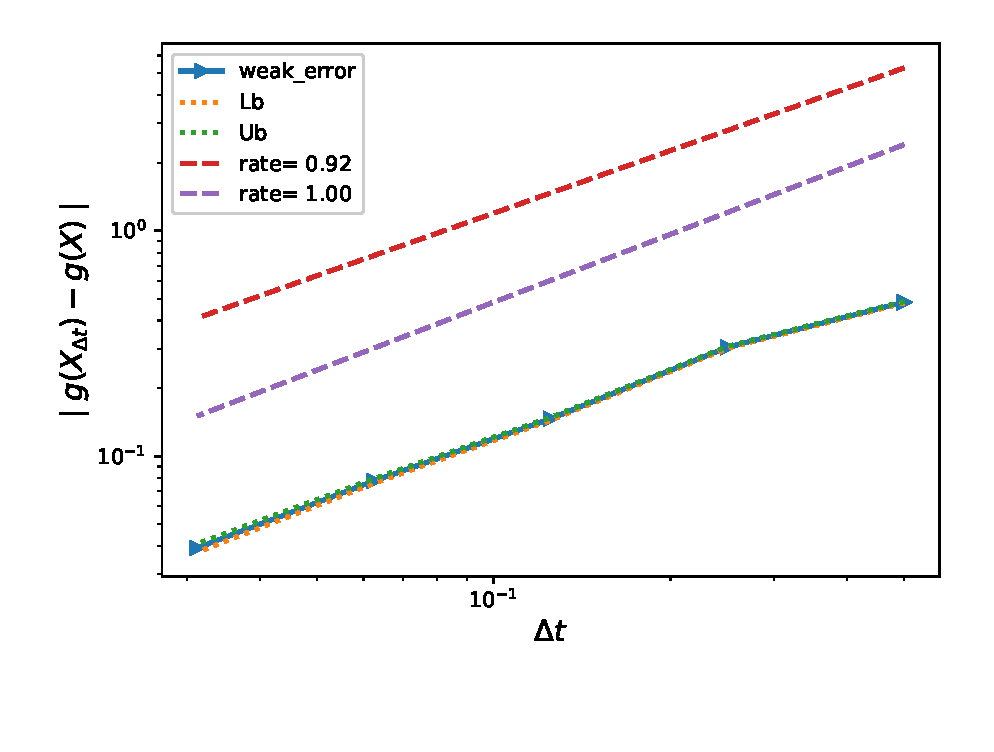
\includegraphics[width=1\linewidth]{./figures/rBergomi_weak_error_rates/without_richardson/H_043/weak_convergence_order_Bergomi_H_043_K_1_M_10_6_CI_relative}
		\caption{}
		\label{fig:sub3}
	\end{subfigure}%
	\begin{subfigure}{.4\textwidth}
		\centering
		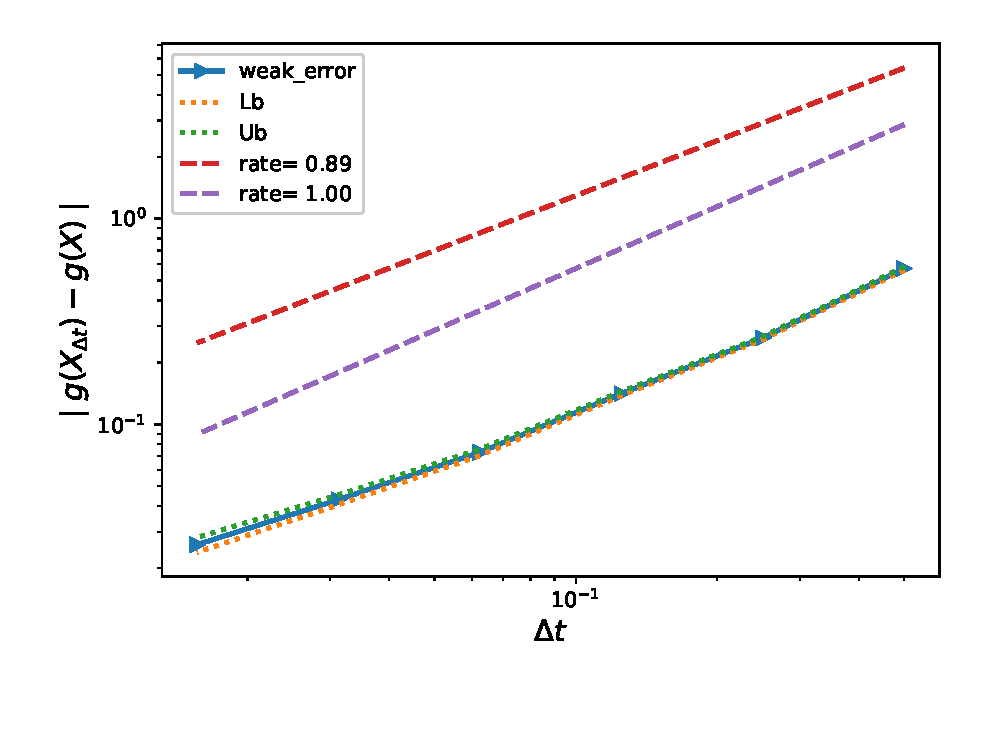
\includegraphics[width=1\linewidth]{./figures/rBergomi_weak_error_rates/without_richardson/H_007/weak_convergence_order_Bergomi_H_007_K_1_M_10_6_CI_relative}
		\caption{}
		\label{fig:sub4}
	\end{subfigure}
	
	\caption{The rate of convergence of the weak error  $\abs{\expt{g(X_{\Delta t})}-g(X)}$  without Richardson extraploation, using MC with $M=10^6$: a) Set $1$ parameters in table \ref{table:Reference solution, using MC with $500$ time steps, of Call option price under rBergomi model, for different parameter constellation.}.  b) Set $2$ parameters in table \ref{table:Reference solution, using MC with $500$ time steps, of Call option price under rBergomi model, for different parameter constellation.}.}
	\label{fig:Weak_rate_set1_set_2_without_rich}
\end{figure}





\begin{figure}[!htb]
	\centering
	\begin{subfigure}{.4\textwidth}
		\centering
		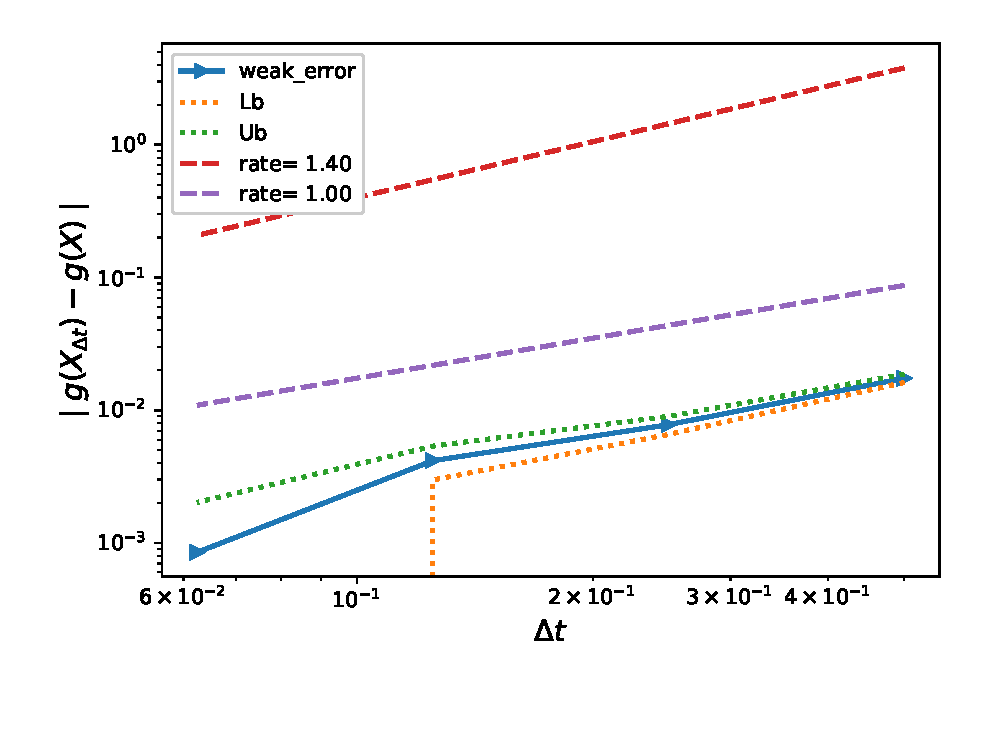
\includegraphics[width=1\linewidth]{./figures/rBergomi_weak_error_rates/without_richardson/H_002/weak_convergence_order_Bergomi_H_002_K_1_M_3_10_6_CI_relative}
		\caption{}
		\label{fig:sub3}
	\end{subfigure}%
	\begin{subfigure}{.4\textwidth}
		\centering
		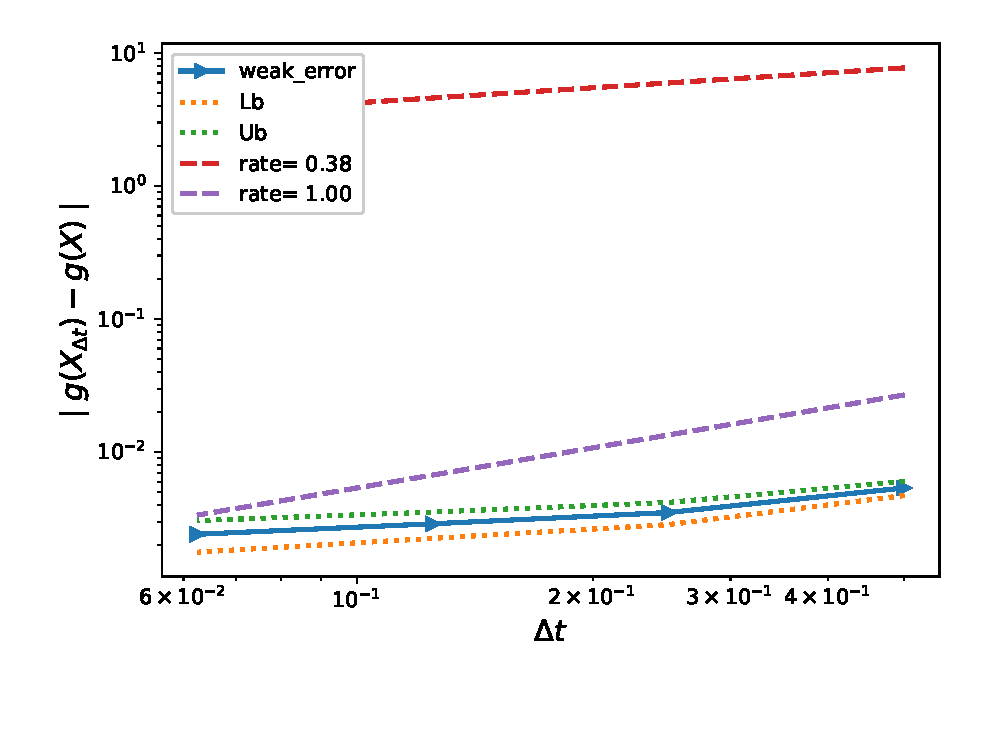
\includegraphics[width=1\linewidth]{./figures/rBergomi_weak_error_rates/without_richardson/H_002/weak_convergence_order_Bergomi_H_002_K_08_M_5_10_6_CI_relative}
		\caption{}
		\label{fig:sub4}
	\end{subfigure}
	
	\caption{The rate of convergence of the weak error $\abs{\expt{g(X_{\Delta t})}-g(X)}$  without Richardson extraploation, using MC with $M=5.10^6$: a) Set $3$ parameters in table \ref{table:Reference solution, using MC with $500$ time steps, of Call option price under rBergomi model, for different parameter constellation.},  b) Set $4$ parameters in table \ref{table:Reference solution, using MC with $500$ time steps, of Call option price under rBergomi model, for different parameter constellation.}. }
	\label{fig:Weak_rate_H_002_without_rich_K_1_K_08}
\end{figure}











\begin{figure}[!htb]
		\centering
		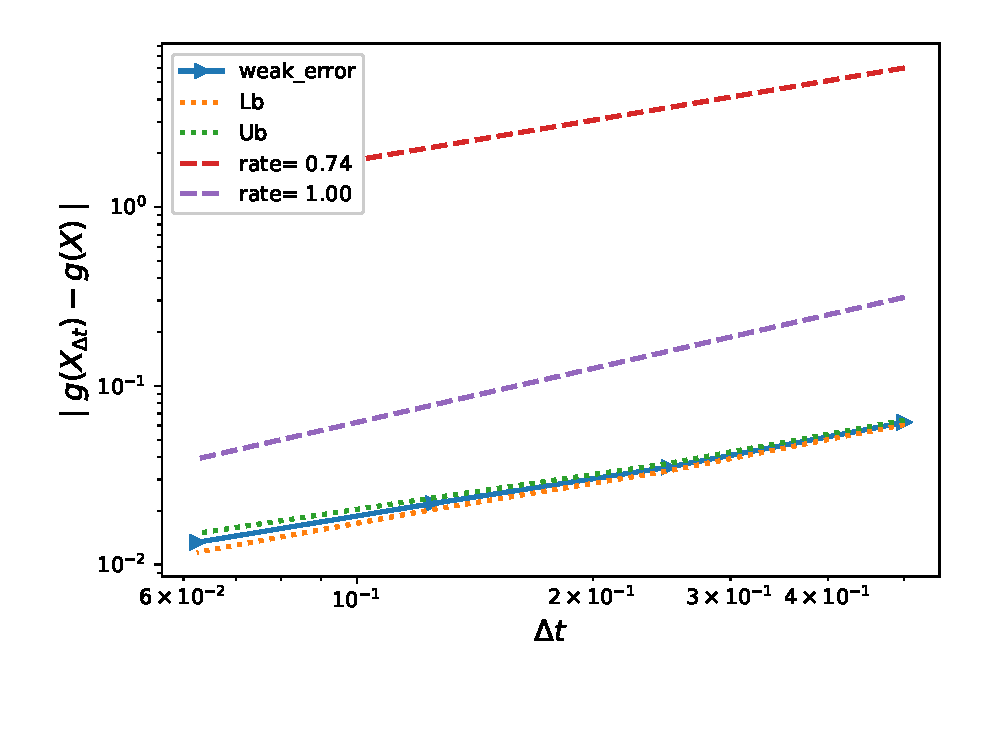
\includegraphics[width=0.4\linewidth]{./figures/rBergomi_weak_error_rates/without_richardson/H_002/weak_convergence_order_Bergomi_H_002_K_12_M_3_10_6_CI_relative}	
	\caption{The rate of convergence of the weak error $\abs{\expt{g(X_{\Delta t})}-g(X)}$, for set $5$ parameters in table \ref{table:Reference solution, using MC with $500$ time steps, of Call option price under rBergomi model, for different parameter constellation.}, without Richardson extraploation, using MC with $M=5.10^6$.}
	\label{fig:Weak_rate_H_002_without_rich_K_12}
\end{figure}


\FloatBarrier


\subsubsection{With Richardson extrapolation (level 1)}
Figures (\ref{fig:Weak_rate_H_043_007_with_rich}, \ref{fig:Weak_rate_H_002_with_rich_K1}) illustrate the weak errors estimates for parameters sets $1,2,3$ in table \ref{table:Reference solution, using MC with $500$ time steps, of Call option price under rBergomi model, for different parameter constellation.}. The upper and lower bounds are $95\%$ confidence intervals.
\begin{figure}[h!]
	\centering
	\begin{subfigure}{.4\textwidth}
		\centering
		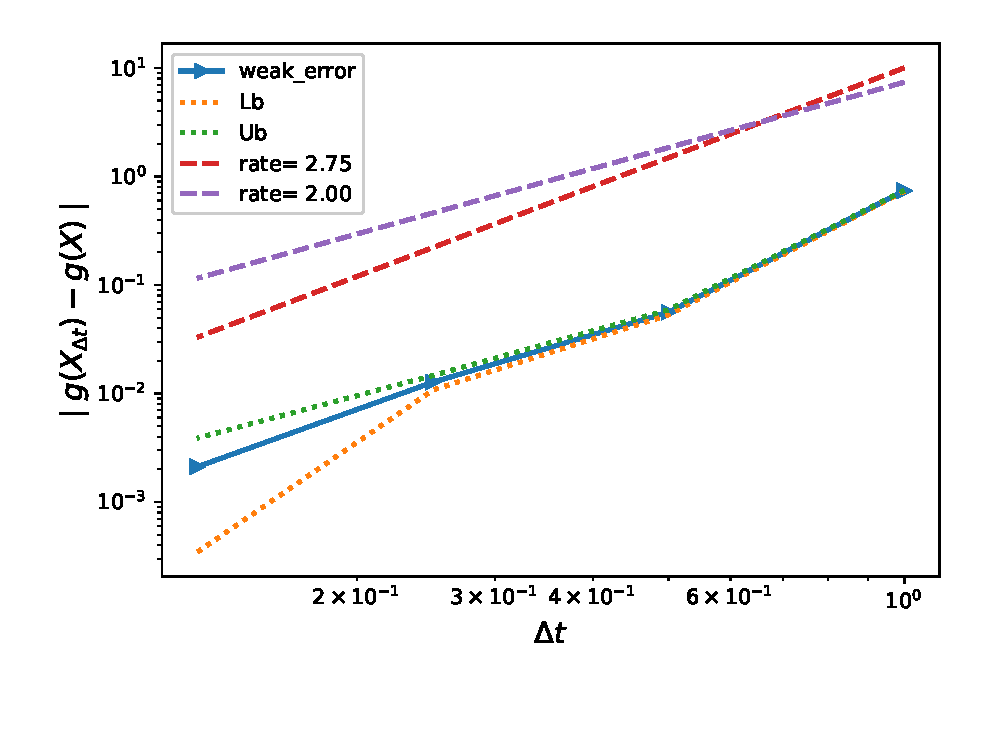
\includegraphics[width=1\linewidth]{./figures/rBergomi_weak_error_rates/with_richardson/H_043/weak_convergence_order_Bergomi_H_043_K_1_M_10_6_richardson_relative}
		\caption{}
		\label{fig:sub3}
	\end{subfigure}%
	\begin{subfigure}{.4\textwidth}
		\centering
		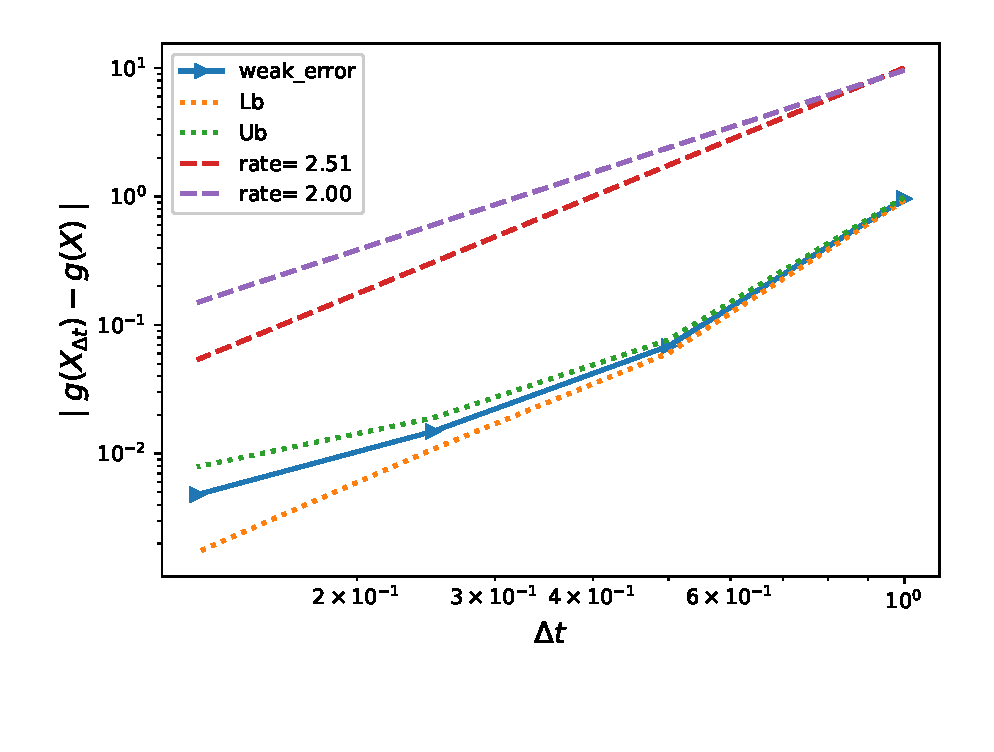
\includegraphics[width=1\linewidth]{./figures/rBergomi_weak_error_rates/with_richardson/H_007/weak_convergence_order_Bergomi_H_007_K_1_richardson_relative_M_10_6}
		\caption{}
		\label{fig:sub4}
	\end{subfigure}
	
	\caption{The rate of convergence of the weak error  $\abs{\expt{2 g(X_{\Delta t/2}) -g(X_{\Delta t})}-g(X)}$   with Richardson extraploation, using MC with $M=10^6$: a) Set $1$ parameters in table \ref{table:Reference solution, using MC with $500$ time steps, of Call option price under rBergomi model, for different parameter constellation.}.  b) Set $2$ parameters in table \ref{table:Reference solution, using MC with $500$ time steps, of Call option price under rBergomi model, for different parameter constellation.}, }
	\label{fig:Weak_rate_H_043_007_with_rich}
\end{figure}




\begin{figure}[!htbp]
	\centering
		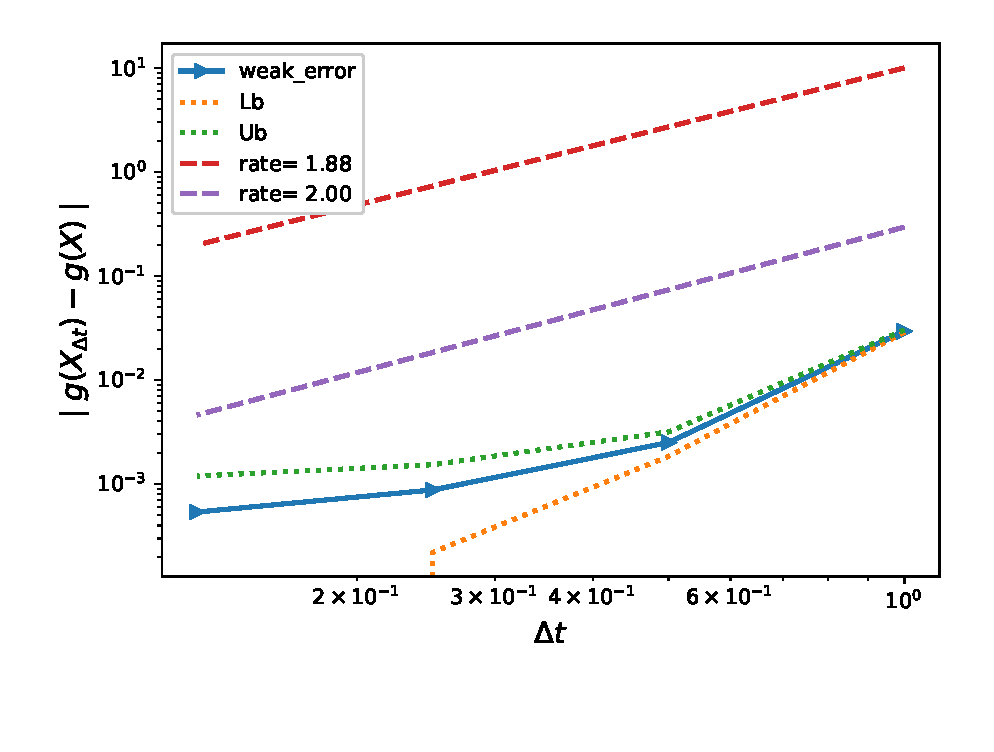
\includegraphics[width=0.4\linewidth]{./figures/rBergomi_weak_error_rates/with_richardson/H_002/weak_convergence_order_Bergomi_H_002_K_1_M_1_10_7_richardson_relative}
	\caption{The rate of convergence of the weak error $\abs{\expt{2 g(X_{\Delta t/2}) -g(X_{\Delta t})}-g(X)}$,  for set $3$ parameters in table \ref{table:Reference solution, using MC with $500$ time steps, of Call option price under rBergomi model, for different parameter constellation.}, with Richardson extraploation, using MC with $M=10^7$. }
	\label{fig:Weak_rate_H_002_with_rich_K1}
\end{figure}
\FloatBarrier




\subsection{Comparing different  errors and complexity for MC and MISC}\label{sec:Comparing different  errors and complexity for MC and MISC}


The results were reported for the different sets of parameters defined in table \ref{table:Reference solution, using MC with $500$ time steps, of Call option price under rBergomi model, for different parameter constellation.}. We considered   a number of time steps $N \in \{2,4,8,16\}$.  The options are priced in terms of the moneyness $K$, where $K$ is the strike price.   

 For each set,  we report the results for $2$ scenarios: i) Without using Richardson extrapolation and  ii) Using level $1$ Richardson extrapoaltion.

In each case, we show a table of computed values using MISC with different tolerances as well the biased MC value, using large number of samples to kill the statistical error. Then, in a second table,  we show the bias as well the statistical error for MC method, related to Section \ref{sec:Weak error plots_no_change}. After that, a plot  shows the behavior of  the relative quadrature error which is computed as the normalized difference between the biased MC solution and MISC solution. Then, we provide the total relative error which is the sum of the bias and statistical error for MC, and the quadrature error for MISC. We note that we used a number of samples for MC such that the statistical error is almost equal to the stable quadrature error, in order to have a fair complexity comparison between the two methods. Finally, we show the CPU time needed for each solver. We note that  in all cases the actual work (runtime) was obtained using a $40$-core Intel(R) Xeon(R) CPU E5-268 architecture.

\subsubsection{Case of set $1$ parameters in table \ref{table:Reference solution, using MC with $500$ time steps, of Call option price under rBergomi model, for different parameter constellation.}}\label{sec:Case of set 1 parameters}

\subsubsection*{Without Richardson extrapolation}
\begin{table}[h!]
	\centering
	\begin{tabular}{l*{6}{c}r}
		Method \textbackslash  Steps            & $2$ & $4$ & $8$ & $16$ &   \\
		\hline
%		MISC ($TOL_{\text{MISC}}=5.10^{-1}$)  & $0.1140$ & $0.0961$ & $0.0848$ & $0.0781$  \\
		MISC ($TOL_{\text{MISC}}=10^{-1}$)  & $0.1140$ & $0.0961$ & $0.0871$ & $0.0802$  \\
%		MISC ($TOL_{\text{MISC}}=5.10^{-2}$)  & $0.1140$ & $0.0963$ & $0.0843$ & $0.0824$  \\
		MISC ($TOL_{\text{MISC}}=10^{-2}$)  & $0.1077$ & $0.0944$ & $0.0838$ & $0.0772$  \\

		MISC ($TOL_{\text{MISC}}=10^{-3}$)  & $0.1077$ & $0.0921$ & $0.0819$ & $0.0762$  \\
%		MISC ($TOL_{\text{MISC}}=5.10^{-4}$)  & $0.1079   $ & $0.0921$ & $0.0822$ & $0.0762$  \\
		MISC ($TOL_{\text{MISC}}=10^{-4}$)  & $0.1079$ & $0.0921$ & $0.0822$ & $-$  \\
		\hline
		MC method ($M=8.10^{6}$)   & $  0.1078$ & $ 0.0921
		$  & $   0.0822
		$ & $ 0.0767$ \\		
		
		\hline
	\end{tabular}
	\caption{ Call option price of the different methods for different number of time steps. Case of set $1$ parameters in table \ref{table:Reference solution, using MC with $500$ time steps, of Call option price under rBergomi model, for different parameter constellation.}, without Richardson extrapolation.}
	\label{table: Call option price of the different methods for different number of time steps. Case set 1}
\end{table}


\begin{table}[h!]
	\centering
	\begin{tabular}{l*{6}{c}r}
		Method \textbackslash  Steps            & $2$ & $4$ & $8$ & $16$  \\
		\hline
		MC Bias ($M=8.10^6$)   & 	$ \underset{( 0.0366)}{\mathbf{0.5142}}$  & $\underset{( 0.0209)}{\mathbf{0.2933}}$  & $\underset{( 0.0110)}{\mathbf{0.1551}}$ & $\underset{( 0.0055)}{\mathbf{0.0777}}$\\ 
		
		MC Statistical error ($M=8.10^6$)  &  $\underset{(  6.0e-05)} {\mathbf{8.4e-04}}$  & $\underset{(3.4e-05)} {\mathbf{4.8e-04}}$  & $\underset{(2.7e-05)} {\mathbf{ 3.8e-04}}$ & $\underset{( 2.35e-05)} {\mathbf{3.3e-04}}$	\\

		\hline
	\end{tabular}
	\caption{Bias and statistical errors of MC  for computing call option price  for different number of time steps. Case set $1$, without Richardson extrapolation. The numbers between parentheses are the corresponding absolute errors.}
	\label{Bias and Statistical errors of MC ($M=10^6$)  for computing Call option price  for different number of time steps. Case set 1, without Richardson extrapolation. The numbers between parentheses are the corresponding absolute errors.}
\end{table}








\begin{figure}[h!]
	\centering
	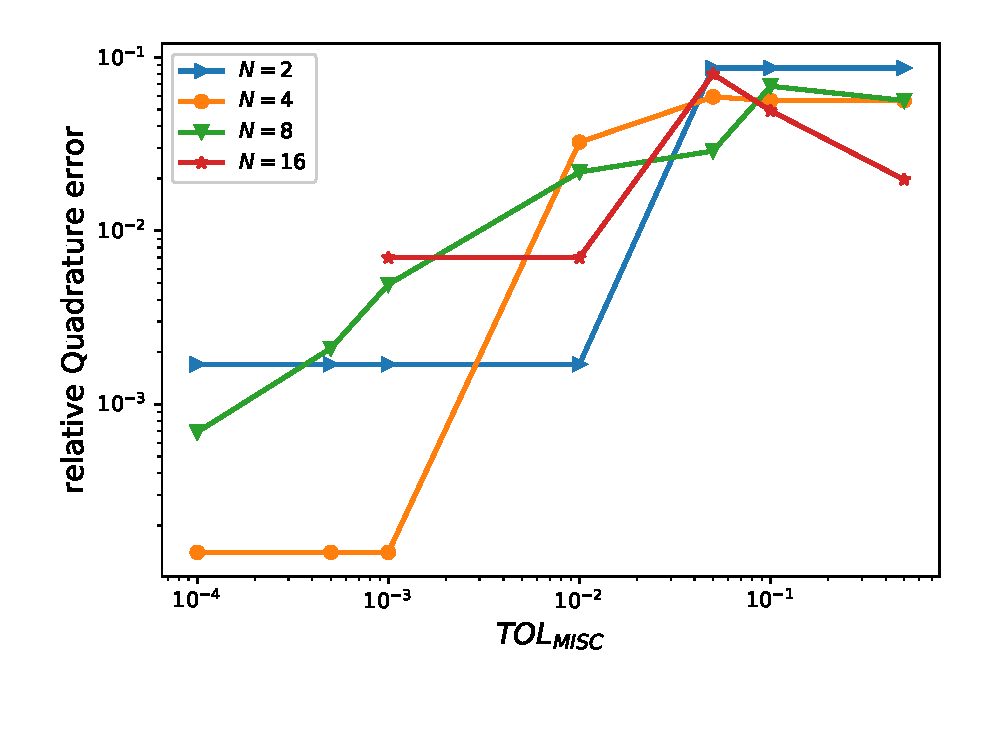
\includegraphics[width=0.5\linewidth]{./figures/rBergomi_MISC_quadratre_error/vs_TOL/set1/relative_quad_error_wrt_MISC_TOL_set1_non_rich}
	
	
	\caption{Quadrature error of MISC, with different tolerances, to compute call option price for different number of time steps. Case  set $1$ parameters, without Richardson extrapolation. See detailed values  in table \ref{Quadrature error of MISC to compute Call option price of the different tolerances for different number of time steps. Case  set $1$ parameters, without Richardson extrapolation. The numbers between parentheses are the corresponding absolute errors.}}
	\label{fig:Quadrature_error_set1}
\end{figure}




\begin{table}[h!]
	\centering
	\begin{tabular}{l*{6}{c}r}
		Method \textbackslash  Steps            & $2$ & $4$ & $8$ & $16$  \\
		\hline
%		MISC ($TOL_{\text{MISC}}=5.10^{-1}$)  & $\mathbf{0.6010}$ & $\mathbf{0.3496}$ & $\mathbf{ 0.2114}$ & $\mathbf{ 0.0974}$  \\
		MISC ($TOL_{\text{MISC}}=10^{-1}$)  & $\mathbf{0.6010}$ & $\mathbf{0.3496}$ & $\mathbf{  0.2232}$ & $\mathbf{
			0.1269}$  \\
%		MISC ($TOL_{\text{MISC}}=5.10^{-2}$)  &$\mathbf{0.6010}$ & $\mathbf{  0.3524}$ & $\mathbf{ 0.1839}$ & $\mathbf{  0.1577}$  \\
		MISC ($TOL_{\text{MISC}}=10^{-2}$)  & $\mathbf{\red{0.5159}}$ & $\mathbf{0.3257}$ & $\mathbf{ 0.1769}$ & $\mathbf{  \red{0.0847}}$  \\
		MISC ($TOL_{\text{MISC}}=10^{-3}$)  & $\mathbf{0.5159}$ & $\mathbf{\red{0.2934}}$ & $\mathbf{0.1600}$ & $\mathbf{0.0847}$  \\
%		MISC ($TOL_{\text{MISC}}=5.10^{-4}$)  & $\mathbf{0.5159}$ & $\mathbf{0.2934}$ & $\mathbf{0.1572}$ & $\mathbf{-}$  \\
		MISC ($TOL_{\text{MISC}}=10^{-4}$)  & $\mathbf{0.5159}$ & $\mathbf{0.2934}$ & $\mathbf{\red{0.1558}}$ & $\mathbf{-}$  \\
		\hline
		MC     & $\mathbf{\red{0.5159}}$ & $\mathbf{\red{0.2938}}$ & $\mathbf{\red{0.1555}}$ &$\mathbf{  \red{0.0817}}$  \\	
		
		\hline
	\end{tabular}
	\caption{Total relative error of MISC, with different tolerances,  and MC to compute call option price for different number of time steps. Case  set $1$ parametrs of table \ref{table:Reference solution, using MC with $500$ time steps, of Call option price under rBergomi model, for different parameter constellation.}, without Richardson extrapolation. The values marked in red, for MISC method, correspond to the total relative errors associated with  stable quadrature errors for MISC, and will be used for complexity comparison against MC.}
	\label{Total error of MISC and MC to compute Call option price of the different tolerances for different number of time steps. Case set 1, without Richardson extrapolation. The numbers between parentheses are the corresponding absolute errors.}
\end{table}



\begin{table}[h!]
	\centering
	\begin{tabular}{l*{6}{c}r}
		Method \textbackslash  Steps            & $2$ & $4$ & $8$ & $16$ &   \\
		\hline
%		MISC ($TOL_{\text{MISC}}=5.10^{-1}$)  & $0.1$ & $0.1$ & $0.2$ & $0.4$  \\
		MISC ($TOL_{\text{MISC}}=10^{-1}$)  & $0.1$ & $0.1$ & $0.6$ & $6$  \\
%		MISC ($TOL_{\text{MISC}}=5.10^{-2}$)  & $0.1$ & $0.3$ & $2$ & $14$  \\
		MISC ($TOL_{\text{MISC}}=10^{-2}$)  & $\red{0.2}$ & $1$ & $9$ & $\red{215}$  \\
		MISC ($TOL_{\text{MISC}}=10^{-3}$)  & $2$ & $\red{11}$ & $243$ & $4650$  \\
%		MISC ($TOL_{\text{MISC}}=5.10^{-4}$)  & $3$ & $17$ & $ 670$ & $-$  \\
		MISC ($TOL_{\text{MISC}}=10^{-4}$)  & $6$ & $96$ & $\red{5760}$ & $-$  \\
		\hline
		MC     & $\red{ 50}$  & $\red{344}$  & $\red{637}$ & $\red{8}$  \\
		
		\hline
		Ratio of $\left(\text{MC}/ \text{MISC} \right)$  &$\red{  250}$ & $\red{    31
		}$  & $\red{ 0.1
		}$  & $\red{  0.04}$ \\
		\hline
	\end{tabular}
	\caption{Comparison of the computational time (in Seconds) of  MC and MISC, used to compute call option price of rBergomi model for different number of time steps. Case set $1$ parametrs of table \ref{table:Reference solution, using MC with $500$ time steps, of Call option price under rBergomi model, for different parameter constellation.}. The
		average MC CPU time is computed over 10 runs. }
	\label{Comparison of the computational time of  MC and MISC, used to compute Call option price of rBergomi model for different number of time steps. Case set1}
\end{table}

\subsubsection*{With Richardson extrapolation (level $1$)}







\begin{table}[h!]
	\centering
	\begin{tabular}{l*{6}{c}r}
		Method \textbackslash  Steps    &$1-2$         & $2-4$ & $4-8$ \\
		\hline
%		MISC ($TOL_{\text{MISC}}=5.10^{-1}$)& $0.1357$  & $0.0783$ & $0.0735$ \\
		MISC ($TOL_{\text{MISC}}=10^{-1}$)  &$0.1357$  &$0.0783$ & $0.0785$   \\
%		MISC ($TOL_{\text{MISC}}=5.10^{-2}$)  & $0.1357$ & $0.0831$ & $0.0773$   \\
		MISC ($TOL_{\text{MISC}}=10^{-2}$)  & $0.1237$ &$0.0781$ & $0.0745$   \\

		MISC ($TOL_{\text{MISC}}=10^{-3}$)  & $0.1224$ &$0.0766$ & $0.0720$  \\
		MISC ($TOL_{\text{MISC}}=10^{-4}$)  &$0.1224$ & $0.0763$ & $0.0724$ \\
		\hline
		MC method ($M=10^6$)  &$	0.1237$ & $0.0752$ & $0.0721$ \\
		\hline
	\end{tabular}
	\caption{Call option price of the different methods for different number of time steps. Case set $1$ parameters of table \ref{table:Reference solution, using MC with $500$ time steps, of Call option price under rBergomi model, for different parameter constellation.}, using Richardson extrapolation (level $1$).}
	\label{table:  Call option price of the different methods for different number of time steps. Case set $1$ parameter, using Richardson extrapolation (level $1$)}
\end{table}




\begin{table}[h!]
	\centering
	\begin{tabular}{l*{6}{c}r}
		Method \textbackslash  Steps            & $1-2$ & $2-4$ & $4-8$ & $8-16$  \\
		\hline
		MC  Bias ($M=10^6$)    &$\underset{( 0.0525)}{\mathbf{0.7378}}$  & $\underset{(    0.0040)}{\mathbf{0.0561}}$  & $\underset{(0.0009 )}{\mathbf{0.0127}}$  & $\underset{(0.0001)}{\mathbf{0.0021}}$ \\	
		
		MC Statistical error ($M=10^6$)   & $\underset{( 2.3e-04)}{\mathbf{3.3e-03}}$  & $\underset{(  1.1e-04)}{\mathbf{1.6e-03}}$  & $\underset{(7.1e-05)}{\mathbf{1.0e-03}}$ & $\underset{(   6.4e-05 )}{\mathbf{9.0e-04}}$ \\	
		
		
		\hline
	\end{tabular}
	\caption{Bias and statistical errors of MC   for computing call option price  for different number of time steps. Case set $1$ parameters in tabel \ref{table:Reference solution, using MC with $500$ time steps, of Call option price under rBergomi model, for different parameter constellation.}, with Richardson extrapolation (level $1$). The numbers between parentheses are the corresponding absolute errors.}
	\label{Bias and Statistical errors of MC ($M=10^6$)  for computing Call option price  for different number of time steps. Case set $1$ parameters, with Richardson extrapolation (level1). The numbers between parentheses are the corresponding absolute errors.}
\end{table}








\begin{figure}[h!]
	\centering
	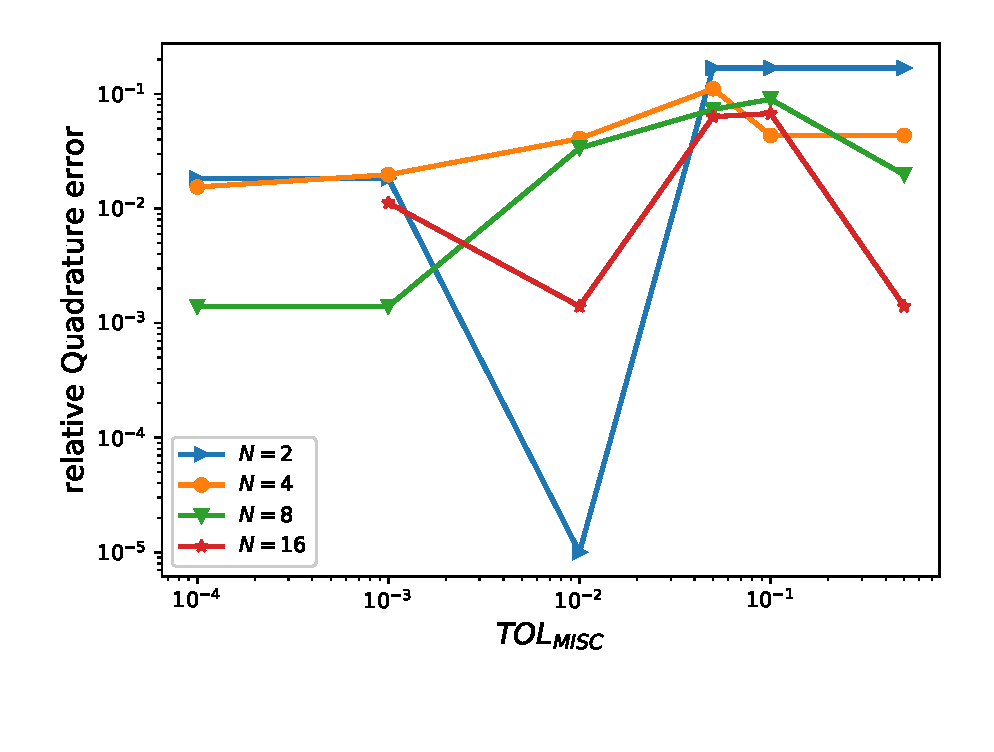
\includegraphics[width=0.5\linewidth]{./figures/rBergomi_MISC_quadratre_error/vs_TOL/set1/relative_quad_error_wrt_MISC_TOL_set1_with_rich}
	
	
	\caption{Quadrature error of MISC, with different tolerances, to compute call option price for different number of time steps. Case  set $1$ parameters, with Richardson extrapolation.  See detailed values  in table \ref{Quadrature error of MISC to compute Call option price of the different tolerances for different number of time steps. Case set $1$ parameters, with Richardson extrapolation(level $1$). The numbers between parentheses are the corresponding absolute errors.}.}
\end{figure}



\begin{table}[!h]
	\centering
	\begin{tabular}{l*{6}{c}r}
		Method \textbackslash  Steps            & $1-2$ & $2-4$ & $4-8$   \\
		\hline
%		MISC ($TOL_{\text{MISC}}=5.10^{-1}$)  & $\mathbf{0.9063
%		}$ & $\mathbf{ 0.0996}$ & $\mathbf{0.0324
%		}$  \\
		MISC ($TOL_{\text{MISC}}=10^{-1}$)  & $\mathbf{0.9063
		}$ & $\mathbf{ 0.0996}$ & $\mathbf{  0.1026}$   \\
%		MISC ($TOL_{\text{MISC}}=5.10^{-2}$)  & $\mathbf{0.9063
%		}$ & $\mathbf{    0.1670}$ & $\mathbf{ 0.0857}$  \\
		MISC ($TOL_{\text{MISC}}=10^{-2}$)  & $\mathbf{0.7378}$ & $\mathbf{  0.0968}$ & $\mathbf{   0.0464}$  \\	
		MISC ($TOL_{\text{MISC}}=10^{-3}$)  & $\mathbf{\red{0.7561}}$ & $\mathbf{\red{0.0758}}$ & $\mathbf{\red{0.0141}}$  \\
		MISC ($TOL_{\text{MISC}}=10^{-4}$)  & $\mathbf{0.7561}$ & $\mathbf{0.0715}$ & $\mathbf{0.0141}$ \\
		\hline
		MC   & $\mathbf{\red{0.7561}}$  & $\mathbf{\red{0.0758}}$  & $\mathbf{\red{0.0141}}$  \\
		
		\hline
	\end{tabular}
	\caption{Total  relative error of MISC and MC, with different tolerances, to compute call option price for different number of time steps. Case set $1$ parameters in table \ref{table:Reference solution, using MC with $500$ time steps, of Call option price under rBergomi model, for different parameter constellation.}, with Richardson extrapolation(level $1$). The values marked in red, for MISC method, correspond to the total relative errors associated with  stable quadrature errors for MISC, and will be used for complexity comparison against MC.}
	\label{Total  error of MISC and MC to compute Call option price of the different tolerances for different number of time steps. Case set $1$ parameters, with Richardson extrapolation(level $1$). The numbers between parentheses are the corresponding absolute errors.}
\end{table}

\begin{table}[!h]
	\centering
	\begin{tabular}{l*{6}{c}r}
		Method \textbackslash  Steps            & $1-2$ & $2-4$ & $4-8$   \\
		\hline
%		MISC ($TOL_{\text{MISC}}=5.10^{-1}$)  & $0.1$ & $0.1$ & $0.2$  \\
		MISC ($TOL_{\text{MISC}}=10^{-1}$)  & $0.1$ & $0.1$ & $0.6$ \\
%		MISC ($TOL_{\text{MISC}}=5.10^{-2}$)  & $0.1$ & $0.4$ & $2$   \\
		MISC ($TOL_{\text{MISC}}=10^{-2}$)  & $1$ & $2$ & $18$   \\
		MISC ($TOL_{\text{MISC}}=10^{-3}$)  & $\red{4}$ & $\red{12}$ & $\red{520}$   \\	
		MISC ($TOL_{\text{MISC}}=10^{-4}$)  & $7$ & $191$ & $7650$  \\
		\hline
		MC   & $\red{ 34.7}$  & $\red{37}$  & $ \red{532}$    \\
		
		\hline
		Ratio of $\left(\text{MC}/ \text{MISC} \right)$  &$\red{8.7}$ & $\red{   3.1
		}$  & $\red{1}$ \\
		\hline
	\end{tabular}
	\caption{Comparison of the computational time (in Seconds) of  MC and MISC, using Richardson extrapolation (level $1$), used to compute call option price of rBergomi model for different number of time steps. Case set $1$ parameters in table \ref{table:Reference solution, using MC with $500$ time steps, of Call option price under rBergomi model, for different parameter constellation.}. The
		average MC CPU time is computed over 10 runs.}
	\label{Comparsion of the computational time of  MC and MISC, using Richardson extrapolation (level $1$), used to compute Call option price of rBergomi model for different number of time steps. Case set $1$ parameters}
\end{table}



\begin{figure}[h!]
	\centering
	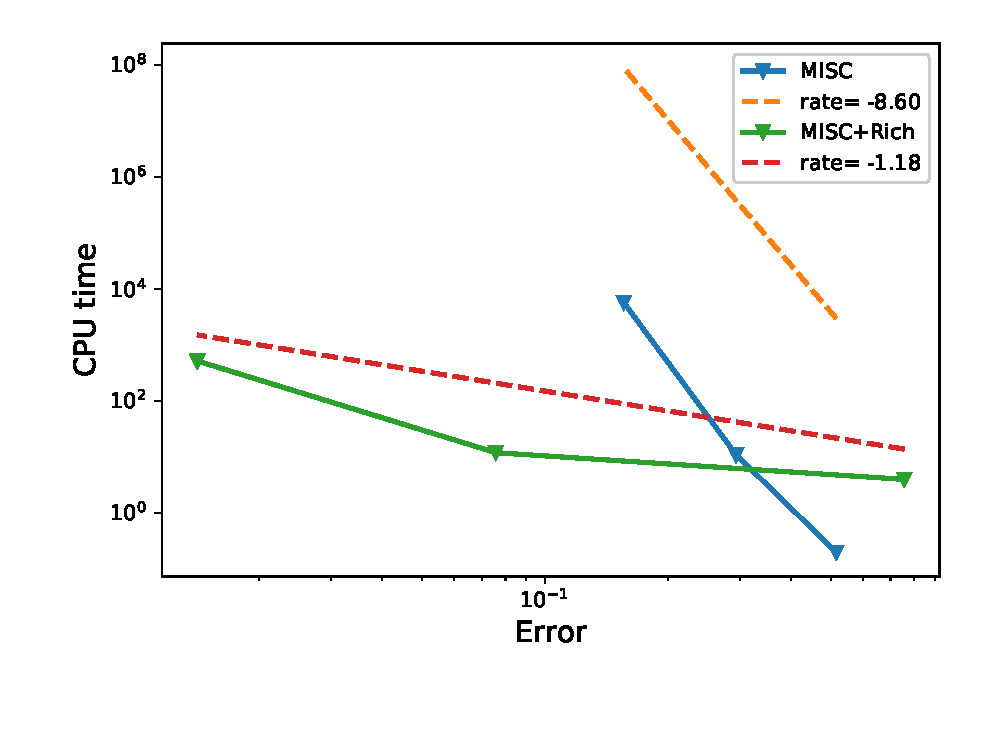
\includegraphics[width=0.5\linewidth]{./figures/rBergomi_Complexity_rates/set1/error_vs_time_set1_comparison}
	
	\caption{Complexity plot for  MISC (with/without) Richardson extrapolation for case set $1$ parameters of table \ref{table:Reference solution, using MC with $500$ time steps, of Call option price under rBergomi model, for different parameter constellation.}.}
	\label{fig:Complexity plot for  MISC for Case set $1$ parameters, comparison}
\end{figure}
\FloatBarrier

\subsubsection*{With Richardson extrapolation (level $2$)}
\begin{table}[h!]
	\centering
	\begin{tabular}{l*{6}{c}r}
		Method \textbackslash  Steps           &$1-2-4$ & $2-4-8$ \\
		\hline
%		MISC ($TOL_{\text{MISC}}=5.10^{-1}$)& $0.0591$  & $0.0719$ \\
		
		MISC ($TOL_{\text{MISC}}=10^{-1}$)  &$0.0567$  &$0.0747$   \\
%		MISC ($TOL_{\text{MISC}}=5.10^{-2}$)  & $0.0733$ & $0.0782$  \\
		MISC ($TOL_{\text{MISC}}=10^{-2}$)  & $		0.0639$ & $0.0729$   \\
		MISC ($TOL_{\text{MISC}}=5.10^{-3}$)  & $	0.0620$ & $0.0708$   \\
		MISC ($TOL_{\text{MISC}}=10^{-3}$)  & $	0.0608$ & $0.0708$  \\
		MISC ($TOL_{\text{MISC}}=10^{-4}$)  & $	0.0608$ & $-$   \\
		\hline
		MC ($M=3.10^6$)  & $0.0608$ & $0.0710$   \\
		\hline 
	\end{tabular}
	\caption{ Call option price of the different methods for different number of time steps.  Case set $1$ parameters in table \ref{table:Reference solution, using MC with $500$ time steps, of Call option price under rBergomi model, for different parameter constellation.}, using Richardson extrapolation (level $2$).}
	\label{table: Call option price of the different methods for different number of time steps. Case $K=1$, using Richardson extrapolation_level2}
\end{table}




\begin{table}[h!]
	\centering
	\begin{tabular}{l*{6}{c}r}
		Method \textbackslash  Steps            & $1-2-4$ & $2-4-8$  \\
		\hline
		MC  Bias ($M=3.10^6$)     &$\underset{( 0.0104)}{\mathbf{ 0.1459}}$  & $\underset{(    1.7e-04)}{\mathbf{0.0024}}$   \\	
		
		MC Statistical error ($M=3.10^6$)   & $\underset{( 1.0e-04)}{\mathbf{1.5e-03}}$  & $\underset{(   4.8e-05)}{\mathbf{    6.8e-04}}$  \\	
		
		
		
		\hline
	\end{tabular}
	\caption{Bias and statistical errors of MC   for computing call option price  for different number of time steps. Case set $1$ parameters in tabel \ref{table:Reference solution, using MC with $500$ time steps, of Call option price under rBergomi model, for different parameter constellation.}, with Richardson extrapolation (level $2$). The numbers between parentheses are the corresponding absolute errors.}
	\label{Bias and Statistical errors of MC ($M=3.10^6$)  for computing Call option price  for different number of time steps. Case set $1$ parameters, with Richardson extrapolation (level2). The numbers between parentheses are the corresponding absolute errors.}
\end{table}





\begin{figure}[h!]
	\centering
	evel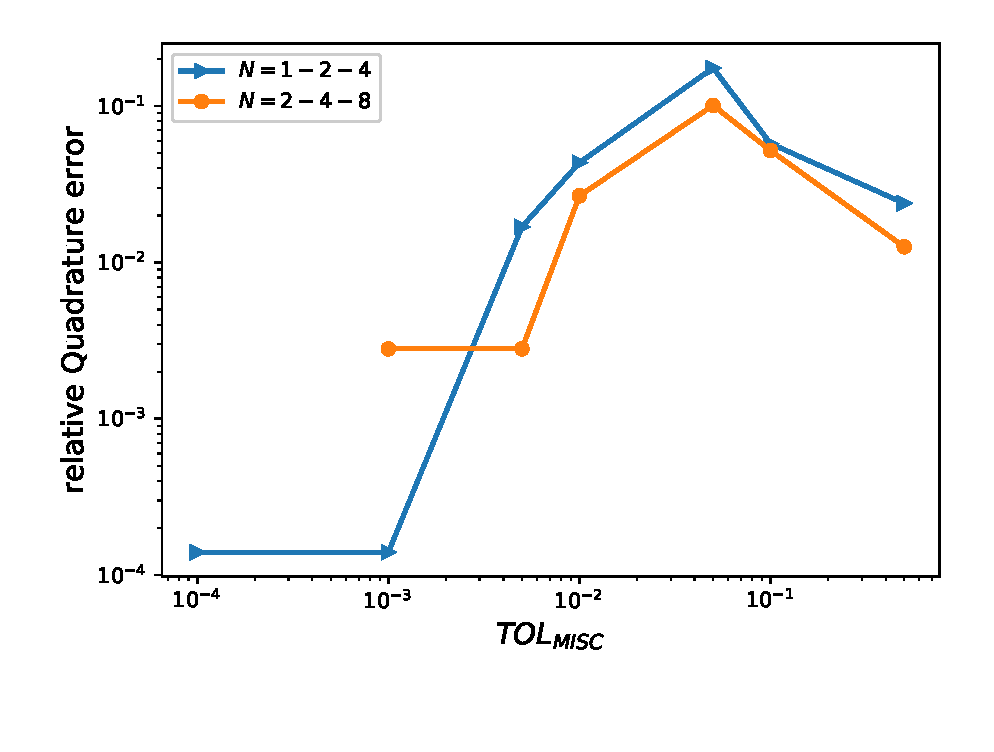
\includegraphics[width=0.5\linewidth]{./figures/rBergomi_MISC_quadratre_error/vs_TOL/set1/relative_quad_error_wrt_MISC_TOL_set1_rich_level2}
	
	
	\caption{Quadrature error of MISC, with different tolerances, to compute call option price of the different tolerances for different number of time steps. Case  set $1$ parameters, with Richardson extrapolation (level $2$).  See detailed values  in table \ref{Quadrature error of MISC to compute Call option price of the different tolerances for different number of time steps. Case set $1$ parameters, with Richardson extrapolation(level $2$). The numbers between parentheses are the corresponding absolute errors.}.}
	\label{fig:Quadrature_error_set1_rich_level2}
\end{figure}




\begin{table}[!h]
	\centering
	\begin{tabular}{l*{6}{c}r}
		Method \textbackslash  Steps            & $1-2-4$ & $2-4-8$  \\
		\hline
%		MISC ($TOL_{\text{MISC}}=5.10^{-1}$)  & $\mathbf{0.1698
%		}$ & $\mathbf{ 0.0150}$  \\
		MISC ($TOL_{\text{MISC}}=10^{-1}$)  & $\mathbf{0.2035
		}$ & $\mathbf{ 0.0544}$ \\
%		MISC ($TOL_{\text{MISC}}=5.10^{-2}$)  & $\mathbf{0.3214
%		}$ & $\mathbf{    0.1035}$  \\
		MISC ($TOL_{\text{MISC}}=10^{-2}$)  & $\mathbf{0.1894}$ & $\mathbf{  0.0291}$   \\	
		MISC ($TOL_{\text{MISC}}=5.10^{-3}$)  & $\mathbf{\red{0.1628}}$ & $\mathbf{\red{0.0052}}$   \\
		MISC ($TOL_{\text{MISC}}=10^{-3}$)  & $\mathbf{0.1460}$ & $\mathbf{0.0052}$   \\
		MISC ($TOL_{\text{MISC}}=10^{-4}$)  & $\mathbf{0.1460}$ & $\mathbf{-}$  \\
		\hline
		MC   & $\mathbf{\red{0.1628}}$  & $\mathbf{\red{0.0052}}$    \\
		\hline
	\end{tabular}
	\caption{Total  relative error of MISC, with different tolerances, and MC to compute call option price for different number of time steps. Case set $1$ parameters in table \ref{table:Reference solution, using MC with $500$ time steps, of Call option price under rBergomi model, for different parameter constellation.}, with Richardson extrapolation(level $2$). The values marked in red, for MISC method, correspond to the total relative errors associated with  stable quadrature errors for MISC, and will be used for complexity comparison against MC.}
	\label{Total  error of MISC and MC to compute Call option price of the different tolerances for different number of time steps. Case set $1$ parameters, with Richardson extrapolation(level $2$). The numbers between parentheses are the corresponding absolute errors.}
\end{table}

\FloatBarrier

\begin{table}[!h]
	\centering
	\begin{tabular}{l*{6}{c}r}
		Method \textbackslash  Steps            & $1-2-4$ & $2-4-8$   \\
		\hline
%		MISC ($TOL_{\text{MISC}}=5.10^{-1}$)  & $0.2$ & $0.3$  \\
		MISC ($TOL_{\text{MISC}}=10^{-1}$)  & $0.25$ & $2$ &   \\
%		MISC ($TOL_{\text{MISC}}=5.10^{-2}$)  & $0.55$ & $5$  \\
		MISC ($TOL_{\text{MISC}}=10^{-2}$)  & $2$ & $24$   \\
		MISC ($TOL_{\text{MISC}}=5.10^{-3}$)  & $\red{5}$ & $\red{64}$  \\	
		MISC ($TOL_{\text{MISC}}=10^{-3}$)  & $24$ & $1067$  \\	
		MISC ($TOL_{\text{MISC}}=10^{-4}$)  & $ 233$ & $-$   \\
		\hline
		MC    & $\red{20}$  & $\red{231}$  \\
		
		\hline
		Ratio of $\left(\text{MC}/ \text{MISC} \right)$  &$\red{4}$ & $\red{  3.6}$   \\
		\hline
	\end{tabular}
	\caption{Comparsion of the computational time (in Seconds) of  MC and MISC, using Richardson extrapolation (level $2$), used to compute call option price of rBergomi model for different number of time steps. Case set $1$ parameters in table \ref{table:Reference solution, using MC with $500$ time steps, of Call option price under rBergomi model, for different parameter constellation.}. The
		average MC CPU time is computed over 10 runs.}
	\label{Comparsion of the computational time of  MC and MISC, using Richardson extrapolation (level $2$), used to compute Call option price of rBergomi model for different number of time steps. Case set $1$ parameters}
\end{table}
















\subsubsection{Case of set $2$ parameters in table \ref{table:Reference solution, using MC with $500$ time steps, of Call option price under rBergomi model, for different parameter constellation.} }
\label{sec:Case of set $2$ parameters_linear}

\subsubsection*{Without Richardson extrapolation}
\begin{table}[h!]
	\centering
	\begin{tabular}{l*{6}{c}r}
		Method \textbackslash  Steps            & $2$ & $4$ & $8$  \\
		\hline
%		MISC ($TOL_{\text{MISC}}=5.10^{-1}$)  & $0.1097$ & $0.0926$ & $0.0807$  \\
		MISC ($TOL_{\text{MISC}}=10^{-1}$)  &$0.1097$ & $0.0926$ & $0.0791$   \\
%		MISC ($TOL_{\text{MISC}}=5.10^{-2}$)  & $0.1097$ & $0.0890$ & $0.0849$  \\
		MISC ($TOL_{\text{MISC}}=10^{-2}$)  & $0.1119$&  $0.1023$ & $0.0910$  \\
		MISC ($TOL_{\text{MISC}}=10^{-3}$)        & $0.1195$ &$0.1023$ &   $0.0910$  \\
		MISC ($TOL_{\text{MISC}}=10^{-4}$)        & $0.1218$ &$0.1023$ &  $-$  \\
		\hline
		MC method ($M=8.10^{6}$)   & $0.1218 $  & $0.1024 $  & $0.0914$  \\		
		\hline
	\end{tabular}
	\caption{ Call option price of the different methods for different number of time steps. Case of set $2$ parameters in table \ref{table:Reference solution, using MC with $500$ time steps, of Call option price under rBergomi model, for different parameter constellation.}, without Richardson extrapolation.}
	\label{table: Call option price of the different methods for different number of time steps. Case set 2_linear}
\end{table}



\begin{table}[h!]
	\centering
	\begin{tabular}{l*{6}{c}r}
		Method \textbackslash  Steps            & $2$ & $4$ & $8$ & $16$  \\
		\hline
		MC Bias ($M=8.10^6$)   & $\underset{(0.0426)}{\mathbf{0.5375
		}}$  & $\underset{ (  0.0208)}{\mathbf{0.2922}}$  & $\underset{(  0.0122)}{\mathbf{0.1542}}$ & $\underset{( 0.0058)}{\mathbf{0.0731}}$  \\	
		
		MC Statistical error ($M=8.10^6$)  & $\underset{( 2.0e-04)}{\mathbf{2.5e-03}}$  & $\underset{(  1.0e-04)}{\mathbf{1.3e-03}}$  & $\underset{(  5.0e-05)}{\mathbf{6.3e-04}}$ & $\underset{(  1.1e-04)}{\mathbf{1.33e-03}}$ \\	
	
		\hline
	\end{tabular}
	\caption{Bias and statistical errors of MC  for computing call option price  for different number of time steps. Case set $2$ parameters in table \ref{table:Reference solution, using MC with $500$ time steps, of Call option price under rBergomi model, for different parameter constellation.}, without Richardson extrapolation. The numbers between parentheses are the corresponding absolute errors.}
	\label{Bias and Statistical errors of MC ($M=10^6$)  for computing Call option price  for different number of time steps. Case set $2$ parameters, without Richardson extrapolation. The numbers between parentheses are the corresponding absolute errors.}
\end{table}





\begin{figure}[h!]
	\centering
	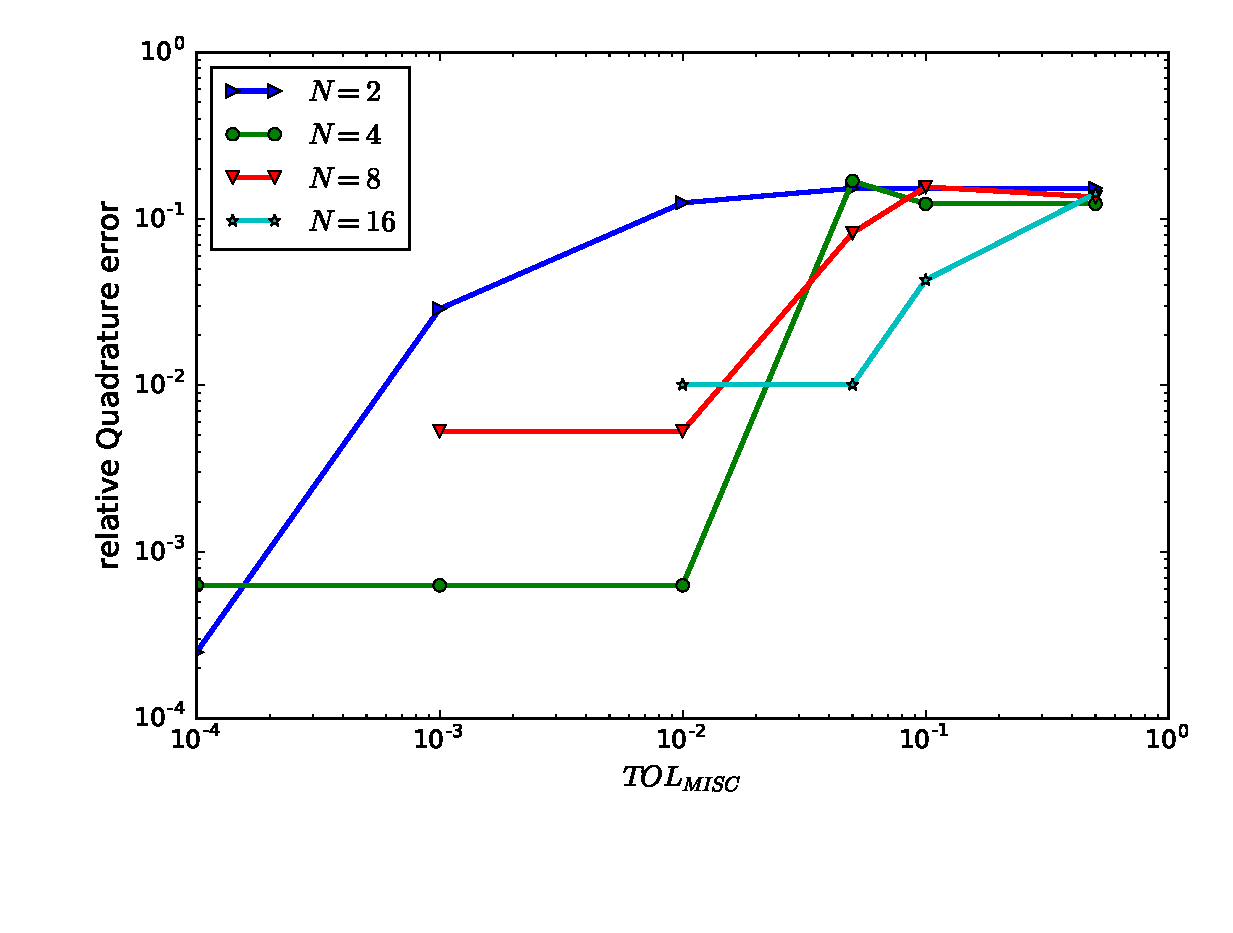
\includegraphics[width=0.5\linewidth]{./figures/rBergomi_MISC_quadratre_error/vs_TOL/set2/relative_quad_error_wrt_MISC_TOL_set2_non_rich_linear}
	
	
	\caption{Quadrature error of MISC, with different tolerances, to compute call option price  of time steps. Case  set $2$ parameters, without Richardson extrapolation.  See detailed values  in table \ref{Quadrature error of MISC to compute Call option price of the different tolerances for different number of time steps. Case  set $2$ parameters, without Richardson extrapolation. The numbers between parentheses are the corresponding absolute errors,linear}.}
	\label{fig:Quadrature_error_set2_linear}
\end{figure}

\FloatBarrier
\begin{table}[h!]
	\centering
	\begin{tabular}{l*{6}{c}r}
		Method \textbackslash  Steps            & $2$ & $4$ & $8$   \\
		\hline
%		MISC ($TOL_{\text{MISC}}=5.10^{-1}$)  & $\mathbf{
%			0.6900}$ & $\mathbf{   
%			0.4153
%		}$ & $\mathbf{    0.2895}$   \\
		MISC ($TOL_{\text{MISC}}=10^{-1}$)  & $\mathbf{
			0.6900}$& $\mathbf{    
			0.4153}$ & $\mathbf{     
			0.3097
		}$   \\
%		MISC ($TOL_{\text{MISC}}=5.10^{-2}$)  &$\mathbf{
%			0.6900}$ & $\mathbf{         0.4608
%		}$ & $\mathbf{      
%			0.2365
%		}$ \\
		MISC ($TOL_{\text{MISC}}=10^{-2}$)  & $\mathbf{ 
			0.6622}$ & $\mathbf{  \red{ 
				0.2928
			}
		}$ & $\mathbf{ \red{    0.1595}}$   \\
		MISC ($TOL_{\text{MISC}}=10^{-3}$)        & $\mathbf{
			0.6371}$  &  $\mathbf{
			0.2928
		}$ &  $\mathbf{    0.1595}$ \\
		MISC ($TOL_{\text{MISC}}=10^{-4}$)        & $\mathbf{       \red{0.5378}}$  & $\mathbf{
			0.2928
		}$  &  $-$ \\
		\hline
		MC    & $\mathbf{\red{    0.5400}}$  & $\mathbf{\red{0.2935}
		}$  &$\mathbf{\red{
				0.1593}}$  \\	
		
		\hline
	\end{tabular}
	\caption{Total relative error of MISC, with different tolerances, and MC to compute Call option price  for different number of time steps. Case  set $2$ parameters in table \ref{table:Reference solution, using MC with $500$ time steps, of Call option price under rBergomi model, for different parameter constellation.}, without Richardson extrapolation. The numbers between parentheses are the corresponding absolute errors. The values marked in red, for MISC method, correspond to the total relative errors associated with  stable quadrature errors for MISC, and will be used for complexity comparison against MC.}
	\label{Total error of MISC and MC to compute Call option price of the different tolerances for different number of time steps. Case $K=1$, $H=0.07$, without Richardson extrapolation. The numbers between parentheses are the corresponding absolute errors,linear}
\end{table}

\begin{table}[h!]
	\centering
	\begin{tabular}{l*{6}{c}r}
		Method \textbackslash  Steps            & $2$ & $4$ & $8$   \\
		\hline
%		MISC ($TOL_{\text{MISC}}=5.10^{-1}$)  & $0.08$ & $0.13$ & $0.2$ \\
		MISC ($TOL_{\text{MISC}}=10^{-1}$)  & $0.08$ & $0.13$ & $0.7$   \\
%		MISC ($TOL_{\text{MISC}}=5.10^{-2}$)  & $0.08$ & $0.25$ & $7$   \\
		MISC ($TOL_{\text{MISC}}=10^{-2}$)  & $0.2$& $\red{5}$ & $\red{333}$   \\
		MISC ($TOL_{\text{MISC}}=10^{-3}$)  &  $2$ & $73$ & $3650$  \\		
		MISC ($TOL_{\text{MISC}}=10^{-4}$)  & $\red{43}$ & $1240$ & $-$  \\	
	
		\hline
		MC method & $\red{220}$  & $\red{358}$  & $\red{9}$  \\
		\hline	
		Ratio of $\left(\text{MC}/ \text{MISC} \right)$  &$\red{5}$ & $\red{   72 
		}$  & $\red {  0.03	}$   \\
		\hline
	\end{tabular}
	\caption{Comparison of the computational time (in Seconds) of  MC and MISC, used to compute Call option price of rBergomi model for different number of time steps. Case  set $2$ parameters in table \ref{table:Reference solution, using MC with $500$ time steps, of Call option price under rBergomi model, for different parameter constellation.}. The
		average MC CPU time is computed over 10 runs.}
	\label{Comparsion of the computational time of  MC and MISC, used to compute Call option price of rBergomi model for different number of time steps. Case $K=1, H=0.07$, linear}
\end{table}

\FloatBarrier
\subsubsection*{With Richardson extrapolation (level $1$)}

\begin{table}[h!]
	\centering
	\begin{tabular}{l*{6}{c}r}
		Method \textbackslash  Steps    &$1-2$         & $2-4$ & $4-8$ \\
		\hline
%		MISC ($TOL_{\text{MISC}}=5.10^{-1}$)  &$0.1260$ & $0.0756$ & $0.0687$\\
		MISC ($TOL_{\text{MISC}}=10^{-1}$)  &$0.1260$ & $0.0756$ & $0.0702$   \\
		MISC ($TOL_{\text{MISC}}=5.10^{-2}$)   &$0.1260$ & $0.0716$ & $0.0796$    \\
		MISC ($TOL_{\text{MISC}}=10^{-2}$)  &$0.1456$ & $0.0838$ & $0.0796$  \\	
		MISC ($TOL_{\text{MISC}}=10^{-3}$)  &$0.1497$ & $0.0838$ & $-$ \\
		
		MISC ($TOL_{\text{MISC}}=10^{-4}$)  &$0.1501$ & $-$ & $-$ \\
		\hline
		MC method ($M=10^{6}$)   & $0.1552 $  & $0.0846 $  & $0.0804$  \\		
		\hline
	\end{tabular}
	\caption{Call option price of the different methods for different number of time steps. Case set $2$ parameters of table \ref{table:Reference solution, using MC with $500$ time steps, of Call option price under rBergomi model, for different parameter constellation.}, using Richardson extrapolation (level $1$)}
	\label{table:  Call option price of the different methods for different number of time steps. Case set $2$ parameter, using Richardson extrapolation (level $1$),linear}
\end{table}



\begin{table}[h!]
	\centering
	\begin{tabular}{l*{6}{c}r}
		Method \textbackslash  Steps            & $1-2$ & $2-4$ & $4-8$ & $8-16$  \\
		\hline
		MC Bias ($M=10^6$)  &$\underset{( 0.0760)}{\mathbf{0.9594}}$  & $\underset{( 0.0054)}{\mathbf{0.0686}}$  & $\underset{(   0.0012)}{\mathbf{0.0149}}$  & $\underset{(  0.0004)}{\mathbf{0.0048}}$ \\	
		
		MC Statistical error ($M=10^6$)   & $\underset{( 1e-03)}{\mathbf{1.3e-02}}$  & $\underset{(   3.2e-04)}{\mathbf{4.1e-03}}$  & $\underset{(  1.7e-04)}{\mathbf{2.1e-03}}$ & $\underset{(  1.3e-04)}{\mathbf{1.6e-03}}$ \\	
		\hline
	\end{tabular}
	\caption{Bias and statistical errors of MC   for computing call option price  for different number of time steps. Case set $2$ parameters in tabel \ref{table:Reference solution, using MC with $500$ time steps, of Call option price under rBergomi model, for different parameter constellation.}, with Richardson extrapolation (level $1$). The numbers between parentheses are the corresponding absolute errors.}
	\label{Bias and Statistical errors of MC ($M=10^6$)  for computing Call option price  for different number of time steps. Case set $2$ parameters, with Richardson extrapolation (level1). The numbers between parentheses are the corresponding absolute errors.}
\end{table}








\begin{figure}[h!]
	\centering
	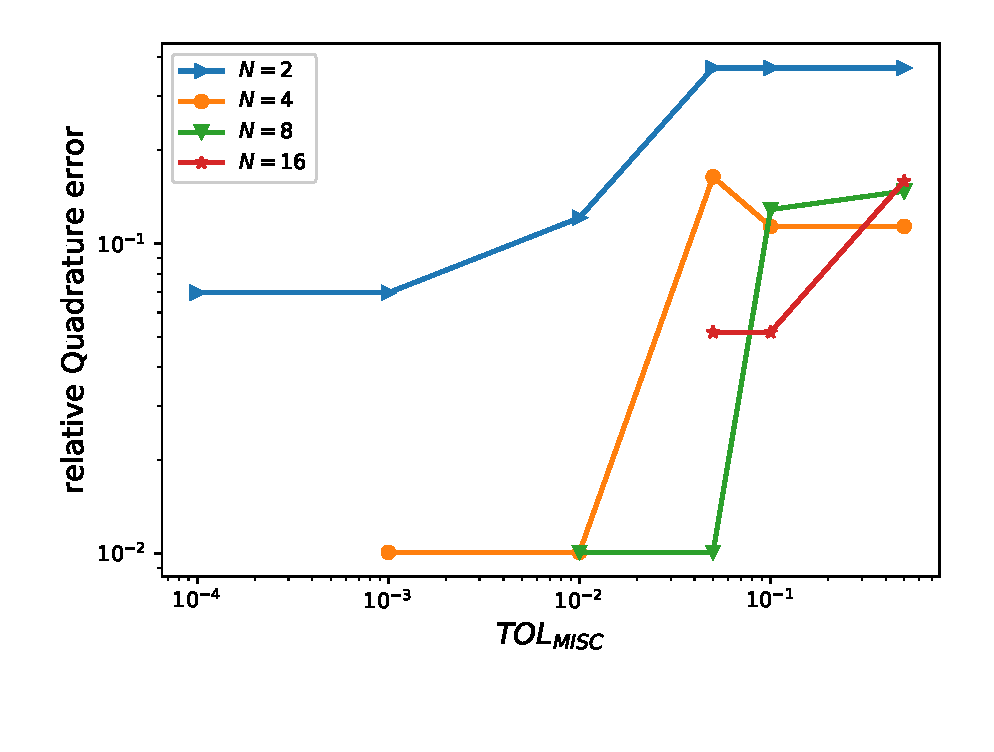
\includegraphics[width=0.5\linewidth]{./figures/rBergomi_MISC_quadratre_error/vs_TOL/set2/relative_quad_error_wrt_MISC_TOL_set2_with_rich_linear}
	
	
	\caption{Quadrature error of MISC, with different tolerances,  to compute call option price for different number of time steps. Case  set $2$ parameters, with Richardson extrapolation.  See detailed values  in table \ref{Quadrature error of MISC to compute Call option price of the different tolerances for different number of time steps. Case set $2$ parameters, with Richardson extrapolation(level $1$). The numbers between parentheses are the corresponding absolute errors,linear}.}
	\label{fig:Quadrature_error_set2_linear_rich}
\end{figure}


\begin{table}[h!]
	\centering
	\begin{tabular}{l*{6}{c}r}
		Method \textbackslash  Steps            & $1-2$ & $2-4$ & $4-8$  \\
		\hline
%		MISC ($TOL_{\text{MISC}}=5.10^{-1}$)  & $\mathbf{  1.3281}$ & $\mathbf{  0.1822}$ & $\mathbf{
%			0.1626
%		}$  \\
		MISC ($TOL_{\text{MISC}}=10^{-1}$)  & $\mathbf{  1.3281}$ & $\mathbf{0.1822}$ & $\mathbf{0.1437}$   \\
		MISC ($TOL_{\text{MISC}}=5.10^{-2}$)  & $\mathbf{  1.3281}$ & $\mathbf{ 0.2327}$ & $\mathbf{  \red{0.0250}}$   \\
		MISC ($TOL_{\text{MISC}}=10^{-2}$)  & $\mathbf{   1.0806
		}$ & $\mathbf{    \red{0.0787}}$ & $\mathbf{ 0.0250}$  \\
		MISC ($TOL_{\text{MISC}}=10^{-3}$)  & $\mathbf{ \red{  1.0288}}$ & $\mathbf{    0.0787}$ & $\mathbf{-}$  \\
		
		MISC ($TOL_{\text{MISC}}=10^{-4}$)  & $\mathbf{     1.0238}$ & $\mathbf{-}$ & $\mathbf{-}$  \\

		\hline
		
		MC &$\mathbf{ \red{  1.0288}}$  & $\mathbf{\red{0.0787}}$ & $\mathbf{\red{0.0250}}$  \\
		
		\hline
	\end{tabular}
	\caption{Total relative error of MISC, with different tolerances,  and MC to compute call option price  for different number of time steps. Case set $2$ parameters in table \ref{table:Reference solution, using MC with $500$ time steps, of Call option price under rBergomi model, for different parameter constellation.}, with Richardson extrapolation(level $1$). The numbers between parentheses are the corresponding absolute errors. The values marked in red, for MISC method, correspond to the total relative errors associated with  stable quadrature errors for MISC, and will be used for complexity comparison against MC.}
	\label{Total  error of MISC and MC to compute Call option price of the different tolerances for different number of time steps. Case set $2$ parameters, with Richardson extrapolation(level $1$). The numbers between parentheses are the corresponding absolute errors,relative}
\end{table}


\begin{table}[h!]
	\centering
	\begin{tabular}{l*{6}{c}r}
		Method \textbackslash  Steps            & $1-2$ & $2-4$ & $4-8$   \\
		\hline
%		MISC ($TOL_{\text{MISC}}=5.10^{-1}$)  & $0.1$ & $0.18$ & $0.3$   \\
		MISC ($TOL_{\text{MISC}}=10^{-1}$)  & $0.1$ & $0.18$ & $1.6$  \\
		MISC ($TOL_{\text{MISC}}=5.10^{-2}$)  & $0.1$ & $0.6$ & $\red{37}$  \\
		MISC ($TOL_{\text{MISC}}=10^{-2}$)  & $1.3$ & $\red{6}$ & $2382$  \\
		MISC ($TOL_{\text{MISC}}=10^{-3}$)  & $\red{3.5}$ & $ 244$ & $-$   \\
		
		MISC ($TOL_{\text{MISC}}=10^{-4}$)  & $140$ & $-$ & $-$ \\
		\hline	
		MC  &$\red{12}$ & $\red{113}$  & $\red{130}$   \\
		
		\hline	
		Ratio of $\left(\text{MC}/ \text{MISC} \right)$  &$\red{ 3.4
		}$ & $\red{     18.8
		}$  & $\red{ 3.5}
		$  \\
		\hline
		\end{tabular}
		\caption{Comparison of the computational time (in Seconds) of  MC and MISC, using Richardson extrapolation (level $1$), used to compute call option price of rBergomi model for different number of time steps. Case set $2$ parameters in table \ref{table:Reference solution, using MC with $500$ time steps, of Call option price under rBergomi model, for different parameter constellation.}. The
			average MC CPU time is computed over 10 runs.}
		\label{Comparsion of the computational time of  MC and MISC, using Richardson extrapolation (level $1$), used to compute Call option price of rBergomi model for different number of time steps. Case set $2$ parameters,linear}
		\end{table}
		
		\FloatBarrier
	\subsubsection*{With Richardson extrapolation (level $2$)}
		

		\begin{table}[h!]
		\centering
		\begin{tabular}{l*{6}{c}r}
		Method \textbackslash  Steps           &$1-2-4$ & $2-4-8$ \\
		\hline
%		MISC ($TOL_{\text{MISC}}=5.10^{-1}$)& $0.0587$  & $0.0664 $ \\
		
		MISC ($TOL_{\text{MISC}}=10^{-1}$)  &$0.0587$  &$ 0.0702$   \\
		MISC ($TOL_{\text{MISC}}=5.10^{-2}$)  & $0.0401$ & $0.0790$  \\
		MISC ($TOL_{\text{MISC}}=10^{-2}$)  & $0.0623$ &  $0.0784$   \\
		MISC ($TOL_{\text{MISC}}=5.10^{-3}$)  & $0.0623$ & $-$   \\
		MISC ($TOL_{\text{MISC}}=10^{-3}$)  & $0.0608$ & $$  \\
		
		\hline
		MC ($M=3.10^6$)  & $ 0.0601$ & $ 0.0787$   \\
		\hline 
	\end{tabular}
	\caption{ Call option price of the different methods for different number of time steps. Case set $2$ parameters in tabel \ref{table:Reference solution, using MC with $500$ time steps, of Call option price under rBergomi model, for different parameter constellation.}, using Richardson extrapolation (level 2).}
	\label{table: Call option price of the different methods for different number of time steps. Case $K=1,H=0.07$, using Richardson extrapolation_level2,linear}
\end{table}




\begin{table}[h!]
	\centering
	\begin{tabular}{l*{6}{c}r}
		Method \textbackslash  Steps            & $1-2-4$ & $2-4-8$  \\
		\hline
		MC  Bias  ($M=3.10^6$)   &$\underset{(  0.0191)}{\mathbf{  0.2411}}$  & $\underset{(      4.6e-04)}{\mathbf{  0.0058}}$   \\	
		
		MC Statistical error ($M=3.10^6$)   & $\underset{( 2.8e-04)}{\mathbf{3.5e-03}}$  & $\underset{(   1.4e-04)}{\mathbf{    1.8e-03}}$  \\	
		
		
		
		\hline
	\end{tabular}
	\caption{Bias and statistical errors of MC   for computing call option price  for different number of time steps. Case set $2$ parameters in tabel \ref{table:Reference solution, using MC with $500$ time steps, of Call option price under rBergomi model, for different parameter constellation.}, with Richardson extrapolation (level $2$). The numbers between parentheses are the corresponding absolute errors.}
	\label{Bias and Statistical errors of MC ($M=3.10^6$)  for computing Call option price  for different number of time steps. Case set $2$ parameters, with Richardson extrapolation (level2). The numbers between parentheses are the corresponding absolute errors.}
\end{table}





\begin{figure}[h!]
	\centering
	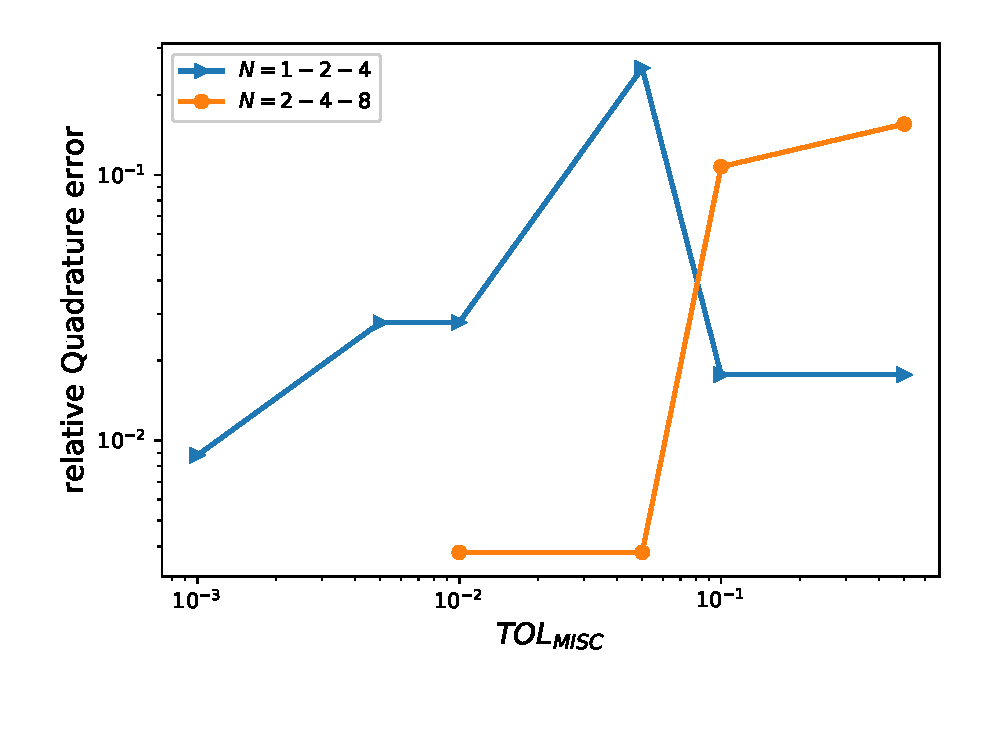
\includegraphics[width=0.5\linewidth]{./figures/rBergomi_MISC_quadratre_error/vs_TOL/set2/relative_quad_error_wrt_MISC_TOL_set2_rich_level2_linear}
	
	
	\caption{Quadrature error of MISC to compute Call option price of the different tolerances for different number of time steps. Case  set $2$ parameters, with Richardson extrapolation (level $2$).  See detailed values  in table \ref{Quadrature error of MISC to compute Call option price of the different tolerances for different number of time steps. Case set $2$ parameters, with Richardson extrapolation(level $2$). The numbers between parentheses are the corresponding absolute errors,linear}.}
	\label{fig:Quadrature_error_set2_rich_linear}
\end{figure}


\begin{table}[!h]
	\centering
	\begin{tabular}{l*{6}{c}r}
		Method \textbackslash  Steps            & $1-2-4$ & $2-4-8$  \\
		\hline
%		MISC ($TOL_{\text{MISC}}=5.10^{-1}$)  & $\mathbf{ 0.2588
%		}$ & $\mathbf{ 0.1611}$  \\
		MISC ($TOL_{\text{MISC}}=10^{-1}$)  & $\mathbf{ 0.2588
		}$ & $\mathbf{ 0.1131}$ \\
		MISC ($TOL_{\text{MISC}}=5.10^{-2}$)  & $\mathbf{   0.4936
		}$ & $\mathbf{\red{ 0.0096} }$  \\
		MISC ($TOL_{\text{MISC}}=10^{-2}$)  & $\mathbf{ \red{0.2689}}$ & $\mathbf{ 0.0096 }$    \\	
		MISC ($TOL_{\text{MISC}}=5.10^{-3}$)  & $\mathbf{ 0.2689}$ & $\mathbf{-}$   \\
		MISC ($TOL_{\text{MISC}}=10^{-3}$)  & $\mathbf{ 0.2499}$ & $\mathbf{-}$   \\
		\hline
		MC   & $\mathbf{\red{0.2689}}$  & $\mathbf{\red{ 0.0096}}$    \\
		\hline
	\end{tabular}
	\caption{Total relative  error of MISC, with different tolerances, and MC to compute call option price   for different number of time steps. Case set $2$ parameters in table \ref{table:Reference solution, using MC with $500$ time steps, of Call option price under rBergomi model, for different parameter constellation.}, with Richardson extrapolation(level $2$). The values marked in red, for MISC method, correspond to the total relative errors associated with  stable quadrature errors for MISC, and will be used for complexity comparison against MC.}
	\label{Total  error of MISC and MC to compute Call option price of the different tolerances for different number of time steps. Case set $2$ parameters, with Richardson extrapolation(level $2$). The numbers between parentheses are the corresponding absolute errors,linear}
\end{table}

\begin{table}[!h]
	\centering
	\begin{tabular}{l*{6}{c}r}
		Method \textbackslash  Steps            & $1-2-4$ & $2-4-8$   \\
		\hline
%		MISC ($TOL_{\text{MISC}}=5.10^{-1}$)  & $0.2$ & $0.4$  \\
		MISC ($TOL_{\text{MISC}}=10^{-1}$)  & $0.2$ & $2$ &   \\
		MISC ($TOL_{\text{MISC}}=5.10^{-2}$)  & $0.5$ & $\red{74}$  \\
		MISC ($TOL_{\text{MISC}}=10^{-2}$)  & $\red{9}$ & $3455$   \\
		MISC ($TOL_{\text{MISC}}=5.10^{-3}$)  & $30$ & $-$  \\	
		MISC ($TOL_{\text{MISC}}=10^{-3}$)  & $693$ & $-$  \\	
		\hline
		MC    & $ \red{  118}$  & $\red{1274}$  \\
		
		\hline
		Ratio of $\left(\text{MC}/ \text{MISC} \right)$  &$\red{13}$ & $\red{  17}$   \\
		\hline
	\end{tabular}
	\caption{Comparison of the computational time (in Seconds) of  MC and MISC, using Richardson extrapolation (level $2$), used to compute call option price of rBergomi model for different number of time steps. Case set $2$ parameters in table \ref{table:Reference solution, using MC with $500$ time steps, of Call option price under rBergomi model, for different parameter constellation.}. The
		average MC CPU time is computed over 10 runs.}
	\label{Comparsion of the computational time of  MC and MISC, using Richardson extrapolation (level $2$), used to compute Call option price of rBergomi model for different number of time steps. Case set $2$ parameters,linear}
\end{table}





\FloatBarrier

\subsubsection{Case of set $3$ parameters in table \ref{table:Reference solution, using MC with $500$ time steps, of Call option price under rBergomi model, for different parameter constellation.}}\label{sec:Case of set 3 parameters}


\subsubsection*{Without Richardson extrapolation}

\begin{table}[h!]
	\centering
	\begin{tabular}{l*{6}{c}r}
		Method \textbackslash  Steps            & $2$ & $4$ & $8$ & $16$ &   \\
		\hline
%		MISC ($TOL_{\text{MISC}}=5.10^{-1}$)  & $0.1258$ & $0.1239$ & $0.1231$ & $0.1227$  \\
		MISC ($TOL_{\text{MISC}}=10^{-1}$)  & $0.1258$ & $0.1239$ & $0.1231$ & $0.1229$  \\
%		MISC ($TOL_{\text{MISC}}=5.10^{-2}$)  & $0.1258$ & $0.1239$ & $0.1231$ & $0.1241$  \\
		MISC ($TOL_{\text{MISC}}=10^{-2}$)  & $0.1258$ & $0.1246$ & $0.1248$ & $0.1250$  \\
		
		MISC ($TOL_{\text{MISC}}=10^{-3}$)  & $0.1271$ & $0.1259$ & $0.1252$ & $0.1249$  \\
		MISC ($TOL_{\text{MISC}}=10^{-4}$)  & $0.1270$ & $0.1258$ & $0.1252$ & $-$  \\
		
			MISC ($TOL_{\text{MISC}}=10^{-5}$)  & $0.1270$ &$0.1258$ &  $0.1252$ & $-$  \\
		\hline
		MC method ($M=3.10^{6}$)   & $    0.1269$ & $0.1257$  & $0.1253$ & $0.1249$ \\		
		
		\hline
	\end{tabular}
	\caption{ Call option price of the different methods for different number of time steps. Case of set $3$ parameters in table \ref{table:Reference solution, using MC with $500$ time steps, of Call option price under rBergomi model, for different parameter constellation.}, without Richardson extrapolation.}
	\label{table: Call option price of the different methods for different number of time steps. Case set 3}
\end{table}


\begin{table}[h!]
	\centering
	\begin{tabular}{l*{6}{c}r}
		Method \textbackslash  Steps            & $2$ & $4$ & $8$ & $16$  \\
		\hline
		MC Bias ($M=3.10^6$)   & 	$ \underset{(    0.0022)}{\mathbf{0.0174}}$  & $\underset{(0.001)}{\mathbf{0.0078}}$  & $\underset{(0.0005)}{\mathbf{0.0042}}$ & $\underset{(0.0001)}{\mathbf{0.0008}}$\\ 
		
		MC Statistical error ($M=3.10^6$)  &  $\underset{(   6.2e-05)} {\mathbf{5.0e-04}}$  & $\underset{(5.9e-05)} {\mathbf{4.7e-04}}$  & $\underset{(5.8e-05)} {\mathbf{4.6e-04 }}$ & $\underset{(5.8e-05)} {\mathbf{4.6e-04 }}$	\\
		
		\hline
	\end{tabular}
	\caption{Bias and statistical errors of MC   for computing call option price  for different number of time steps. Case set $3$, without Richardson extrapolation. The numbers between parentheses are the corresponding absolute errors.}
	\label{Bias and Statistical errors of MC ($M=10^6$)  for computing Call option price  for different number of time steps. Case set 3, without Richardson extrapolation. The numbers between parentheses are the corresponding absolute errors.}
\end{table}






	\begin{figure}[h!]
		\centering
		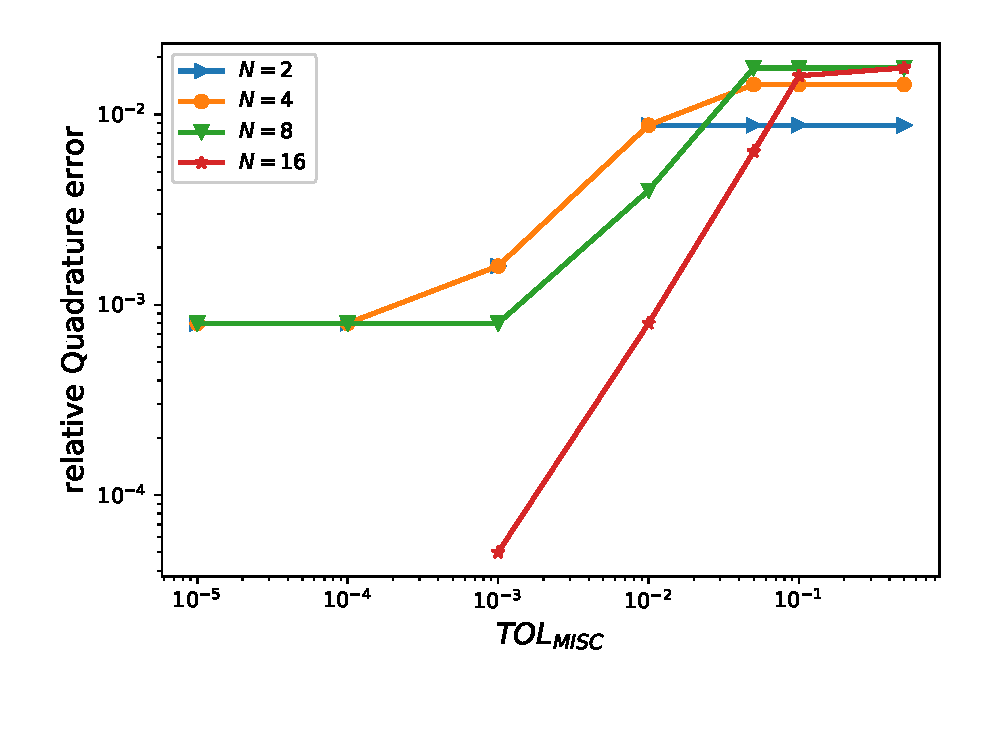
\includegraphics[width=0.5\linewidth]{./figures/rBergomi_MISC_quadratre_error/vs_TOL/set5/relative_quad_error_wrt_MISC_TOL_set5_non_rich}
	
	
	\caption{Quadrature error of MISC, with different tolerances, to compute call option price  for different number of time steps. Case  set $3$ parameters, without Richardson extrapolation.  See detailed values  in table \ref{Quadrature error of MISC to compute Call option price of the different tolerances for different number of time steps. Case  set $3$ parameters, without Richardson extrapolation. The numbers between parentheses are the corresponding absolute errors.}.}
	\label{fig:Quadrature_error_set3}
\end{figure}




\begin{table}[h!]
	\centering
	\begin{tabular}{l*{6}{c}r}
		Method \textbackslash  Steps            & $2$ & $4$ & $8$ & $16$  \\
		\hline
%		MISC ($TOL_{\text{MISC}}=5.10^{-1}$)  & $\mathbf{0.0262}$ & $\mathbf{0.0222}$ & $\mathbf{ 0.0218}$ & $\mathbf{ 0.0184}$  \\
		MISC ($TOL_{\text{MISC}}=10^{-1}$)  &  $\mathbf{0.0262}$ & $\mathbf{0.0222}$& $\mathbf{ 0.0218}$ & $\mathbf{ 0.0168}$   \\
%		MISC ($TOL_{\text{MISC}}=5.10^{-2}$)  & $\mathbf{0.0262}$ & $\mathbf{0.0222}$ & $\mathbf{ 0.0218}$ & $\mathbf{ 0.0072}$  \\
		MISC ($TOL_{\text{MISC}}=10^{-2}$)  &  $\mathbf{0.0262}$ & $\mathbf{0.0166}$& $\mathbf{ 0.0082}$ & $\mathbf{ \red{0.0016}}$  \\
		MISC ($TOL_{\text{MISC}}=10^{-3}$)  &  $\mathbf{0.0190}$ & $\mathbf{0.0094}$& $\mathbf{\red{0.0050}}$  & $\mathbf{ 0.0008}$  \\
		MISC ($TOL_{\text{MISC}}=10^{-4}$)  &  $\mathbf{\red{0.0182}}$ & $\mathbf{\red{0.0086}}$& $\mathbf{0.0050}$ & $\mathbf{ -}$ \\
			MISC ($TOL_{\text{MISC}}=10^{-5}$)  &  $\mathbf{0.0182}$ & $\mathbf{0.0086}$& $\mathbf{0.0050}$ & $\mathbf{ -}$ 
			 \\
		\hline
		MC    & $\mathbf{\red{0.0179}}$  & $\mathbf{ \red{0.0083}}$  & $\mathbf{\red{0.0047}}$ & $\mathbf{ \red{0.0013}}$  \\		
		\hline
	\end{tabular}
	\caption{Total relative error of MISC, with different tolerances, and MC to compute call option price for different number of time steps. Case set $3$ parametrs of table \ref{table:Reference solution, using MC with $500$ time steps, of Call option price under rBergomi model, for different parameter constellation.}, without Richardson extrapolation. The numbers between parentheses are the corresponding absolute errors. The values marked in red, for MISC method, correspond to the total relative errors associated with  stable quadrature errors for MISC, and will be used for complexity comparison against MC.}
	\label{Total error of MISC and MC to compute Call option price of the different tolerances for different number of time steps. Case set 3, without Richardson extrapolation. The numbers between parentheses are the corresponding absolute errors.}
\end{table}



\begin{table}[h!]
	\centering
	\begin{tabular}{l*{6}{c}r}
		Method \textbackslash  Steps            & $2$ & $4$ & $8$ & $16$ &   \\
		\hline
%		MISC ($TOL_{\text{MISC}}=5.10^{-1}$)  & $0.1$ & $0.1$ & $0.2$ & $0.4$  \\
		MISC ($TOL_{\text{MISC}}=10^{-1}$)  & $0.1$ & $0.1$ & $0.2$ & $0.8$ \\
%		MISC ($TOL_{\text{MISC}}=5.10^{-2}$)  & $0.1$ & $0.1$ & $0.2$ & $22$  \\
		MISC ($TOL_{\text{MISC}}=10^{-2}$)  & $0.1$ & $0.5$ & $8$ & $\red{92}$ \\
		MISC ($TOL_{\text{MISC}}=10^{-3}$)  & $0.5$ & $3$ & $\red{24}$ & $2226$ \\
		MISC ($TOL_{\text{MISC}}=10^{-4}$)  & $\red{1}$ & $\red{6}$ & $80$ & $-$\\
		MISC ($TOL_{\text{MISC}}=10^{-5}$)  & $2$ & $32$ & $1760$ & $-$
		 \\
		\hline
		MC method   & $ \red{122}
		
		$  & $  \red{211}$  & $  \red{427}$ & $ \red{766}
		$  \\	
		\hline
		Ratio of $\left(MC/MISC \right)$ & $ \red{122}
		
		$  & $  \red{35}$  & $  \red{  18
		}$ & $ \red{ 8}
		$  \\	
		
		\hline
	\end{tabular}
	\caption{Comparison of the computational time (in Seconds) of  MC and MISC, used to compute Call option price of rBergomi model for different number of time steps. Case set $3$ parametrs of table \ref{table:Reference solution, using MC with $500$ time steps, of Call option price under rBergomi model, for different parameter constellation.}. The average  MC CPU time is computed over $10$ runs. }
	\label{Comparsion of the computational time of  MC and MISC, used to compute Call option price of rBergomi model for different number of time steps. Case set3}
\end{table}

	\begin{figure}[h!]
	\centering
	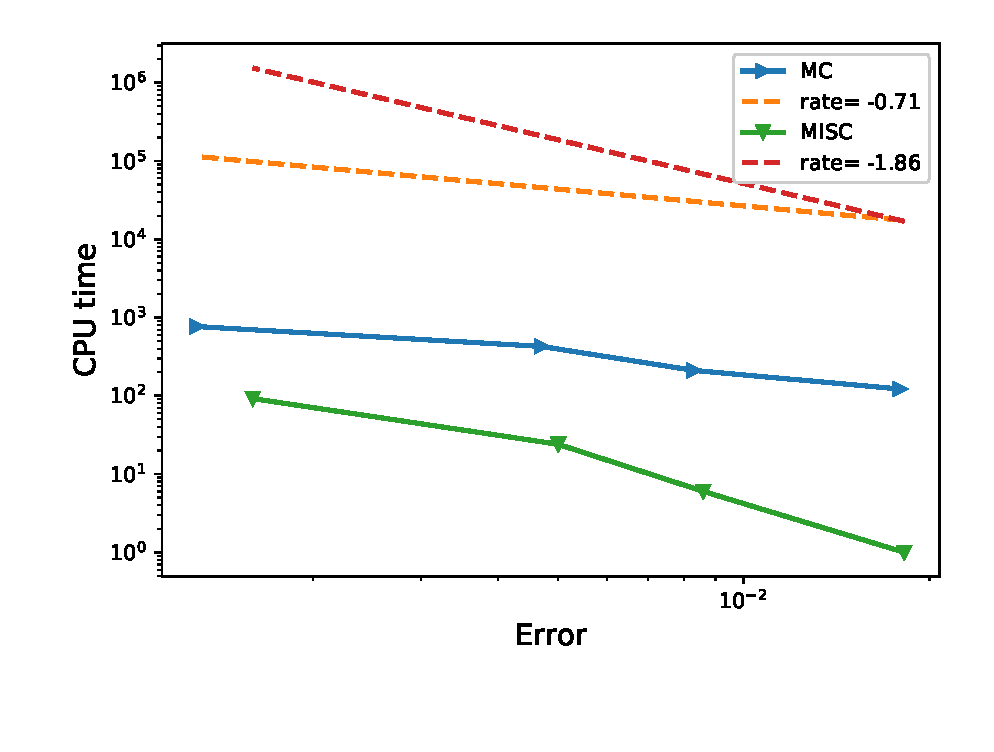
\includegraphics[width=0.5\linewidth]{./figures/rBergomi_Complexity_rates/set5/error_vs_time_set5}

	\caption{Complexity plot for   MC and MISC for case set $3$ parameters of table \ref{table:Reference solution, using MC with $500$ time steps, of Call option price under rBergomi model, for different parameter constellation.}.}
	\label{fig:Complexity plot for MC and MISC for Case set $3$ parameters}
\end{figure}



\FloatBarrier
\subsubsection*{With Richardson extrapolation (level $1$)}
\begin{table}[h!]
	\centering
	\begin{tabular}{l*{6}{c}r}
		Method \textbackslash  Steps    &$1-2$         & $2-4$ & $4-8$ & $8-16$\\
		\hline
%		MISC ($TOL_{\text{MISC}}=5.10^{-1}$)   &$ 0.1261$ & $0.1220$ & $0.1222$ & $0.1223$\\
		MISC ($TOL_{\text{MISC}}=10^{-1}$)   &$ 0.1261$ & $0.1220$  &$0.1222$ & $0.1226$\\
%		MISC ($TOL_{\text{MISC}}=5.10^{-2}$)   &$ 0.1261$ & $0.1220$  & $0.1222$ & $0.1240$ \\
		MISC ($TOL_{\text{MISC}}=10^{-2}$)   &$ 0.1267$ & $0.1230$ & $0.1245$ & $0.1247$  \\	
		MISC ($TOL_{\text{MISC}}=10^{-3}$)   &$0.1285$ & $0.1247$ & $0.1247$ &  $0.1247$ \\
		MISC ($TOL_{\text{MISC}}=10^{-4}$)  &$0.1285$ & $0.1247$ & $0.1247$ & $-$ \\
			MISC ($TOL_{\text{MISC}}=10^{-5}$)  &$0.1285$ & $0.1247$ &  $0.1247$ & $-$ \\
	
		\hline
		MC method ($M=10^{7}$)   & $     0.1284$  & $ 
		0.1251$  & $0.1249$ & $  0.1248$ \\		
		\hline
	\end{tabular}
	\caption{Call option price of the different methods for different number of time steps. Case set $3$ parameters of table \ref{table:Reference solution, using MC with $500$ time steps, of Call option price under rBergomi model, for different parameter constellation.}, using Richardson extrapolation (level $1$).}
	\label{table:  Call option price of the different methods for different number of time steps. Case set $5$ parameter, using Richardson extrapolation (level $3$)}
\end{table}



\begin{table}[h!]
	\centering
	\begin{tabular}{l*{6}{c}r}
		Method \textbackslash  Steps            & $1-2$ & $2-4$ & $4-8$ & $8-16$  \\
		\hline
		MC Bias ($M=10^7$)  &$\underset{(  0.0037
			)}{\mathbf{0.0295}}$  & $\underset{( 0.0003)}{\mathbf{0.0025}}$  & $\underset{(   0.0001)}{\mathbf{0.0009}}$  & $\underset{(  6.2e-05)}{\mathbf{0.0005}}$ \\	
		
		MC Statistical error ($M=10^7$)   & $\underset{(  4.4e-05)}{\mathbf{3.5e-04}}$  & $\underset{(   4.2e-05)}{\mathbf{3.4e-04}}$  & $\underset{(  4.1e-05)}{\mathbf{3.3e-04}}$ & $\underset{(  4.1e-05)}{\mathbf{3.3e-04}}$ \\	
	
		\hline
	\end{tabular}
	\caption{Bias and statistical errors of MC   for computing call option price  for different number of time steps. Case set $3$ parameters in tabel \ref{table:Reference solution, using MC with $500$ time steps, of Call option price under rBergomi model, for different parameter constellation.}, with Richardson extrapolation (level $1$). The numbers between parentheses are the corresponding absolute errors.}
	\label{Bias and Statistical errors of MC ($M=10^7$)  for computing Call option price  for different number of time steps. Case set $3$ parameters, with Richardson extrapolation (level1). The numbers between parentheses are the corresponding absolute errors.}
\end{table}








\begin{figure}[h!]
	\centering
	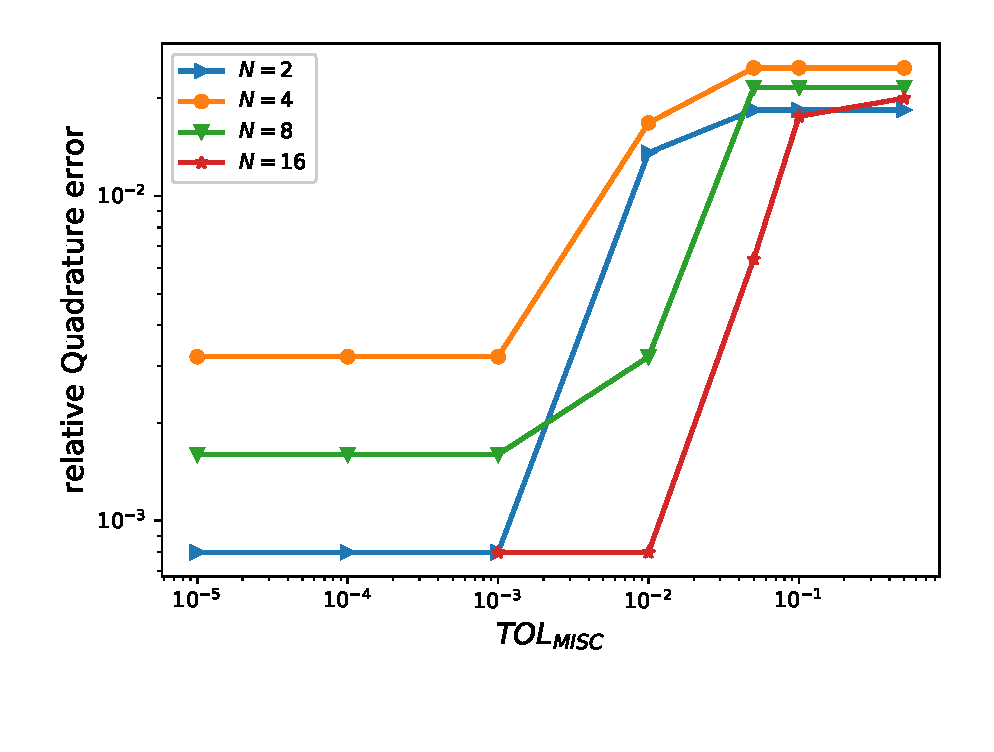
\includegraphics[width=0.5\linewidth]{./figures/rBergomi_MISC_quadratre_error/vs_TOL/set5/relative_quad_error_wrt_MISC_TOL_set5_with_rich}
	
	
	\caption{Quadrature error of MISC, with  different tolerances,  to compute call option price, for different number of time steps. Case  set $3$ parameters, with Richardson extrapolation.  See detailed values  in table \ref{Quadrature error of MISC to compute Call option price of the different tolerances for different number of time steps. Case set $3$ parameters, with Richardson extrapolation(level $1$). The numbers between parentheses are the corresponding absolute errors.}.}
	\label{fig:Quadrature_error_set3_rich}
\end{figure}

\begin{table}[h!]
	\centering
	\begin{tabular}{l*{6}{c}r}
		Method \textbackslash  Steps           & $2-4$ & $4-8$ & $8-16$  \\
		\hline
%		MISC ($TOL_{\text{MISC}}=5.10^{-1}$)  & $0.0273$  & $0.0225$ & $0.0205$  \\
		MISC ($TOL_{\text{MISC}}=10^{-1}$)  &$0.0273$  &$0.0225$ & $0.0181$  \\
%		MISC ($TOL_{\text{MISC}}=5.10^{-2}$)  & $0.0273$  &$0.0225$ & $0.0069$  \\
			MISC ($TOL_{\text{MISC}}=10^{-2}$)  & $0.0193$  & $0.0041$ & $\red{0.0013}$  \\
		MISC ($TOL_{\text{MISC}}=10^{-3}$)  & $\red{0.0057}$  & $\red{0.0025}$ & $0.0013$  \\
		MISC ($TOL_{\text{MISC}}=10^{-4}$)    &$0.0057$  & $0.0033$  & $-$  \\
			MISC ($TOL_{\text{MISC}}=10^{-5}$)    &$0.0057$   &  $0.0033$ & $-$  \\	
	\hline

		MC    & $\red{\mathbf{0.0073}}$  &   $\red{\mathbf{0.0025}}$  &  $\red{\mathbf{0.0013}}$  \\
		\hline
	\end{tabular}
	\caption{Total relative error of MISC, with different tolerances, and MC to compute Call option price  for different number of time steps. Case set $3$ parameters in table \ref{table:Reference solution, using MC with $500$ time steps, of Call option price under rBergomi model, for different parameter constellation.}, with Richardson extrapolation(level $1$). The numbers between parentheses are the corresponding absolute errors. The values marked in red, for MISC method, correspond to the total relative errors associated with  stable quadrature errors for MISC, and will be used for complexity comparison against MC.}
	\label{Total  error of MISC and MC to compute Call option price of the different tolerances for different number of time steps. Case set $3$ parameters, with Richardson extrapolation(level $1$). The numbers between parentheses are the corresponding absolute errors.}
\end{table}



\begin{table}[h!]
	\centering
	\begin{tabular}{l*{6}{c}r}
		Method \textbackslash  Steps            & $2-4$ & $4-8$ & $8-16$ &   \\
		\hline
%		MISC ($TOL_{\text{MISC}}=5.10^{-1}$)    & $0.15$ & $0.25$ & $0.5$  \\
		MISC ($TOL_{\text{MISC}}=10^{-1}$)   & $0.15$ & $0.25$ & $1$  \\
%		MISC ($TOL_{\text{MISC}}=5.10^{-2}$)    &  $0.15$ & $0.25$ & $12.5$  \\
		MISC ($TOL_{\text{MISC}}=10^{-2}$)   & $0.6$ & $10$ & $\red{112}$  \\
		MISC ($TOL_{\text{MISC}}=10^{-3}$)  & $\red{3.5}$ & $\red{34}$ & $3150$ \\
		MISC ($TOL_{\text{MISC}}=10^{-4}$) & $11$ & $328$ & $-$  \\
		MISC ($TOL_{\text{MISC}}=10^{-5}$)   & $39$ & $2160$ & $-$  \\
		\hline	
			MC  & $\red{45}$  & $\red{438}$  & $\red{2240}$ \\
			
			\hline
				Ratio of $\left(\text{MC}/ \text{MISC} \right)$   & $\red{13}$  & $\red{13}$  & $\red{20}$ \\

		\hline
	\end{tabular}
	\caption{Comparison of the computational time (in Seconds) of  MC and MISC, using Richardson extrapolation (level $1$), used to compute Call option price of rBergomi model for different number of time steps. Case set $3$ parameters in table \ref{table:Reference solution, using MC with $500$ time steps, of Call option price under rBergomi model, for different parameter constellation.}. The
average MC CPU time is computed over 10 runs.}
	\label{Comparsion of the computational time of  MC and MISC, using Richardson extrapolation (level $1$), used to compute Call option price of rBergomi model for different number of time steps. Case set $3$ parameters}
\end{table}




	\begin{figure}[h!]
	\centering
	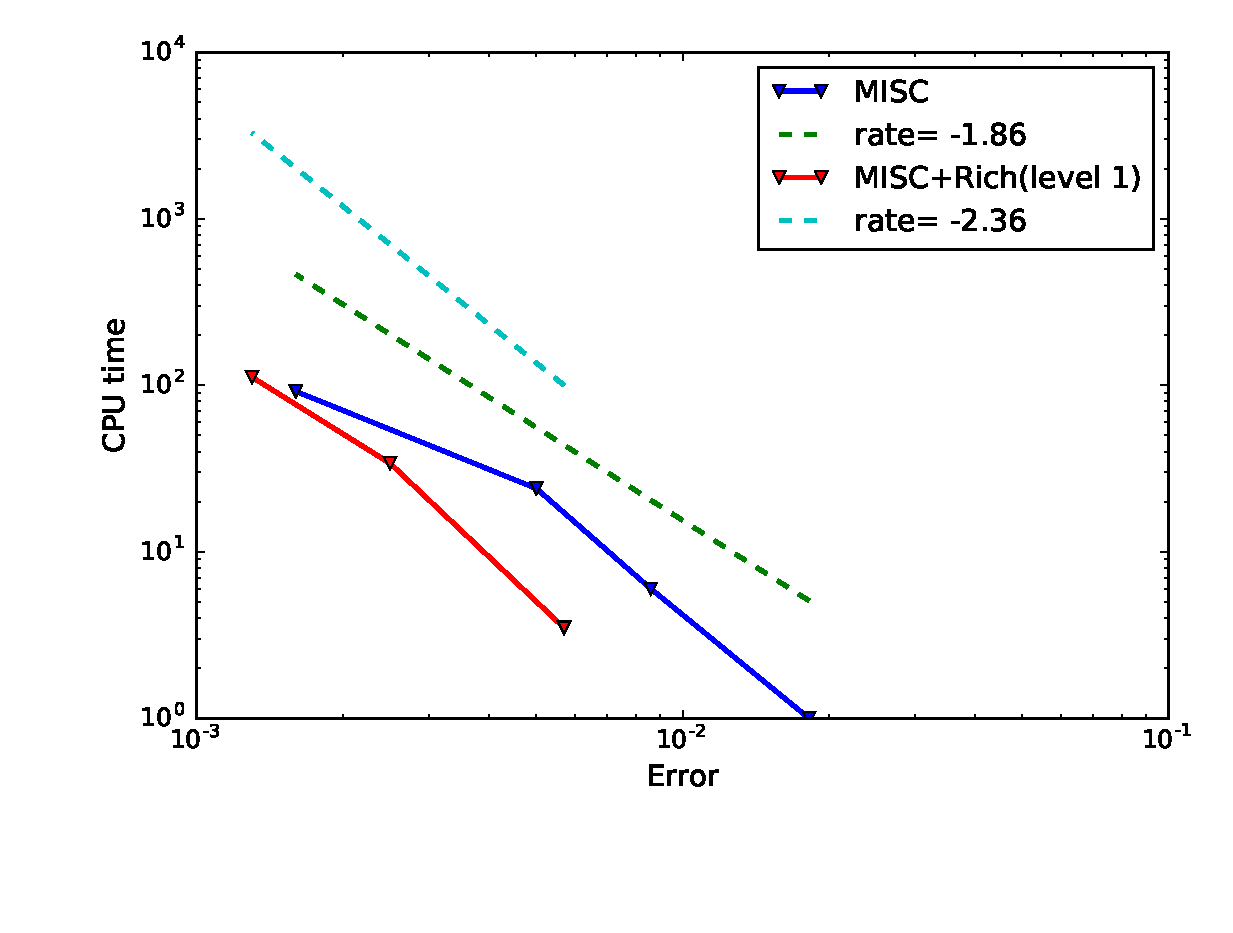
\includegraphics[width=0.5\linewidth]{./figures/rBergomi_Complexity_rates/set5/error_vs_time_set5_comparison}
	
	\caption{Complexity plot for  MISC (with/without) Richardson extrapolation for case set $3$ parameters of table \ref{table:Reference solution, using MC with $500$ time steps, of Call option price under rBergomi model, for different parameter constellation.}.}
	\label{fig:Complexity plot for  MISC for case set $3$ parameters, comparison}
\end{figure}







\FloatBarrier
\subsubsection{Case of set $4$ parameters in table \ref{table:Reference solution, using MC with $500$ time steps, of Call option price under rBergomi model, for different parameter constellation.}}\label{sec:Case of set 4 parameters}

\begin{table}[h!]
	\centering
	\begin{tabular}{l*{6}{c}r}
		Method \textbackslash  Steps            & $2$ & $4$ & $8$ & $16$ &   \\
		\hline
%		MISC ($TOL_{\text{MISC}}=5.10^{-1}$)  & $0.2413$ & $0.2403$ & $0.2403$ & $0.2396$  \\
		MISC ($TOL_{\text{MISC}}=10^{-1}$)  & $0.2413$ &$0.2403$& $0.2403$ & $0.2397$   \\
%		MISC ($TOL_{\text{MISC}}=5.10^{-2}$)  &$0.2413$ & $0.2403$ & $0.2403$ & $0.2406$  \\
		MISC ($TOL_{\text{MISC}}=10^{-2}$)  &$0.2413$ & $0.2403$ & $0.2409$ & $0.2413$  \\
		
		MISC ($TOL_{\text{MISC}}=10^{-3}$)  & $0.2413$ & $0.2411$ & $0.2414$ & $0.2413$  \\
		MISC ($TOL_{\text{MISC}}=10^{-4}$)  &  $0.2421$ & $0.2416$ & $0.2414$ & $-$  \\
		
		MISC ($TOL_{\text{MISC}}=10^{-5}$)  & $0.2421$ &$0.2416$ &  $0.2414$ & $-$  \\
		\hline
		MC method ($M=5.10^{6}$)   & $0.2420$ & $0.2416$  & $0.2414$ & $0.2413$ \\		
		
		\hline
	\end{tabular}
	\caption{ Call option price of the different methods for different number of time steps. Case set $4$ parameters in table \ref{table:Reference solution, using MC with $500$ time steps, of Call option price under rBergomi model, for different parameter constellation.}, without Richardson extrapolation.}
	\label{table: Call option price of the different methods for different number of time steps. Case set 4}
\end{table}


\begin{table}[h!]
	\centering
	\begin{tabular}{l*{6}{c}r}
		Method \textbackslash  Steps            & $2$ & $4$ & $8$ & $16$  \\
		\hline
		MC Bias ($M=5.10^6$)   & 	$ \underset{(    0.0013)}{\mathbf{0.0054}}$  & $\underset{(0.0008)}{\mathbf{0.0035
		}}$  & $\underset{(0.0007)}{\mathbf{0.0029}}$ & $\underset{(0.0006)}{\mathbf{0.0024}}$\\ 
		
		MC Statistical error ($M=5.10^6$)  &  $\underset{(   8.3e-05)} {\mathbf{3.4e-04}}$  & $\underset{(8.1e-05)} {\mathbf{3.4e-04}}$  & $\underset{(8.0e-05)} {\mathbf{3.3e-04 }}$ & $\underset{(8.0e-05)} {\mathbf{3.3e-04}}$	\\
		
		\hline
	\end{tabular}
	\caption{Bias and statistical errors of MC   for computing call option price  for different number of time steps. Case set $4$, without Richardson extrapolation. The numbers between parentheses are the corresponding absolute errors.}
	\label{Bias and Statistical errors of MC ($M=5.10^6$)  for computing Call option price  for different number of time steps. Case set 4, without Richardson extrapolation. The numbers between parentheses are the corresponding absolute errors.}
\end{table}





\begin{figure}[h!]
	\centering
	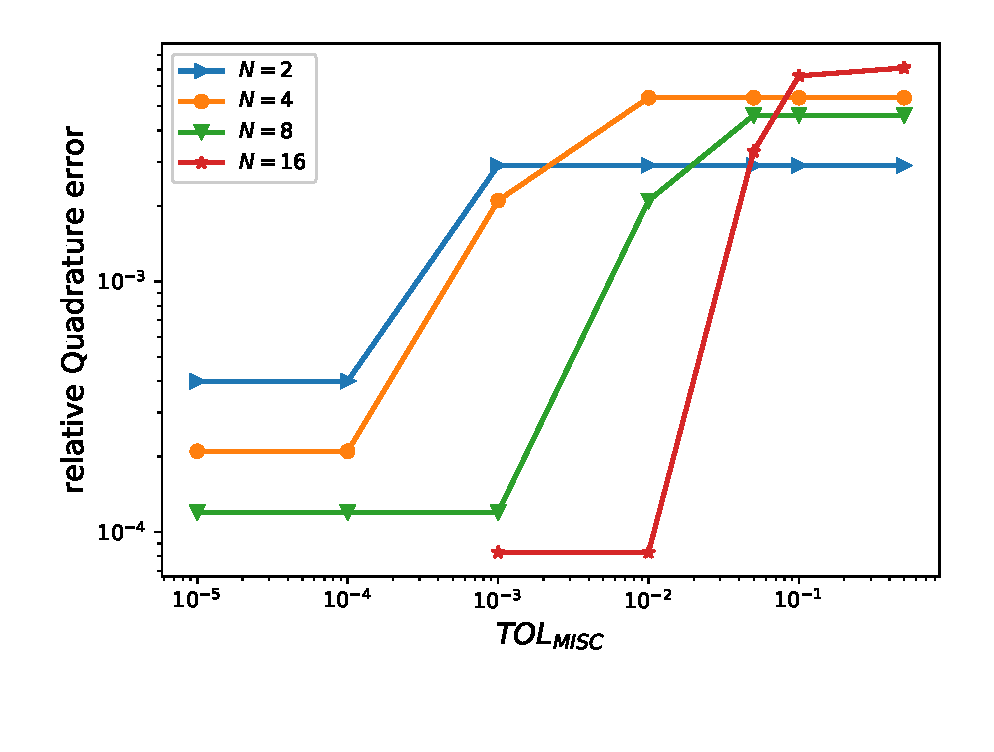
\includegraphics[width=0.5\linewidth]{./figures/rBergomi_MISC_quadratre_error/vs_TOL/set6/relative_quad_error_wrt_MISC_TOL_set6_non_rich}
	
	
	\caption{Quadrature error of MISC, with different tolerances, to compute call option price  for different number of time steps. Case  set $4$ parameters, without Richardson extrapolation.  See detailed values  in table \ref{Quadrature error of MISC to compute Call option price of the different tolerances for different number of time steps. Case  set $4$ parameters, without Richardson extrapolation. The numbers between parentheses are the corresponding absolute errors.}}
	\label{fig:Quadrature_error_set4}
\end{figure}





\begin{table}[h!]
	\centering
	\begin{tabular}{l*{6}{c}r}
		Method \textbackslash  Steps            & $2$ & $4$ & $8$ & $16$  \\
		\hline
%		MISC ($TOL_{\text{MISC}}=5.10^{-1}$)  & $\mathbf{0.0083}$ & $\mathbf{0.0089}$ & $\mathbf{ 0.0075}$ & $\mathbf{ 0.0095}$  \\
		MISC ($TOL_{\text{MISC}}=10^{-1}$)  &  $\mathbf{0.0083}$ & $\mathbf{0.0089}$& $\mathbf{ 0.0075}$ & $\mathbf{ 0.0090}$   \\
%		MISC ($TOL_{\text{MISC}}=5.10^{-2}$)  & $\mathbf{0.0083}$ & $\mathbf{0.0089}$ & $\mathbf{ 0.0075}$ & $\mathbf{ 0.0057}$  \\
		MISC ($TOL_{\text{MISC}}=10^{-2}$)  &  $\mathbf{0.0083}$ & $\mathbf{0.0089}$& $\mathbf{ 0.0050}$ & $\mathbf{ \red{0.0025}}$  \\
		MISC ($TOL_{\text{MISC}}=10^{-3}$)  &  $\mathbf{0.0083}$& $\mathbf{0.0056}$& $\mathbf{\red{0.0030}}$  & $\mathbf{ 0.0025}$  \\
		MISC ($TOL_{\text{MISC}}=10^{-4}$)  &  $\mathbf{\red{0.0058}}$ & $\mathbf{\red{0.0037}}$& $\mathbf{0.0030}$ & $\mathbf{ -}$ \\
		MISC ($TOL_{\text{MISC}}=10^{-5}$)  &  $\mathbf{0.0058}$ & $\mathbf{0.0037}$& $\mathbf{0.0030}$ & $\mathbf{ -}$ 
		\\
		\hline
		MC    & $\mathbf{\red{0.0057}}$  & $\mathbf{ \red{0.0038}}$  & $\mathbf{\red{0.0032}}$ & $\mathbf{ \red{0.0027}}$  \\		
		\hline
	\end{tabular}
	\caption{Total relative error of MISC,different tolerances, and MC to compute call option price  for different number of time steps. Case set $4$ parametrs of table \ref{table:Reference solution, using MC with $500$ time steps, of Call option price under rBergomi model, for different parameter constellation.}, without Richardson extrapolation. The numbers between parentheses are the corresponding absolute errors. The values marked in red, for MISC method, correspond to the total relative errors associated with  stable quadrature errors for MISC, and will be used for complexity comparison against MC.}
	\label{Total error of MISC and MC to compute Call option price of the different tolerances for different number of time steps. Case set 4, without Richardson extrapolation. The numbers between parentheses are the corresponding absolute errors.}
\end{table}


\begin{table}[h!]
	\centering
	\begin{tabular}{l*{6}{c}r}
		Method \textbackslash  Steps            & $2$ & $4$ & $8$ & $16$ &   \\
		\hline
%		MISC ($TOL_{\text{MISC}}=5.10^{-1}$)  & $0.1$ & $0.1$ & $0.1$ & $0.3$  \\
		MISC ($TOL_{\text{MISC}}=10^{-1}$)  & $0.1$ & $0.1$ & $0.1$ & $1$ \\
%		MISC ($TOL_{\text{MISC}}=5.10^{-2}$)  & $0.1$ & $0.1$ & $0.1$ & $22$  \\
		MISC ($TOL_{\text{MISC}}=10^{-2}$)  & $0.1$ & $0.15$ & $9$ & $\red{112}$ \\
		MISC ($TOL_{\text{MISC}}=10^{-3}$)  & $0.2$ & $2$ & $\red{27}$ & $2226$ \\
		MISC ($TOL_{\text{MISC}}=10^{-4}$)  & $\red{1}$ & $\red{6}$ & $136$ & $-$\\
		MISC ($TOL_{\text{MISC}}=10^{-5}$)  & $2$ & $18$ & $1559$ & $-$
		\\
		\hline
		MC method   & $ \red{141}
		
		$  & $  \red{246}$  & $  \red{461}$ & $ \red{820}
		$  \\	
		\hline
		Ratio of $\left(MC/MISC \right)$ & $ \red{141}
		
		$  & $  \red{
			41
		}$  & $  \red{    17
		}$ & $ \red{ 7}
		$  \\	
%		
		\hline
	\end{tabular}
	\caption{Comparison of the computational time (in Seconds) of  MC and MISC, used to compute call option price of rBergomi model for different number of time steps. Case set $4$ parameters of table \ref{table:Reference solution, using MC with $500$ time steps, of Call option price under rBergomi model, for different parameter constellation.}. The average  MC CPU time is computed over $10$ runs. }
	\label{Comparsion of the computational time of  MC and MISC, used to compute Call option price of rBergomi model for different number of time steps. Case set4}
\end{table}




	\begin{figure}[h!]
	\centering
	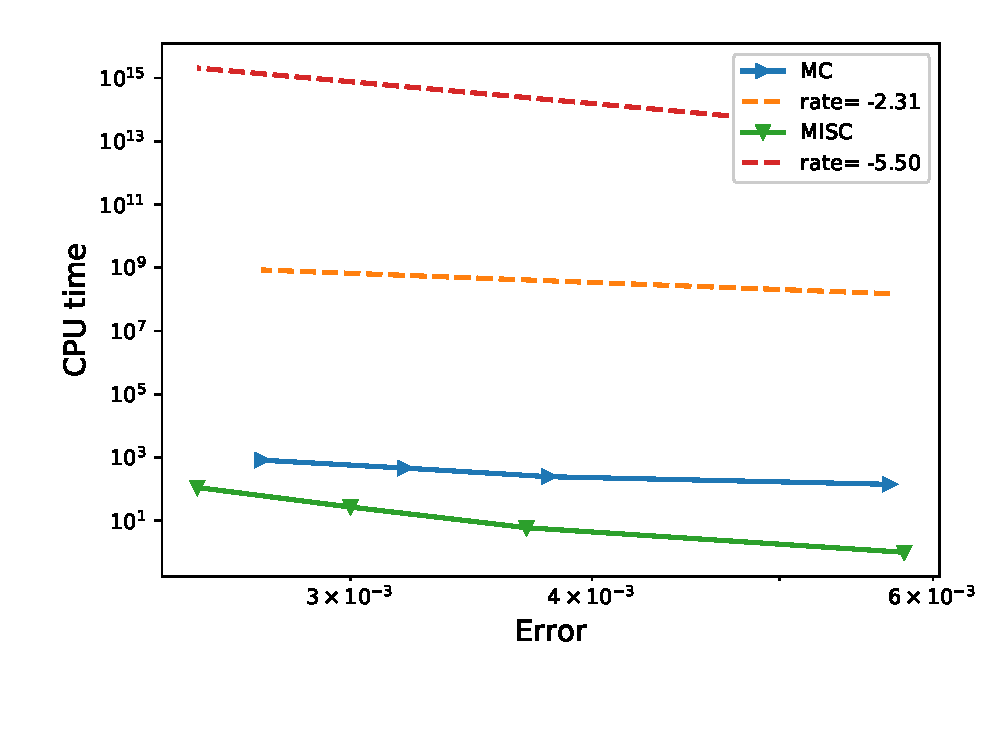
\includegraphics[width=0.5\linewidth]{./figures/rBergomi_Complexity_rates/set6/error_vs_time_set6}
	
	\caption{Complexity plot for   MC and MISC for case set $4$ parameters of table \ref{table:Reference solution, using MC with $500$ time steps, of Call option price under rBergomi model, for different parameter constellation.}.}
	\label{fig:Complexity plot for MC and MISC for case set $4$ parameters}
\end{figure}
\FloatBarrier
\subsubsection{Case of set $5$ parameters in table \ref{table:Reference solution, using MC with $500$ time steps, of Call option price under rBergomi model, for different parameter constellation.}}\label{sec:Case of set 5 parameters}

\begin{table}[h!]
	\centering
	\begin{tabular}{l*{6}{c}r}
		Method \textbackslash  Steps            & $2$ & $4$ & $8$ & $16$ &   \\
		\hline
%		MISC ($TOL_{\text{MISC}}=5.10^{-1}$)  & $0.0590$ & $0.0564$ & $0.0552$ & $0.0546$  \\
		MISC ($TOL_{\text{MISC}}=10^{-1}$)  & $0.0590$ &$0.0564$& $0.0552$ & $0.0546$   \\
%		MISC ($TOL_{\text{MISC}}=5.10^{-2}$)  &$0.0590$ & $0.0564$ & $0.0552$ & $0.0557$  \\
		MISC ($TOL_{\text{MISC}}=10^{-2}$)  &$0.0590$ &$0.0564$ & $0.0574$ & $0.0572$  \\
		
		MISC ($TOL_{\text{MISC}}=10^{-3}$)  & $0.0605$ & $0.0587$ & $0.0579$ & $0.0575$  \\
		MISC ($TOL_{\text{MISC}}=10^{-4}$)  &  $0.0605$ & $0.0587$ & $0.0576$ & $-$  \\
		
		MISC ($TOL_{\text{MISC}}=10^{-5}$)  & $0.0605$ & $0.0587$ &  $0.0579$ & $-$  \\
		\hline
		MC method ($M=5.10^{6}$)   & $0.0605$ & $0.0587$  & $0.0579$ & $0.0576$ \\		
		
		\hline
	\end{tabular}
	\caption{ Call option price of the different methods for different number of time steps. Case of set $5$ parameters in table \ref{table:Reference solution, using MC with $500$ time steps, of Call option price under rBergomi model, for different parameter constellation.}, without Richardson extrapolation.}
	\label{table: Call option price of the different methods for different number of time steps. Case set 5}
\end{table}


\begin{table}[h!]
	\centering
	\begin{tabular}{l*{6}{c}r}
		Method \textbackslash  Steps            & $2$ & $4$ & $8$ & $16$  \\
		\hline
		MC Bias ($M=5.10^6$)   & 	$ \underset{(0.0037
			)}{\mathbf{0.0650}}$  & $\underset{(0.0019)}{\mathbf{0.0330
		}}$  & $\underset{(0.0012)}{\mathbf{0.0202}}$ & $\underset{(0.0007)}{\mathbf{0.0130}}$\\ 
		
		MC Statistical error ($M=5.10^6$)  &  $\underset{(   4.0e-05)} {\mathbf{7.0e-04}}$  & $\underset{(3.8e-05)} {\mathbf{6.7e-04}}$  & $\underset{(3.7e-05)} {\mathbf{6.5e-04 }}$ & $\underset{(3.6e-05)} {\mathbf{6.3e-04}}$	\\
		
		\hline
	\end{tabular}
	\caption{Bias and statistical errors of MC   for computing call option price  for different number of time steps. Case set $5$, without Richardson extrapolation. The numbers between parentheses are the corresponding absolute errors.}
	\label{Bias and Statistical errors of MC ($M=5.10^6$)  for computing Call option price  for different number of time steps. Case set 5, without Richardson extrapolation. The numbers between parentheses are the corresponding absolute errors.}
\end{table}
%
%
%








\begin{figure}[h!]
	\centering
	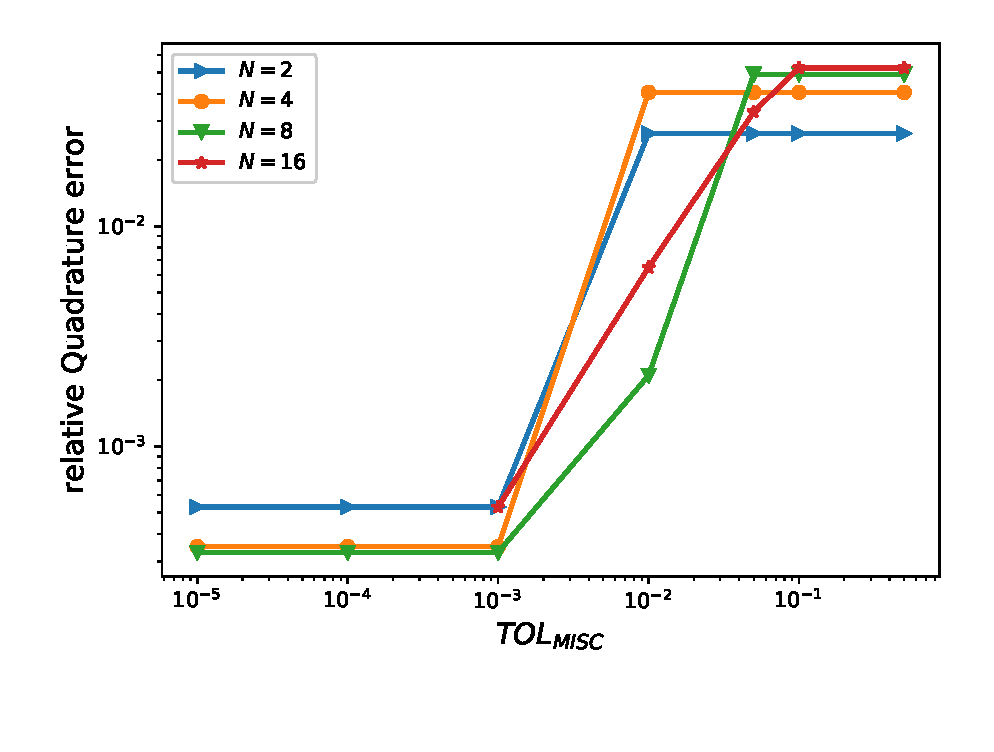
\includegraphics[width=0.5\linewidth]{./figures/rBergomi_MISC_quadratre_error/vs_TOL/set7/relative_quad_error_wrt_MISC_TOL_set7_non_rich}
	
	
	\caption{Quadrature error of MISC, with  different tolerances,  to compute call option price  for different number of time steps. Case  set $5$ parameters, without Richardson extrapolation.  See detailed values  in table \ref{Quadrature error of MISC to compute Call option price of the different tolerances for different number of time steps. Case  set $5$ parameters, without Richardson extrapolation. The numbers between parentheses are the corresponding absolute errors.}}
	\label{fig:Quadrature_error_set5}
\end{figure}


%
%
%
\begin{table}[h!]
	\centering
	\begin{tabular}{l*{6}{c}r}
		Method \textbackslash  Steps            & $2$ & $4$ & $8$ & $16$  \\
		\hline
%		MISC ($TOL_{\text{MISC}}=5.10^{-1}$)  & $\mathbf{0.0914}$ & $\mathbf{0.0736}$ & $\mathbf{ 0.0693}$ & $\mathbf{ 0.0654}$  \\
		MISC ($TOL_{\text{MISC}}=10^{-1}$)  & $\mathbf{0.0914}$ & $\mathbf{0.0736}$& $\mathbf{ 0.0693}$ & $\mathbf{ 0.0654}$   \\
%		MISC ($TOL_{\text{MISC}}=5.10^{-2}$)  & $\mathbf{0.0914}$ & $\mathbf{0.0736}$ & $\mathbf{ 0.0693}$ & $\mathbf{ 0.0461}$  \\
		MISC ($TOL_{\text{MISC}}=10^{-2}$)  &  $\mathbf{0.0914}$& $\mathbf{0.0736}$& $\mathbf{ 0.0223}$ & $\mathbf{ 0.0195}$  \\
		MISC ($TOL_{\text{MISC}}=10^{-3}$)  &  $\mathbf{\red{0.0655}}$& $\mathbf{\red{0.0334}}$& $\mathbf{\red{0.0205}}$  & $\mathbf{ \red{0.0135}}$  \\
		MISC ($TOL_{\text{MISC}}=10^{-4}$)  &  $\mathbf{0.0655}$& $\mathbf{0.0334}$& $\mathbf{0.0205}$ & $\mathbf{ -}$ \\
		MISC ($TOL_{\text{MISC}}=10^{-5}$)  &  $\mathbf{0.0655}$ & $\mathbf{0.0334}$& $\mathbf{0.0205}$ & $\mathbf{ -}$ 
		\\
		\hline
		MC    & $\mathbf{\red{0.0657}}$  & $\mathbf{ \red{0.0337}}$  & $\mathbf{\red{0.0209}}$ & $\mathbf{ \red{0.0136}}$  \\		
		\hline
	\end{tabular}
	\caption{Total relative error of MISC, with  different tolerances,  and MC to compute call option price  for different number of time steps. Case  set $5$ parametrs of table \ref{table:Reference solution, using MC with $500$ time steps, of Call option price under rBergomi model, for different parameter constellation.}, without Richardson extrapolation. The numbers between parentheses are the corresponding absolute errors. The values marked in red, for MISC method, correspond to the total relative errors associated with  stable quadrature errors for MISC, and will be used for complexity comparison against MC.}
	\label{Total error of MISC and MC to compute Call option price of the different tolerances for different number of time steps. Case set 5, without Richardson extrapolation. The numbers between parentheses are the corresponding absolute errors.}
\end{table}


\begin{table}[h!]
	\centering
	\begin{tabular}{l*{6}{c}r}
		Method \textbackslash  Steps            & $2$ & $4$ & $8$ & $16$ &   \\
		\hline
%		MISC ($TOL_{\text{MISC}}=5.10^{-1}$)  & $0.1$ & $0.1$ & $0.2$ & $0.5$  \\
		MISC ($TOL_{\text{MISC}}=10^{-1}$)  & $0.1$ & $0.1$ & $0.2$ & $0.5$ \\
%		MISC ($TOL_{\text{MISC}}=5.10^{-2}$)  & $0.1$ & $0.1$ & $0.2$ & $5$  \\
		MISC ($TOL_{\text{MISC}}=10^{-2}$)  & $0.1$ & $0.1$ & $8$ & $97$ \\
		MISC ($TOL_{\text{MISC}}=10^{-3}$)  & $\red{0.7}$ & $\red{4}$ & $\red{26}$ & $\red{1984}$ \\
		MISC ($TOL_{\text{MISC}}=10^{-4}$)  & $1$ & $8$ & $173$ & $-$\\
		MISC ($TOL_{\text{MISC}}=10^{-5}$)  & $1$ & $32$ & $2129$ & $-$
		\\
		\hline
		MC method   & $ \red{154}
		
		$  & $  \red{229}$  & $  \red{420}$ & $ \red{938}
		$  \\	
		\hline
		Ratio of $\left(MC/MISC \right)$ & $ \red{   220}
		
		$  & $  \red{
		 57
		}$  & $  \red{    16
		}$ & $ \red{ 0.5}
		$  \\	
				
		\hline
	\end{tabular}
	\caption{Comparison of the computational time (In seconds) of  MC and MISC, used to compute Call option price of rBergomi model for different number of time steps. Case set $5$ parametrs of table \ref{table:Reference solution, using MC with $500$ time steps, of Call option price under rBergomi model, for different parameter constellation.}. The average  MC CPU time is computed over $10$ runs. }
	\label{Comparsion of the computational time of  MC and MISC, used to compute Call option price of rBergomi model for different number of time steps. Case set5}
\end{table}
	\begin{figure}[h!]
	\centering
	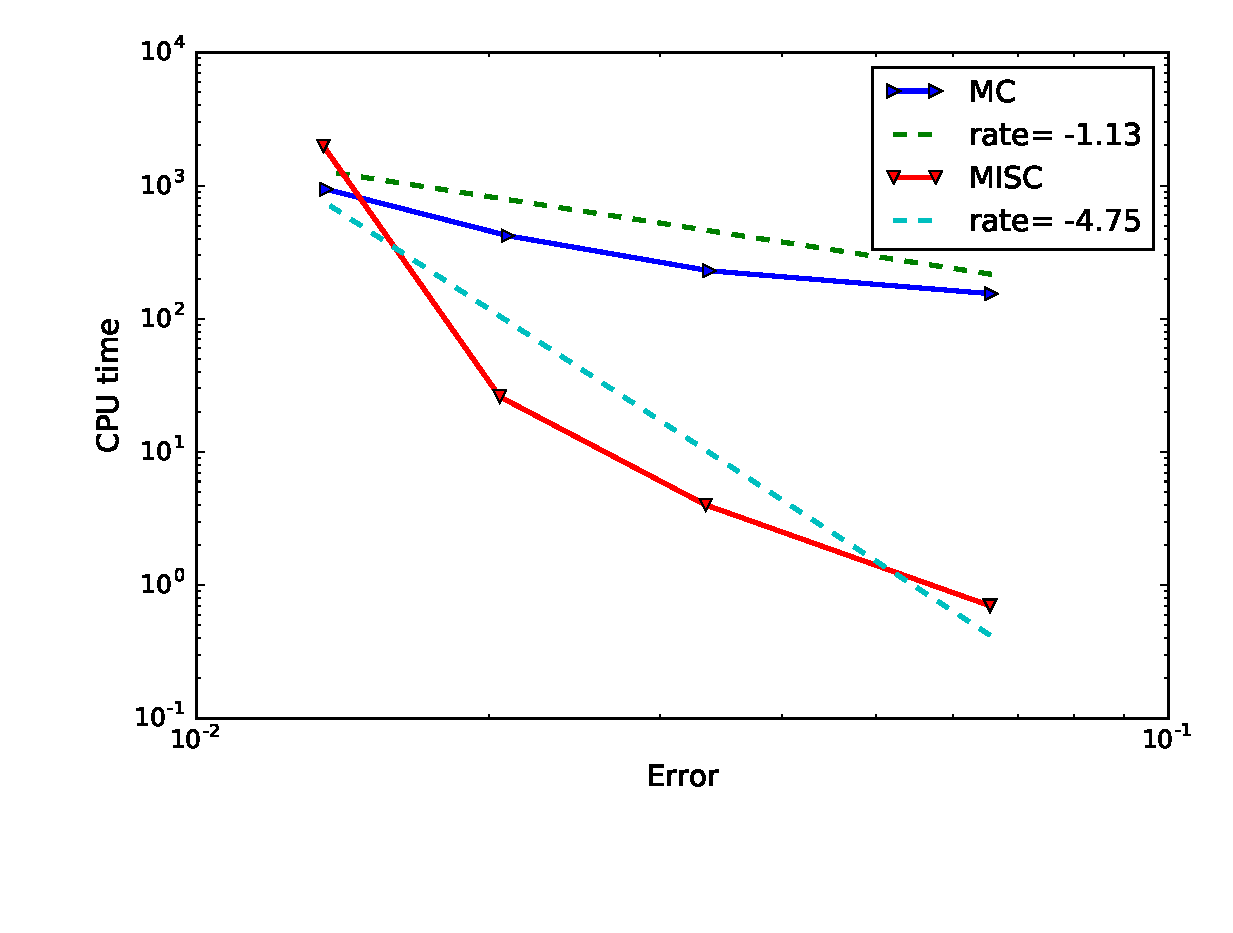
\includegraphics[width=0.5\linewidth]{./figures/rBergomi_Complexity_rates/set7/error_vs_time_set7}
	
	\caption{Complexity plot for   MC and MISC for case set $5$ parameters of table \ref{table:Reference solution, using MC with $500$ time steps, of Call option price under rBergomi model, for different parameter constellation.}.}
	\label{fig:Complexity plot for MC and MISC for Case set $5$ parameters}
\end{figure}
\FloatBarrier







\section{Conclusions and future work}

In this work,  we propose a novel hierarchical fast option pricer,  based on a  hierarchical adaptive sparse grids quadrature, specifically  multi-index stochastic collocation (MISC) as in  \cite{haji2016multi}, coupled with Brownian bridge construction and Richardson extrapolation, for options whose underlyings  follow rBergomi model as in \cite{bayer2016pricing}.  In order to use a  variant of adaptive sparse grids quadrature for our purposes, we had to solve two main issues, that constitutes the two stages of our new designed method. In the first stage, we smoothen the integrand by using the conditional expectation trick as was proposed by \cite{romano1997contingent}, in the context of Markovian stochastic volatility  models.   In a second stage, we applied a variant of hierarchical adaptive sparse grids quadrature, specifically MISC as in \cite{haji2016multi}, to solve the integration problem. In this stage, we had to apply two pre-transformations before using the MISC solver, in order to overcome the issue of facing a high dimensional integrand, due to the discretization scheme used for simulating the rBergomi dynamics. Given that MISC profits from anisotropy, the first pre-transformation consists of applying a hierarchical  path generation method, based on Brownian
bridge (BB) construction, with the aim of reducing the effective dimension. The second pre-transformation consists of applying Richardson extrapolation to reduce the bias, resulting in reducing the needed number of time steps in the coarsest level to achieve a certain error tolerance, and therefore,  the maximum number of dimensions needed for the integration problem.

Given that the only prevalent option, in this context, is to use different variants of MC method, our first contribution  is that we design an alternative approach based on  adaptive sparse grid quadrature, which opens a new persepective for experts in this field to investigate the performance of other methods besides MC, to solve pricing and calibration problems related to rBergomi model. Our second contribution is that  we reduce the computational cost not only through variance reduction, as in  \cite{mccrickerd2017turbocharging}, by using the conditional expectation, but also through bias reduction through using Richardson extrapolation, which contibutes also to reducing the dimension of the integration problem associated to computing the option price. Finally, assuming one targets prices estimates with a suffciently small degree of error tolerance, our thrid contribution is manifested by the observed substantial computational gains  over standard MC method, when pricing under rBergomi model. We show  these gains through our numerical experiments for  different parameters constellations. 

In this paper, we limit ourselves to compare our novel proposed method against standard MC. A more systematic comparison against the variant of MC proposed in \cite{mccrickerd2017turbocharging}  can be carried over but this is left for a future work. Another  eventual direction of research may also investigate the performance of QMC for such problems. Finally, accelerating  our novel designed method can be reached  by coupling MISC with a more optimal hierarchical path generation method than Brownian bridge construction, such as PCA or LT transformations, etc \dots

\

\textbf{Acknowledgments} C. Bayer gratefully acknowledges support from the German Research Foundation (DFG, grant BA5484/1). This work was supported by the KAUST Office of Sponsored Research (OSR) under Award No. URF/1/2584-01-01 and the Alexander von Humboldt Foundation. C. Ben Hammouda and R. Tempone are members of the KAUST SRI Center for Uncertainty Quantification in Computational Science and Engineering. The authors would like to thank Eric Joseph Hall and Erik von Schwerin for their helpful and constructive comments that greatly contributed to improving the final version of the paper. 



 %%%%%%%%%%%%%%%%%%%%%%%%%%%%%%%%%%%%%%%%%%
%References
%%%%%%%%%%%%%%%%%%%%%%%%%%%%%%%%%%%%%%%%%%

\bibliographystyle{plain}
\bibliography{smoothing_rBergomi.bib} 




%\appendix
%\section{Numerical comparison between MISC and MC}
\subsection{Case of set $1$ parameters in table \ref{table:Reference solution, using MC with $500$ time steps, of Call option price under rBergomi model, for different parameter constellation.}}\label{appendix:Case of set 1 parameters}


\begin{table}[h!]
	\centering
	\begin{tabular}{l*{6}{c}r}
		Method \textbackslash  Steps            & $2$ & $4$ & $8$ & $16$  \\
		\hline
%		MISC ($TOL_{\text{MISC}}=5.10^{-1}$)  & $\underset{0.0062}{\mathbf{  0.0868}}$ & $\underset{ 0.0040}{\mathbf{0.0563}}$ & $\underset{ 0.0040}{\mathbf{0.0563}}$ & $\underset{0.0014}{\mathbf{0.0197}}$  \\
		MISC ($TOL_{\text{MISC}}=10^{-1}$)  & $\underset{0.0062}{\mathbf{  0.0868}}$ & $\underset{ 0.0040}{\mathbf{0.0563}}$& $\underset{0.0049}{\mathbf{0.0681}}$ & $\underset{0.0035
		}{\mathbf{0.0492}}$  \\
%		MISC ($TOL_{\text{MISC}}=5.10^{-2}$)  &$\underset{0.0062}{\mathbf{  0.0868}}$ & $\underset{0.0042}{\mathbf{0.0591}}$ & $\underset{0.0021}{\mathbf{0.0288
%		}}$ & $\underset{0.0057}{\mathbf{0.0800}}$  \\
		MISC ($TOL_{\text{MISC}}=10^{-2}$)  & $\underset{ 0.0001
		}{\mathbf{\red{  0.0017}}}$ & $\underset{ 0.0023}{\mathbf{ 0.0324}}$ & $\underset{0.0016
		}{\mathbf{0.0218
		}}$ & $\underset{0.0005}{\mathbf{\red{0.0070}}}$  \\
		MISC ($TOL_{\text{MISC}}=10^{-3}$)  & $\underset{ 0.0001
		}{\mathbf{  0.0017}}$ & $\underset{1.0e-05
		}{\mathbf{ \red{1.4e-04
		}}}$ & $\underset{3.5e-04
		}{\mathbf{  0.0049
		}}$ & $\underset{0.0005}{\mathbf{ 0.0070}}$  \\
%		MISC ($TOL_{\text{MISC}}=5.10^{-4}$)  & $\underset{ 0.0001
%		}{\mathbf{  0.0017}}$ & $\underset{1.0e-05
%		}{\mathbf{ 1.4e-04
%		}}$ & $\underset{1.5e-04
%		}{\mathbf{    0.0021
%		}}$ & $\underset{-}{\mathbf{-}}$  \\
		MISC ($TOL_{\text{MISC}}=10^{-4}$)  & $\underset{ 0.0001
		}{\mathbf{  0.0017}}$ & $\underset{1.0e-05
		}{\mathbf{ 1.4e-04
		}}$ & $\underset{(  4.9e-05)
		}{\mathbf{\red{6.9e-04}
		}}$ & $\underset{-}{\mathbf{-}}$  \\
		\hline
	\end{tabular}
	\caption{Quadrature error of MISC,  with different tolerances, to compute call option price for different number of time steps. Case  set $1$ parameters in table \ref{table:Reference solution, using MC with $500$ time steps, of Call option price under rBergomi model, for different parameter constellation.}, without Richardson extrapolation. The numbers between parentheses are the corresponding absolute errors. The values marked in red correspond to stable quadrature errors for MISC, and will be used for complexity comparison against MC.}
	\label{Quadrature error of MISC to compute Call option price of the different tolerances for different number of time steps. Case  set $1$ parameters, without Richardson extrapolation. The numbers between parentheses are the corresponding absolute errors.}
\end{table}



\begin{table}[!h]
	\centering
	\begin{tabular}{l*{6}{c}r}
		Method \textbackslash  Steps            & $1-2$ & $2-4$ & $4-8$  \\
		\hline
%		MISC ($TOL_{\text{MISC}}=5.10^{-1}$)  & $\underset{(  0.0120)}{\mathbf{   0.1685}}$ & $\underset{(0.0031)}{\mathbf{0.0435}}$ & $\underset{(0.0014
%			)}{\mathbf{ 0.0197}}$  \\
		MISC ($TOL_{\text{MISC}}=10^{-1}$)  & $\underset{(  0.0120)}{\mathbf{   0.1685}}$ & $\underset{(0.0031)}{\mathbf{0.0435}}$ & $\underset{(0.0064)}{\mathbf{0.0899}}$  \\
%		MISC ($TOL_{\text{MISC}}=5.10^{-2}$)  & $\underset{(  0.0120)}{\mathbf{   0.1685}}$ & $\underset{(0.0079)}{\mathbf{0.1109}}$ & $\underset{(0.0052)}{\mathbf{0.0730}}$   \\
		MISC ($TOL_{\text{MISC}}=10^{-2}$)  & $\underset{(7e-07)}{\mathbf{1e-05}}$ &    $\underset{(0.0029)}{\mathbf{0.0407}}$ & $\underset{(0.0024  )}{\mathbf{0.0337}}$  \\
		MISC ($TOL_{\text{MISC}}=10^{-3}$)  & $\underset{(0.0013)}{\mathbf{
				\red{0.0183}}}$ &    $\underset{(0.0014
			)}{\mathbf{\red{0.0197}}}$ & $\underset{(0.0001)}{\mathbf{ \red{0.0014}
		}}$   \\
		
%		MISC ($TOL_{\text{MISC}}=10^{-4}$)  & $\underset{(0.0013)}{\mathbf{
%				0.0183}}$ &    $\underset{(0.0011
%			
%			)}{\mathbf{0.0154}}$   \\
		\hline
	\end{tabular}
	\caption{Quadrature error of MISC, with different tolerances,  to compute call option price  for different number of time steps. Case set $1$ parameters in table \ref{table:Reference solution, using MC with $500$ time steps, of Call option price under rBergomi model, for different parameter constellation.}, with Richardson extrapolation(level $1$). The numbers between parentheses are the corresponding absolute errors. The values marked in red correspond to stable quadrature errors for MISC, and will be used for complexity comparison against MC.}
	\label{Quadrature error of MISC to compute Call option price of the different tolerances for different number of time steps. Case set $1$ parameters, with Richardson extrapolation(level $1$). The numbers between parentheses are the corresponding absolute errors.}
\end{table}





\begin{table}[!h]
	\centering
	\begin{tabular}{l*{6}{c}r}
		Method \textbackslash  Steps            & $1-2-4$ & $2-4-8$  \\
		\hline
%		MISC ($TOL_{\text{MISC}}=5.10^{-1}$)  & $\underset{(     0.0017)}{\mathbf{    0.0239}}$ & $\underset{(0.0009)}{\mathbf{0.0126}}$ \\
		MISC ($TOL_{\text{MISC}}=10^{-1}$)  & $\underset{(   0.0041)}{\mathbf{  0.0576}}$ & $\underset{(0.0037)}{\mathbf{0.0520}}$  \\
%		MISC ($TOl=5.10^{-2}$)  & $\underset{(  0.0125)}{\mathbf{   0.1755}}$ & $\underset{(0.0072)}{\mathbf{0.1011}}$   \\
		MISC ($TOL_{\text{MISC}}=10^{-2}$)  & $\underset{(0.0031)}{\mathbf{0.0435}}$ &    $\underset{(0.0019)}{\mathbf{0.0267}}$   \\
		
		MISC ($TOL_{\text{MISC}}=5.10^{-3}$)  & $\underset{(0.0012)}{\mathbf{
				\red{0.0169}}}$ &    $\underset{(0.0002
			)}{\mathbf{\red{ 0.0028}}}$ \\
%		MISC ($TOL_{\text{MISC}}=10^{-3}$)  & $\underset{(1.0e-05
%			)}{\mathbf{
%				1.4e-04}}$ &    $\underset{(0.0002
%			)}{\mathbf{ 0.0028}}$ \\
%		
%		MISC ($TOL_{\text{MISC}}=10^{-4}$)  & $\underset{(1.0e-05
%			)}{\mathbf{
%				1.4e-04}}$&    $\underset{(-
%			
%			)}{\mathbf{-}}$   \\
		\hline
	\end{tabular}
	\caption{Quadrature error of MISC, with different tolerances, to compute call option price for different number of time steps. Case set $1$ parameters in table \ref{table:Reference solution, using MC with $500$ time steps, of Call option price under rBergomi model, for different parameter constellation.}, with Richardson extrapolation(level $2$). The numbers between parentheses are the corresponding absolute errors. The values marked in red correspond to stable quadrature errors for MISC, and will be used for complexity comparison against MC.}
	\label{Quadrature error of MISC to compute Call option price of the different tolerances for different number of time steps. Case set $1$ parameters, with Richardson extrapolation(level $2$). The numbers between parentheses are the corresponding absolute errors.}
\end{table}


\FloatBarrier


\subsection{Case of set $2$ parameters in table \ref{table:Reference solution, using MC with $500$ time steps, of Call option price under rBergomi model, for different parameter constellation.} }
\label{appendix:Case of set $2$ parameters_linear}



\begin{table}[h!]
	\centering
	\begin{tabular}{l*{6}{c}r}
		Method \textbackslash  Steps            & $2$ & $4$ & $8$ \\
		\hline
%		MISC ($TOL_{\text{MISC}}=5.10^{-1}$)  & $\underset{(     0.0121)}{\mathbf{
%				0.1525}}$ & $\underset{(    0.0097)}{\mathbf{      0.1231
%		}}$ & $\underset{(   0.0107)}{\mathbf{0.1353
%		}}$ \\
		MISC ($TOL_{\text{MISC}}=10^{-1}$)  & $\underset{(     0.0121)}{\mathbf{
				0.1525}}$ & $\underset{(    0.0097)}{\mathbf{      0.1231
		}}$ & $\underset{( 0.0123
			
			)}{\mathbf{    0.1555}}$   \\
%		MISC ($TOL_{\text{MISC}}=5.10^{-2}$)  &$\underset{(     0.0121)}{\mathbf{
%				0.1525}}$& $\underset{(     0.0134
%			)}{\mathbf{  
%				0.1686}}$ & $\underset{(   0.0065)}{\mathbf{ 0.0823}}$  \\
		MISC ($TOL_{\text{MISC}}=10^{-2}$)  & $\underset{(    0.0099
			)}{\mathbf{     0.1247
		}}$ & $\underset{(   5.0e-05)}{\mathbf{\red{  6.3e-04}
		}}$ & $\underset{(0.0004)}{\mathbf{\red{0.0053}}}$  \\
		MISC ($TOL_{\text{MISC}}=10^{-3}$)        & $\underset{(    
			0.0023)}{\mathbf{0.0288}}$  &$\underset{(   5.0e-05)}{\mathbf{  6.3e-04
		}}$ & $\underset{(0.0004)}{\mathbf{0.0053}}$  \\
		MISC ($TOL_{\text{MISC}}=10^{-4}$)        & $\underset{(2.0e-05)}{\mathbf{  \red{ 2.5e-04}}} $ &$\underset{(   5.0e-05)}{\mathbf{ 6.3e-04
		}}$ &  $-$ \\	
		
		\hline
	\end{tabular}
	\caption{Quadrature error of MISC, with different tolerances, to compute call option price  for different number of time steps. Case  set $2$ parameters in table \ref{table:Reference solution, using MC with $500$ time steps, of Call option price under rBergomi model, for different parameter constellation.}, without Richardson extrapolation. The numbers between parentheses are the corresponding absolute errors. The values marked in red correspond to stable quadrature errors for MISC, and will be used for complexity comparison against MC.}
	\label{Quadrature error of MISC to compute Call option price of the different tolerances for different number of time steps. Case  set $2$ parameters, without Richardson extrapolation. The numbers between parentheses are the corresponding absolute errors,linear}
\end{table}


\begin{table}[h!]
	\centering
	\begin{tabular}{l*{6}{c}r}
		Method \textbackslash  Steps            & $1-2$ & $2-4$ & $4-8$ \\
		\hline
%		MISC ($TOL_{\text{MISC}}=5.10^{-1}$)  & $\underset{ 0.0292}{\mathbf{
%				0.3687}}$ & $\underset{ 0.0090}{\mathbf{    0.1136}}$ & $\underset{    0.0117
%		}{\mathbf{
%				0.1477
%		}}$ \\
		MISC ($TOL_{\text{MISC}}=10^{-1}$)  & $\underset{ 0.0292}{\mathbf{
				0.3687}}$ & $\underset{ 0.0090}{\mathbf{    0.1136}}$ & $\underset{  0.0102}{\mathbf{  0.1288
		}}$   \\
		MISC ($TOL_{\text{MISC}}=5.10^{-2}$)  & $\underset{ 0.0292}{\mathbf{
				0.3687}}$& $\underset{  0.0130}{\mathbf{
				0.1641
		}}$ & $\underset{0.0008}{\mathbf{\red{0.0101}}}$  \\
		MISC ($TOL_{\text{MISC}}=10^{-2}$)  & $\underset{   0.0096
		}{\mathbf{    0.1212
		}}$ & $\underset{0.0008}{\mathbf{
				\red{0.0101}}}$ & $\underset{0.0008 }{\mathbf{
				0.0101}}$  \\
		MISC ($TOL_{\text{MISC}}=10^{-3}$)  & $\underset{     0.0055
		}{\mathbf{ \red{    0.0694}
		}}$ & $\underset{0.0008}{\mathbf{
				0.0101}}$ & $\underset{-}{\mathbf{-}}$   \\
		
%		MISC ($TOL_{\text{MISC}}=10^{-4}$)  & $\underset{  0.0051}{\mathbf{    0.0644		}}$ & $\underset{-}{\mathbf{-}}$ & $\underset{-}{\mathbf{-}}$   \\
%		
		\hline
	\end{tabular}
	\caption{Quadrature error of MISC, with different tolerances,   to compute call option price for different number of time steps. Case set $2$ parameters in table \ref{table:Reference solution, using MC with $500$ time steps, of Call option price under rBergomi model, for different parameter constellation.}, with Richardson extrapolation(level $1$). The numbers between parentheses are the corresponding absolute errors. The values marked in red correspond to stable quadrature errors for MISC, and will be used for complexity comparison against MC.}
	\label{Quadrature error of MISC to compute Call option price of the different tolerances for different number of time steps. Case set $2$ parameters, with Richardson extrapolation(level $1$). The numbers between parentheses are the corresponding absolute errors,linear}
\end{table}



\begin{table}[!h]
	\centering
	\begin{tabular}{l*{6}{c}r}
		Method \textbackslash  Steps            & $1-2-4$ & $2-4-8$  \\
		\hline
%		MISC ($TOL_{\text{MISC}}=5.10^{-1}$)  & $\underset{(    0.0014)}{\mathbf{  0.0177}}$ & $\underset{(0.0123)}{\mathbf{0.1553}}$ \\
		MISC ($TOL_{\text{MISC}}=10^{-1}$)  & $\underset{(    0.0014)}{\mathbf{  0.0177}}$ & $\underset{(  0.0085)}{\mathbf{0.1073}}$  \\
		MISC ($TOL_{\text{MISC}}=5.10^{-2}$)  & $\underset{(  0.0200)}{\mathbf{  0.2525}}$ & $\underset{(0.0004)}{\mathbf{\red{0.0038}}}$   \\
		MISC ($TOL_{\text{MISC}}=10^{-2}$)  & $\underset{(0.0022)}{\mathbf{\red{0.0278}}}$ &     $\underset{(0.0004)}{\mathbf{0.0038}}$  \\
		
%		MISC ($TOL_{\text{MISC}}=5.10^{-3}$)  & $\underset{(0.0022)}{\mathbf{0.0278}}$&    $\underset{(-
%			)}{\mathbf{-}}$ \\
%		MISC ($TOL_{\text{MISC}}=10^{-3}$)  & $\underset{(0.0007
%			)}{\mathbf{
%				0.0088}}$ &    $\underset{(-
%			)}{\mathbf{ -}}$ \\
%		
		
		\hline
	\end{tabular}
	\caption{Quadrature error of MISC, with different tolerances, to compute Call option price   for different number of time steps. Case set $2$ parameters in table \ref{table:Reference solution, using MC with $500$ time steps, of Call option price under rBergomi model, for different parameter constellation.}, with Richardson extrapolation(level $2$). The numbers between parentheses are the corresponding absolute errors. The values marked in red correspond to stable quadrature errors for MISC, and will be used for complexity comparison against MC.}
	\label{Quadrature error of MISC to compute Call option price of the different tolerances for different number of time steps. Case set $2$ parameters, with Richardson extrapolation(level $2$). The numbers between parentheses are the corresponding absolute errors,linear}
\end{table}



\FloatBarrier

\subsection{Case of set $3$ parameters in table \ref{table:Reference solution, using MC with $500$ time steps, of Call option price under rBergomi model, for different parameter constellation.}}\label{appendix:Case of set 3 parameters}


\begin{table}[h!]
	\centering
	\begin{tabular}{l*{6}{c}r}
		Method \textbackslash  Steps            & $2$ & $4$ & $8$ & $16$  \\
		\hline
%		MISC ($TOL_{\text{MISC}}=5.10^{-1}$)  & $\underset{(   0.0011)}{\mathbf{  0.0088}}$ & $\underset{(
%			0.0018)}{\mathbf{ 0.0144}}$ & $\underset{( 0.0022)}{\mathbf{0.0176}}$ & $\underset{(  0.0022)}{\mathbf{ 0.0176}}$  \\
		MISC ($TOL_{\text{MISC}}=10^{-1}$)  & $\underset{(   0.0011)}{\mathbf{  0.0088}}$ & $\underset{(
			0.0018)}{\mathbf{ 0.0144}}$& $\underset{( 0.0022)}{\mathbf{0.0176}}$  & $\underset{(  0.0020)}{\mathbf{ 0.0160}}$   \\
%		MISC ($TOL_{\text{MISC}}=5.10^{-2}$)  &$\underset{(   0.0011)}{\mathbf{  0.0088}}$ & $\underset{(
%			0.0018)}{\mathbf{ 0.0144}}$ & $\underset{( 0.0022)}{\mathbf{0.0176}}$  & $\underset{(0.0008)}{\mathbf{0.0064}}$  \\
		MISC ($TOL_{\text{MISC}}=10^{-2}$)  & $\underset{(   0.0011)}{\mathbf{  0.0088}}$ & $\underset{(0.0011
			)}{\mathbf{ 0.0088
		}}$ & $\underset{(0.0005)}{\mathbf{ 0.0040
		}}$ & $\underset{0.0001}{\mathbf{\red{0.0008}}}$  \\
		MISC ($TOL_{\text{MISC}}=10^{-3}$)  & $\underset{( 0.0002)}{\mathbf{    0.0016}}$ & $\underset{(0.0002
			)}{\mathbf{ 0.0016
		}}$ & $\underset{0.0001}{\mathbf{\red{0.0008}}}$ & $\underset{0.00005}{\mathbf{0.0004}}$ \\
		MISC ($TOL_{\text{MISC}}=10^{-4}$)  & $\underset{( 0.0001)}{\mathbf{    \red{0.0008}}}$ & $\underset{0.0001}{\mathbf{\red{0.0008}}}$& $\underset{0.0001}{\mathbf{0.0008}}$ & $\underset{-}{\mathbf{-}}$  \\
		
%		MISC ($TOL_{\text{MISC}}=10^{-5}$)  & $\underset{( 0.0001)}{\mathbf{    0.0008}}$ & $\underset{0.0001}{\mathbf{0.0008}}$& $\underset{0.0001}{\mathbf{0.0008}}$ & $\underset{-}{\mathbf{-}}$  \\
%		
		\hline
		
	\end{tabular}
	\caption{Quadrature error of MISC, with different tolerances,  to compute call option price  for different number of time steps. Case  set $3$ parameters in table \ref{table:Reference solution, using MC with $500$ time steps, of Call option price under rBergomi model, for different parameter constellation.}, without Richardson extrapolation. The numbers between parentheses are the corresponding absolute errors. The values marked in red correspond to stable quadrature errors for MISC, and will be used for complexity comparison against MC.}
	\label{Quadrature error of MISC to compute Call option price of the different tolerances for different number of time steps. Case  set $3$ parameters, without Richardson extrapolation. The numbers between parentheses are the corresponding absolute errors.}
\end{table}


\begin{table}[h!]
	\centering
	\begin{tabular}{l*{6}{c}r}
		Method \textbackslash  Steps            & $1-2$ & $2-4$ & $4-8$ & $8-16$  \\
		\hline
%		MISC ($TOL_{\text{MISC}}=5.10^{-1}$)  & $\underset{(0.0023)}{\mathbf{    0.0184
%		}}$  & $\underset{( 0.0031)}{\mathbf{ 0.0248}}$  & $\underset{(   0.0027)}{\mathbf{  0.0216}}$  & $\underset{(
%			0.0025
%			)}{\mathbf{  0.0200}}$  \\ 
		MISC ($TOL_{\text{MISC}}=10^{-1}$) & $\underset{(0.0023)}{\mathbf{    0.0184
		}}$  & $\underset{( 0.0031)}{\mathbf{ 0.0248}}$   & $\underset{(   0.0027)}{\mathbf{  0.0216}}$ & $\underset{(  0.0022)}{\mathbf{  0.0176}}$  \\ 
%		MISC ($TOL_{\text{MISC}}=5.10^{-2}$)  &  $\underset{(0.0023)}{\mathbf{    0.0184
%		}}$ & $\underset{( 0.0031)}{\mathbf{ 0.0248}}$   & $\underset{(   0.0027)}{\mathbf{  0.0216}}$  & $\underset{(  0.0008)}{\mathbf{  
%				0.0064}}$  \\ 
		MISC ($TOL_{\text{MISC}}=10^{-2}$)   & $\underset{(    0.0017
			)}{\mathbf{  0.0136}}$  & $\underset{(
			0.0021)}{\mathbf{   0.0168}}$  & $\underset{(0.0004)}{\mathbf{   0.0032
		}}$  & $\underset{(0.0001)}{\mathbf{\red{0.0008}}}$  \\ 
		MISC ($TOL_{\text{MISC}}=10^{-3}$)  & $\underset{(0.0001)}{\mathbf{\red{0.0008}}}$  & $\underset{(0.0006)}{\mathbf{  \red{0.0032}}}$   & $\underset{(0.0002)}{\mathbf{    \red{0.0016}}}$  &  $\underset{(0.0001)}{\mathbf{0.0008}}$  \\ 
		
%		MISC ($TOL_{\text{MISC}}=10^{-4}$)  & $\underset{(0.0001)}{\mathbf{0.0008}}$  & $\underset{(0.0006)}{\mathbf{ 0.0032}}$   & $\underset{(0.0002)}{\mathbf{   0.0016}}$ & $\underset{(-)}{\mathbf{-}}$  \\
%		
%		MISC ($TOL_{\text{MISC}}=10^{-5}$)    &  $\underset{(0.0001)}{\mathbf{0.0008}}$ & $\underset{(0.0006)}{\mathbf{  0.0032}}$   & $\underset{(0.0002)}{\mathbf{    0.0016}}$ & $\underset{(-)}{\mathbf{-}}$  \\
		
		\hline
	\end{tabular}
	\caption{Quadrature error of MISC, with different tolerances, to compute Call option price  for different number of time steps. Case set $3$ parameters in table \ref{table:Reference solution, using MC with $500$ time steps, of Call option price under rBergomi model, for different parameter constellation.}, with Richardson extrapolation(level $1$). The numbers between parentheses are the corresponding absolute errors. The values marked in red correspond to stable quadrature errors for MISC, and will be used for complexity comparison against MC.}
	\label{Quadrature error of MISC to compute Call option price of the different tolerances for different number of time steps. Case set $3$ parameters, with Richardson extrapolation(level $1$). The numbers between parentheses are the corresponding absolute errors.}
\end{table}




\FloatBarrier
\subsection{Case of set $4$ parameters in table \ref{table:Reference solution, using MC with $500$ time steps, of Call option price under rBergomi model, for different parameter constellation.}}\label{appendix:Case of set 4 parameters}



\begin{table}[h!]
	\centering
	\begin{tabular}{l*{6}{c}r}
		Method \textbackslash  Steps            & $2$ & $4$ & $8$ & $16$  \\
		\hline
%		MISC ($TOL_{\text{MISC}}=5.10^{-1}$)  & $\underset{(   0.0007)}{\mathbf{   0.0029}}$ & $\underset{(
%			
%			0.0013)}{\mathbf{     0.0054}}$ & $\underset{( 
%			0.0011)}{\mathbf{   0.0046}}$ & $\underset{(      0.0017)}{\mathbf{     0.0071
%		}}$  \\
		MISC ($TOL_{\text{MISC}}=10^{-1}$)  & $\underset{(   0.0007)}{\mathbf{   0.0029}}$ & $\underset{(
			
			0.0013)}{\mathbf{     0.0054}}$& $\underset{( 
			0.0011)}{\mathbf{   0.0046}}$  & $\underset{(    0.0016)}{\mathbf{     0.0066
		}}$   \\
%		MISC ($TOL_{\text{MISC}}=5.10^{-2}$)  &$\underset{(   0.0007)}{\mathbf{   0.0029}}$ & $\underset{(
%			
%			0.0013)}{\mathbf{     0.0054}}$ & $\underset{( 
%			0.0011)}{\mathbf{   0.0046}}$  & $\underset{(0.0008)}{\mathbf{
%				0.0033}}$  \\
		MISC ($TOL_{\text{MISC}}=10^{-2}$)  & $\underset{(   0.0007)}{\mathbf{   0.0029}}$ &$\underset{(
			
			0.0013)}{\mathbf{     0.0054}}$ & $\underset{(0.0005)}{\mathbf{    0.0021
		}}$ &  $\underset{2.0e-05}{\mathbf{\red{8.3e-05}}}$  \\
		MISC ($TOL_{\text{MISC}}=10^{-3}$)  & $\underset{(   0.0007)}{\mathbf{   0.0029}}$ & $\underset{(0.0005
			)}{\mathbf{ 
				0.0021
		}}$ & $\underset{3.0e-05}{\mathbf{\red{1.2e-04}}}$ &  $\underset{2.0e-05}{\mathbf{8.3e-05}}$  \\
		MISC ($TOL_{\text{MISC}}=10^{-4}$)  & $\underset{( 0.0001)}{\mathbf{    \red{0.0004}}}$ & $\underset{5.0e-05}{\mathbf{\red{2.1e-04}}}$& $\underset{3.0e-05}{\mathbf{1.2e-04}}$ & $\underset{-}{\mathbf{-}}$  \\
		
%		MISC ($TOL_{\text{MISC}}=10^{-5}$)  & $\underset{( 0.0001)}{\mathbf{   0.0004}}$ & $\underset{5.0e-05}{\mathbf{2.1e-04}}$& $\underset{3.0e-05}{\mathbf{1.2e-04}}$& $\underset{-}{\mathbf{-}}$  \\
		
		\hline
		
	\end{tabular}
	\caption{Quadrature error of MISC, with different tolerances,  to compute call option price for different number of time steps. Case  set $4$ parameters in table \ref{table:Reference solution, using MC with $500$ time steps, of Call option price under rBergomi model, for different parameter constellation.}, without Richardson extrapolation. The numbers between parentheses are the corresponding absolute errors. The values marked in red correspond to stable quadrature errors for MISC, and will be used for complexity comparison against MC.}
	\label{Quadrature error of MISC to compute Call option price of the different tolerances for different number of time steps. Case  set $4$ parameters, without Richardson extrapolation. The numbers between parentheses are the corresponding absolute errors.}
\end{table}



\FloatBarrier
\subsection{Case of set $5$ parameters in table \ref{table:Reference solution, using MC with $500$ time steps, of Call option price under rBergomi model, for different parameter constellation.}}\label{appendix:Case of set 5 parameters}


\begin{table}[h!]
	\centering
	\begin{tabular}{l*{6}{c}r}
		Method \textbackslash  Steps            & $2$ & $4$ & $8$ & $16$  \\
		\hline
%		MISC ($TOL_{\text{MISC}}=5.10^{-1}$)  & $\underset{(  0.0015
%			)}{\mathbf{     0.0264}}$ & $\underset{(    0.0023
%			)}{\mathbf{         0.0406}}$ & $\underset{(    0.0028)}{\mathbf{      0.0491
%		}}$ & $\underset{(      
%			0.0030)}{\mathbf{     0.0524
%		}}$  \\
		MISC ($TOL_{\text{MISC}}=10^{-1}$)  & $\underset{(  0.0015
			)}{\mathbf{     0.0264}}$& $\underset{(    0.0023
			)}{\mathbf{         0.0406}}$& $\underset{(    0.0028)}{\mathbf{      0.0491
		}}$  & $\underset{(      
			0.0030)}{\mathbf{     0.0524
		}}$   \\
%		MISC ($TOL_{\text{MISC}}=5.10^{-2}$)  &$\underset{(  0.0015
%			)}{\mathbf{     0.0264}}$ & $\underset{(    0.0023
%			)}{\mathbf{         0.0406}}$ & $\underset{(    0.0028)}{\mathbf{      0.0491
%		}}$ & $\underset{(  0.0019)}{\mathbf{
%				0.0331
%		}}$  \\
		MISC ($TOL_{\text{MISC}}=10^{-2}$)  & $\underset{(  0.0015
			)}{\mathbf{     0.0264}}$ &$\underset{(    0.0023
			)}{\mathbf{         0.0406}}$ & $\underset{(0.0005)}{\mathbf{    0.0021
		}}$ &  $\underset{0.0004}{\mathbf{    0.0065}}$  \\
		MISC ($TOL_{\text{MISC}}=10^{-3}$)  & $\underset{(      3.0e-05)}{\mathbf{    \red{5.3e-04}}}$ & $\underset{2.0e-05}{\mathbf{\red{3.5e-04}}}$& $\underset{1.9e-05}{\mathbf{\red{3.3e-04}}}$ &  $\underset{3.0e-05}{\mathbf{\red{5.3e-04}}}$  \\
%		MISC ($TOL_{\text{MISC}}=10^{-4}$)  & $\underset{(      3.0e-05)}{\mathbf{    5.3e-04}}$ & $\underset{2.0e-05}{\mathbf{3.5e-04}}$& $\underset{1.9e-05}{\mathbf{3.3e-04}}$ & $\underset{-}{\mathbf{-}}$  \\
%		
%		MISC ($TOL_{\text{MISC}}=10^{-5}$)  & $\underset{(      3.0e-05)}{\mathbf{    5.3e-04}}$ & $\underset{2.0e-05}{\mathbf{3.5e-04}}$& $\underset{1.9e-05}{\mathbf{3.3e-04}}$& $\underset{-}{\mathbf{-}}$  \\
%		
		\hline
		
	\end{tabular}
	\caption{Quadrature error of MISC, with  different tolerances,  to compute call option price  for different number of time steps. Case  set $5$ parameters in table \ref{table:Reference solution, using MC with $500$ time steps, of Call option price under rBergomi model, for different parameter constellation.}, without Richardson extrapolation. The numbers between parentheses are the corresponding absolute errors. The values marked in red correspond to stable quadrature errors for MISC, and will be used for complexity comparison against MC.}
	\label{Quadrature error of MISC to compute Call option price of the different tolerances for different number of time steps. Case  set $5$ parameters, without Richardson extrapolation. The numbers between parentheses are the corresponding absolute errors.}
\end{table}






 

 

 
 
 


\end{document}